% ******************************* PhD Thesis Template **************************
% Please have a look at the README.md file for info on how to use the template

\documentclass[b5paper,11pt,times,custombib,print,index]{classes/PhDThesisPSnPDF}

% ******************************************************************************
% ******************************* Class Options ********************************
% *********************** See README for more details **************************
% ******************************************************************************

% `a4paper'(The University of Cambridge PhD thesis guidelines recommends a page
% size a4 - default option) or `a5paper': A5 Paper size is also allowed as per
% the Cambridge University Engineering Deparment guidelines for PhD thesis
%
% `11pt' or `12pt'(default): Font Size 10pt is NOT recommended by the University
% guidelines
%
% `oneside' or `twoside'(default): Printing double side (twoside) or single
% side.
%
% `print': Use `print' for print version with appropriate margins and page
% layout. Leaving the options field blank will activate Online version.
%
% `index': For index at the end of the thesis
%
% `draftclassic': For draft mode without loading any images (same as draft in book)
%
% `draft': Special draft mode with line numbers, images, and water mark with
% timestamp and custom text. Position of the text can also be modified.
%
% `abstract': To generate only the title page and abstract page with
% dissertation title and name, to submit to the Student Registry
%
% `chapter`: This option enables only the specified chapter and it's references
%  Useful for review and corrections.
%
% ************************* Custom Page Margins ********************************
%
% `custommargin`: Use `custommargin' in options to activate custom page margins,
% which can be defined in the preamble.tex. Custom margin will override
% print/online margin setup.
%
% *********************** Choosing the Fonts in Class Options ******************
%
% `times' : Times font with math support. (The Cambridge University guidelines
% recommend using times)
%
% `fourier': Utopia Font with Fourier Math font (Font has to be installed)
%            It's a free font.
%
% `customfont': Use `customfont' option in the document class and load the
% package in the preamble.tex
%
% default or leave empty: `Latin Modern' font will be loaded.
%
% ********************** Choosing the Bibliography style ***********************
%
% `authoryear': For author-year citation eg., Krishna (2013)
%
% `numbered': (Default Option) For numbered and sorted citation e.g., [1,5,2]
%
% `custombib': Define your own bibliography style in the `preamble.tex' file.
%              `\RequirePackage[square, sort, numbers, authoryear]{natbib}'.
%              This can be also used to load biblatex instead of natbib
%              (See Preamble)
%
% **************************** Choosing the Page Style *************************
%
% `default (leave empty)': For Page Numbers in Header (Left Even, Right Odd) and
% Chapter Name in Header (Right Even) and Section Name (Left Odd). Blank Footer.
%
% `PageStyleI': Chapter Name next & Page Number on Even Side (Left Even).
% Section Name & Page Number in Header on Odd Side (Right Odd). Footer is empty.
%
% `PageStyleII': Chapter Name on Even Side (Left Even) in Header. Section Number
% and Section Name in Header on Odd Side (Right Odd). Page numbering in footer

% Uncomment to change page style
%\pagestyle{PageStyleII}

% ********************************** Preamble **********************************
% Preamble: Contains packages and user-defined commands and settings
% ******************************************************************************
% ****************************** Custom Margin *********************************

% Add `custommargin' in the document class options to use this section
% Set {innerside margin / outerside margin / topmargin / bottom margin}  and
% other page dimensions
\ifsetCustomMargin
  \RequirePackage[left=37mm,right=30mm,top=35mm,bottom=30mm]{geometry}
  \setFancyHdr % To apply fancy header after geometry package is loaded
\fi

% Add spaces between paragraphs
%\setlength{\parskip}{0.5em}
% Ragged bottom avoids extra whitespaces between paragraphs
\raggedbottom
% To remove the excess top spacing for enumeration, list and description
%\usepackage{enumitem}
%\setlist[enumerate,itemize,description]{topsep=0em}

% *****************************************************************************
% ******************* Fonts (like different typewriter fonts etc.)*************

% Add `customfont' in the document class option to use this section

\ifsetCustomFont
  % Set your custom font here and use `customfont' in options. Leave empty to
  % load computer modern font (default LaTeX font).
  %\RequirePackage{helvet}

  % For use with XeLaTeX
  %  \setmainfont[
  %    Path              = ./libertine/opentype/,
  %    Extension         = .otf,
  %    UprightFont = LinLibertine_R,
  %    BoldFont = LinLibertine_RZ, % Linux Libertine O Regular Semibold
  %    ItalicFont = LinLibertine_RI,
  %    BoldItalicFont = LinLibertine_RZI, % Linux Libertine O Regular Semibold Italic
  %  ]
  %  {libertine}
  %  % load font from system font
  %  \newfontfamily\libertinesystemfont{Linux Libertine O}
\fi

% *****************************************************************************
% **************************** Custom Packages ********************************

% ************************* Algorithms and Pseudocode **************************

%\usepackage{algpseudocode}


% ********************Captions and Hyperreferencing / URL **********************

% Captions: This makes captions of figures use a boldfaced small font.
%\RequirePackage[small,bf]{caption}

\RequirePackage[labelsep=space,tableposition=top]{caption}
\renewcommand{\figurename}{Fig.} %to support older versions of captions.sty


% *************************** Graphics and figures *****************************

%\usepackage{rotating}
%\usepackage{wrapfig}

% Uncomment the following two lines to force Latex to place the figure.
% Use [H] when including graphics. Note 'H' instead of 'h'
%\usepackage{float}
%\restylefloat{figure}

% Subcaption package is also available in the sty folder you can use that by
% uncommenting the following line
% This is for people stuck with older versions of texlive
%\usepackage{sty/caption/subcaption}
\usepackage{subcaption}

% ********************************** Tables ************************************
\usepackage{booktabs} % For professional looking tables
\usepackage{multirow}

%\usepackage{multicol}
%\usepackage{longtable}
%\usepackage{tabularx}


% *********************************** SI Units *********************************
\usepackage{siunitx} % use this package module for SI units


% ******************************* Line Spacing *********************************

% Choose linespacing as appropriate. Default is one-half line spacing as per the
% University guidelines

% \doublespacing
% \onehalfspacing
% \singlespacing


% ************************ Formatting / Footnote *******************************

% Don't break enumeration (etc.) across pages in an ugly manner (default 10000)
%\clubpenalty=500
%\widowpenalty=500

%\usepackage[perpage]{footmisc} %Range of footnote options


% *****************************************************************************
% *************************** Bibliography  and References ********************

%\usepackage{cleveref} %Referencing without need to explicitly state fig /table

% Add `custombib' in the document class option to use this section
\ifuseCustomBib
   \RequirePackage[square, sort, numbers]{natbib} % CustomBib

% If you would like to use biblatex for your reference management, as opposed to the default `natbibpackage` pass the option `custombib` in the document class. Comment out the previous line to make sure you don't load the natbib package. Uncomment the following lines and specify the location of references.bib file

%\RequirePackage[backend=biber, style=numeric-comp, citestyle=numeric, sorting=nty, natbib=true]{biblatex}
%\bibliography{References/references} %Location of references.bib only for biblatex

\fi

% changes the default name `Bibliography` -> `References'
\renewcommand{\bibname}{References}


% ******************************************************************************
% ************************* User Defined Commands ******************************
% ******************************************************************************

% *********** To change the name of Table of Contents / LOF and LOT ************

%\renewcommand{\contentsname}{My Table of Contents}
%\renewcommand{\listfigurename}{My List of Figures}
%\renewcommand{\listtablename}{My List of Tables}


% ********************** TOC depth and numbering depth *************************

\setcounter{secnumdepth}{2}
\setcounter{tocdepth}{2}


% ******************************* Nomenclature *********************************

% To change the name of the Nomenclature section, uncomment the following line

%\renewcommand{\nomname}{Symbols}


% ********************************* Appendix ***********************************

% The default value of both \appendixtocname and \appendixpagename is `Appendices'. These names can all be changed via:

%\renewcommand{\appendixtocname}{List of appendices}
%\renewcommand{\appendixname}{Appndx}

% *********************** Configure Draft Mode **********************************

% Uncomment to disable figures in `draft'
%\setkeys{Gin}{draft=true}  % set draft to false to enable figures in `draft'

% These options are active only during the draft mode
% Default text is "Draft"
%\SetDraftText{DRAFT}

% Default Watermark location is top. Location (top/bottom)
%\SetDraftWMPosition{bottom}

% Draft Version - default is v1.0
%\SetDraftVersion{v1.1}

% Draft Text grayscale value (should be between 0-black and 1-white)
% Default value is 0.75
%\SetDraftGrayScale{0.8}


% ******************************** Todo Notes **********************************
%% Uncomment the following lines to have todonotes.

%\ifsetDraft
%	\usepackage[colorinlistoftodos]{todonotes}
%	\newcommand{\mynote}[1]{\todo[author=kks32,size=\small,inline,color=green!40]{#1}}
%\else
%	\newcommand{\mynote}[1]{}
%	\newcommand{\listoftodos}{}
%\fi

% Example todo: \mynote{Hey! I have a note}

\usepackage{epigraph}
\usepackage{savesym}
\usepackage{amsmath}
\usepackage{array}
\usepackage{listings}
\usepackage{epsfig}
\usepackage{float}
\usepackage{subcaption}
\captionsetup{compatibility=false}
\usepackage{epstopdf}
\usepackage{enumitem}
\usepackage{graphicx}
\usepackage{url}
\usepackage{amssymb}
\usepackage{pifont}% http://ctan.org/pkg/pifont
%\usepackage{acro}
\savesymbol{printindex}
\usepackage[acronym, toc]{glossaries}
\restoresymbol{GLOS}{printindex}
%\usepackage{biblatex}
%\usepackage[square,numbers]{natbib}
%\usepackage{cite}
%\usepackage[sorting=none]{biblatex}
\usepackage{bibentry}
\nobibliography*
%\usepackage[citestyle=verbose]{biblatex} 
\usepackage{pdfpages}
\usepackage{algorithm}
\usepackage{algpseudocode}
\usepackage{xcolor}
\usepackage{bytefield}
\usepackage{mathtools}
\usepackage{float}
\usepackage{setspace}
\usepackage{textcomp}
\usepackage{caption}
\usepackage{multirow}
\usepackage{soul}
\usepackage{balance}
\usepackage{array}
\usepackage[bottom]{footmisc}
\newcolumntype{P}[1]{>{\centering\arraybackslash}p{#1}}

\lstset{ %
  basicstyle=\scriptsize,        % the size of the fonts that are used for the code
  breakatwhitespace=false,         % sets if automatic breaks should only happen at whitespace
  breaklines=true,                 % sets automatic line breaking
  %commentstyle=\color{mygreen},    % comment style
  %escapeinside={\%*}{*)},          % if you want to add LaTeX within your code
  %frame=single,                    % adds a frame around the code
  keepspaces=true,                 % keeps spaces in text, useful for keeping indentation of code (possibly needs columns=flexible)
  keywordstyle=\color{blue},       % keyword style
  language=C,                 % the language of the code
  morekeywords={pragma, omp, task, in, out, taskwait},            % if you want to add more keywords to the set
  numbers=none,                    % where to put the line-numbers; possible values are (none, left, right)
  %numbersep=5pt,                   % how far the line-numbers are from the code
  %numberstyle=\tiny\color{mygray}, % the style that is used for the line-numbers
  %rulecolor=\color{black},         % if not set, the frame-color may be changed on line-breaks within not-black text (e.g. comments (green here))
  showspaces=false,                % show spaces everywhere adding particular underscores; it overrides 'showstringspaces'
  showstringspaces=false,          % underline spaces within strings only
  showtabs=false,                  % show tabs within strings adding particular underscores
  %stepnumber=2,                    % the step between two line-numbers. If it's 1, each line will be numbered
  %stringstyle=\color{mymauve},     % string literal style
  tabsize=2,                       % sets default tabsize to 2 spaces
  %title=\lstname                   % show the filename of files included with \lstinputlisting; also try caption instead of title
}

\usepackage{hyperref}
\hypersetup{
    colorlinks,
    citecolor=black,
    filecolor=black,
    linkcolor=black,
    urlcolor=blue
}

\renewcommand*\listfigurename{List of Figures}
\renewcommand*\listtablename{List of Tables}
\renewcommand{\bibname}{Bibliography}

\newcommand{\comment}{\textcolor{red}{}\textcolor{red}}

\newcommand{\cmark}{\ding{51}}%
\newcommand{\xmark}{\ding{55}}%

\newcommand{\OMPSS}{OmpSs}
\newcommand{\PARSEC}{PARSEC}

\newcommand{\ARCH}{Broadwell}

\newcommand{\DefaultSched}{\textit{SLURM extended}}
\newcommand{\PESched}{\textit{SLURM+PE}}
\newcommand{\PEVASched}{\textit{SLURM+PEVA}}
\newcommand{\PRVSSched}{\textit{SLURM+PRVP}}
\newcommand{\PMCVSSched}{\textit{SLURM+PMCVP}}
\newcommand{\IVSSched}{\textit{SLURM+IVP}}
\newcommand{\AvgJTT}{\textcolor{black}{24}}
\newcommand{\MaxJTT}{\textcolor{black}{30}}
\newcommand{\AvgEnergy}{\textcolor{black}{4}}
\newcommand{\MaxEnergy}{\textcolor{black}{8}}
\newcommand{\EstMaxJTT}{\textcolor{black}{12}}
\newcommand{\EstMinJTT}{\textcolor{black}{33}}

\renewcommand{\glsnamefont}[1]{\textbf{#1}}
\makeglossaries
 
\newacronym{hpc}{HPC}{High Performance Computing}
\newacronym{mpi}{MPI}{Message Passing Interface}
\newacronym{rapl}{RAPL}{Running Average Power Limit}
\newacronym{msr}{MSR}{Model-Specific Register}
\newacronym{pthreads}{Pthreads}{Posix Threads}
\newacronym{posix}{POXIS}{Portable Operating System Interface, Unix}
\newacronym{pmc}{PMC}{Performance Monitoring Counters}
\newacronym{ilp}{ILP}{Instruction Level Parallelism}
\newacronym{tlp}{TLP}{Thread Level Parallelism}
\newacronym{numa}{NUMA}{Non-Uniform Memory Access}
\newacronym{cpu}{CPU}{Central Processing Unit}
\newacronym{gpu}{GPU}{Graphics Processing Unit}
\newacronym{llc}{LLC}{Last Level Cache}
%\newacronym{ipc}{IPC}{Instruction Per Cycle}
\newacronym{uma}{UMA}{Uniform Memory Access}
\newacronym{amc}{AMC}{Assymetric Multi-Core}
\newacronym{tdg}{TDG}{Task Dependency Graph}
\newacronym{cuda}{CUDA}{Compute Unified Device Architecture}
\newacronym{dvfs}{DVFS}{Dynamic Voltage and Frequency Scaling}
\newacronym{ddr3}{DDR3}{Double Data Rate}
\newacronym{dimm}{DIMM}{Dual Inline Memory Module}
\newacronym{spmd}{SPMD}{Single Program Multiple Data}
\newacronym{doe}{DOE}{Department of Energy}
\newacronym{llnl}{LLNL}{Lawrence Livermore National Laboratory}
\newacronym{fe}{FE}{Fetch Unit}
\newacronym{bpu}{BPU}{Branch Prediction Unit}
\newacronym{alu}{ALU}{Arithmetic Logic Unit}
\newacronym{fpu}{FPU}{Floating Point Unit}
\newacronym{pe}{PE}{Power Estimation}
\newacronym{peva}{PEVA}{Power Estimation Variability Aware}
\newacronym{prvp}{PRVP}{Power Ratio Variability Prediction}
\newacronym{vtvp}{VTVP}{Variability Trained Variability Prediction}
\newacronym{ivp}{IVP}{Ideal Variability Prediction}
\newacronym{pr}{PR}{Power Ratio}
\newacronym{pr-mb}{PR-MB}{Power Ratio - Memory Bound}
\newacronym{pr-cb}{PR-CB}{Power Ratio - Computational Bound}
\newacronym{vt}{VT}{Variability Trained}
\newacronym{pmcvp}{PMCVP}{Program Monitoring Counter-based Variability Prediction}
\newacronym{vth}{V\pmb{$_{th}$}}{Voltage Threshold}
\newacronym{leff}{L\pmb{$_{eff}$}}{Effective Gate Length}
\newacronym{nas-mz}{NAS-MZ}{NASA Multi-Zone}
\newacronym{nasa}{NASA}{National Aeronautics and Space Agency}
\newacronym{tdp}{TDP}{Thermal Design Power}

\makeatletter
\renewcommand{\@chapapp}{}% Not necessary...
\newenvironment{chapquote}[2][2em]
  {\setlength{\@tempdima}{#1}%
   \def\chapquote@author{#2}%
   \parshape 1 \@tempdima \dimexpr\textwidth-2\@tempdima\relax%
   \itshape}
  {\par\normalfont\hfill--\ \chapquote@author\hspace*{\@tempdima}\par\bigskip}
\makeatother

\setlength \epigraphwidth {\textwidth}
\setlength \epigraphrule {0pt}
%\AtBeginDocument{\renewcommand {\epigraphflush}{center}}
%\renewcommand {\sourceflush} {center}


%\input{thesis-header}

% ************************ Thesis Information & Meta-data **********************
% Thesis title and author information, refernce file for biblatex
% ************************ Thesis Information & Meta-data **********************
%% The title of the thesis
\title{Communication Reduction Techniques on Numerical Methods and Deep Learning}
%\texorpdfstring is used for PDF metadata. Usage:
%\texorpdfstring{LaTeX_Version}{PDF Version (non-latex)} eg.,
%\texorpdfstring{$sigma$}{sigma}

%% Subtitle (Optional)
%\subtitle{}

%% The full name of the author
\author{Sicong Zhuang}

%% Department (eg. Department of Engineering, Maths, Physics)
\dept{Department of Computer Architecture}

%% University and Crest
\university{Universitat Polit\`{e}cnica de Catalunya}

% Crest minimum should be 30mm.
\crest{
\includegraphics[width=0.2\textwidth]{logos/Logo_UPC}}
%% Use this crest, if you are using the college crest
%% Crest long miminum should be 65mm
%\crest{\includegraphics[width=0.45\textwidth]{University_Crest_Long}}

%% College shield [optional] 
% Crest minimum should be 30mm.
%\collegeshield{\includegraphics[width=0.2\textwidth]{CollegeShields/Kings}}


%% Supervisor (optional)
%% for multiple supervisors, append each supervisor with the \newline command
\supervisor{Dr. Marc Casas Guix \newline Dr. Eduard Ayguad\'{e}}

%% Supervisor Role (optional) - Supervisor (default) or advisor
\supervisorrole{Advisors: }
%% if no title is desired:
% \supervisorrole{}

%% Supervisor line width: required to align supervisors
\supervisorlinewidth{0.35\textwidth}

%% Advisor (optional)
%% for multiple advisors, append each advisor with the \newline command
%\advisor{Dr. A. Advisor\newline
%Dr. B. Advisor}
     
%% Advisor Role (optional) - Advisor (default) or leave empty
% \advisorrole{Advisors: }
%% if no title is required
% \advisorrole{}

%% Advisor line width: required to align supervisors
%\advisorlinewidth{0.25\textwidth}


%% You can redefine the submission text:
% Default as per the University guidelines:
% ``This dissertation is submitted for the degree of''
%\renewcommand{\submissiontext}{change the default text here if needed}

%% Full title of the Degree
\degreetitle{Doctor of Philosophy}

%% College affiliation (optional)
%\college{King's College}

%% Submission date
% Default is set as {\monthname[\the\month]\space\the\year}
%\degreedate{September 2014} 

%% Meta information
\subject{PhD Thesis} \keywords{{PhD Thesis} {HPC} {Universitat Polyt\`{e}cnica de Catalunya}}


% ***************************** Abstract Separate ******************************
% To printout only the titlepage and the abstract with the PhD title and the
% author name for submission to the Student Registry, use the `abstract' option in
% the document class.

%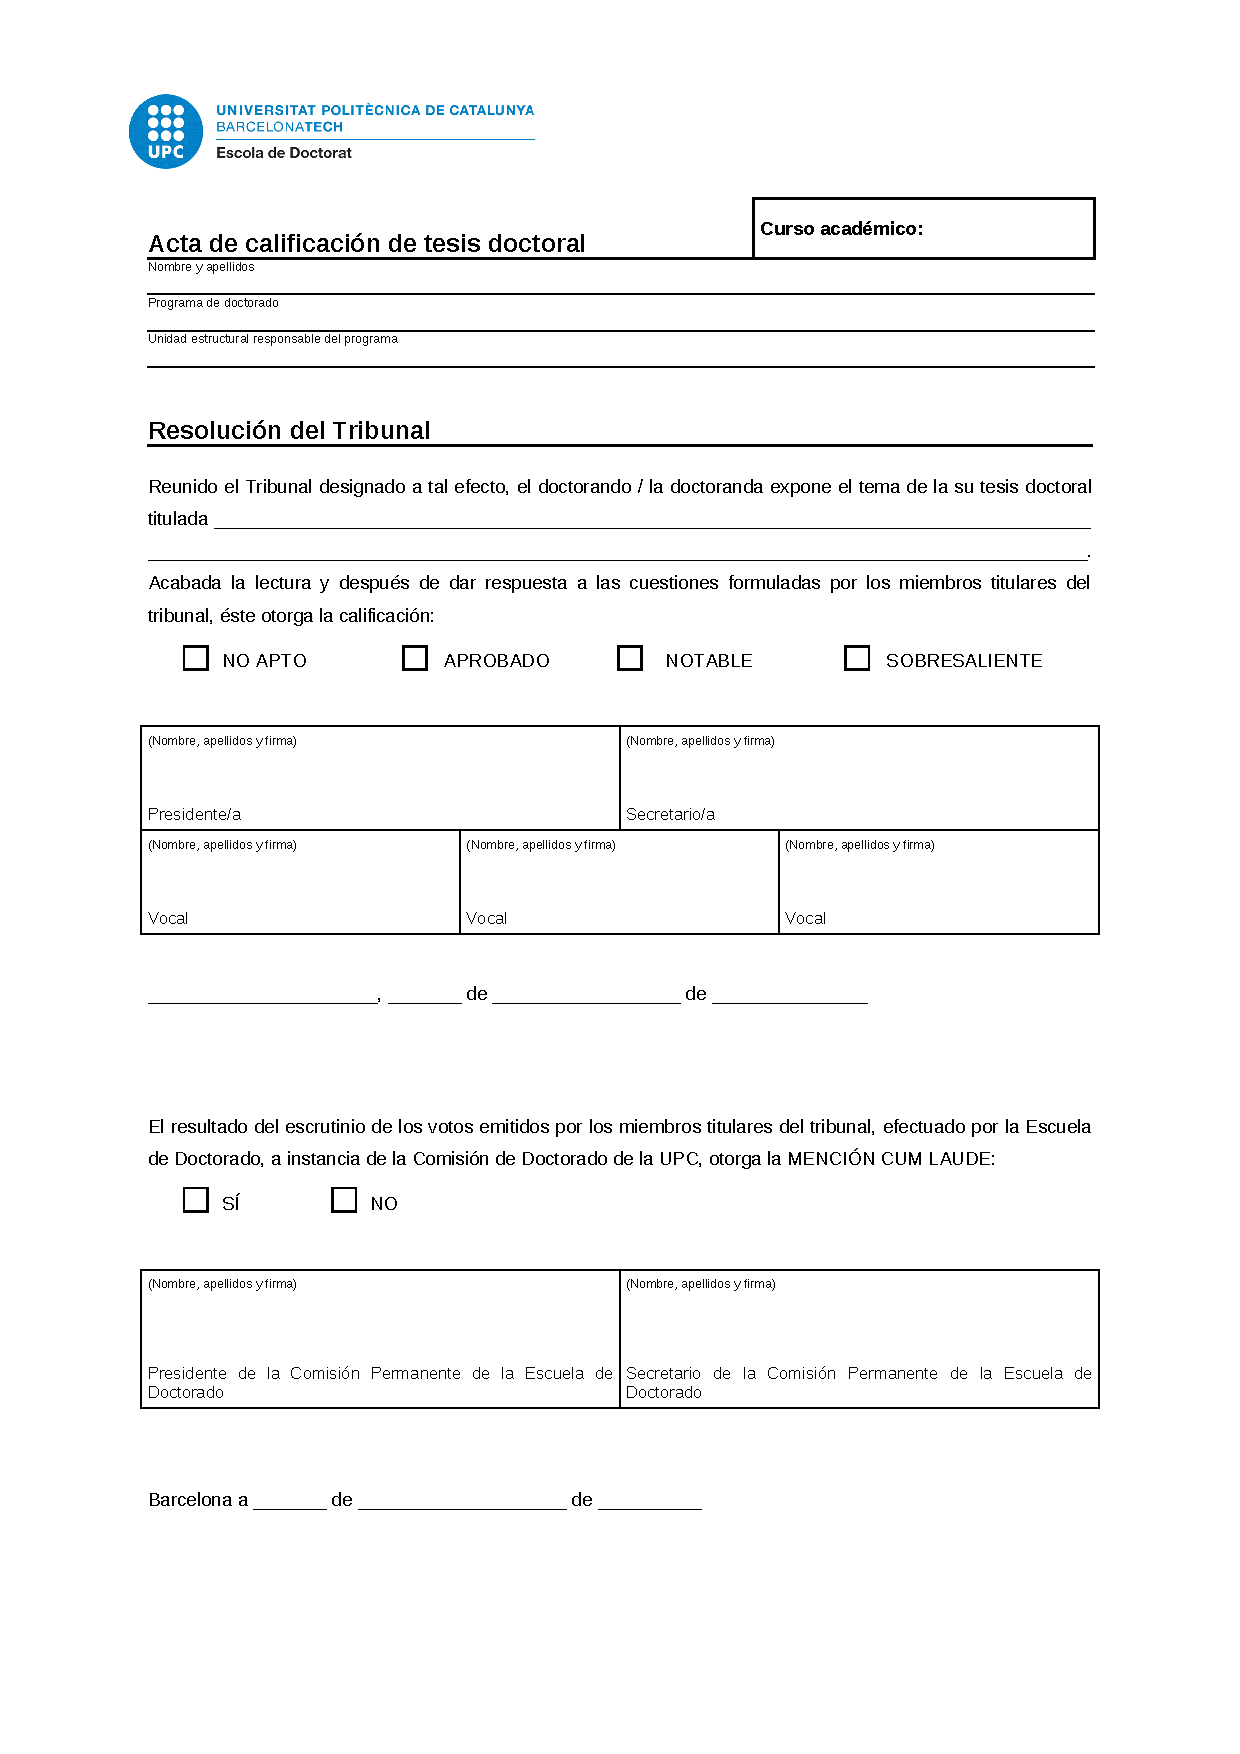
\includepdf[pages={1}]{acta.pdf}

\ifdefineAbstract
 \pagestyle{empty}
 \includeonly{preface/declaration, preface/abstract}
\fi

% ***************************** Chapter Mode ***********************************
% The chapter mode allows user to only print particular chapters with references
% Title, Contents, Frontmatter are disabled by default
% Useful option to review a particular chapter or to send it to supervisior.
% To use choose `chapter' option in the document class

\ifdefineChapter
 \includeonly{Chapter3/chapter3}
\fi

% ******************************** Front Matter ********************************
\begin{document}

\frontmatter

\maketitle

%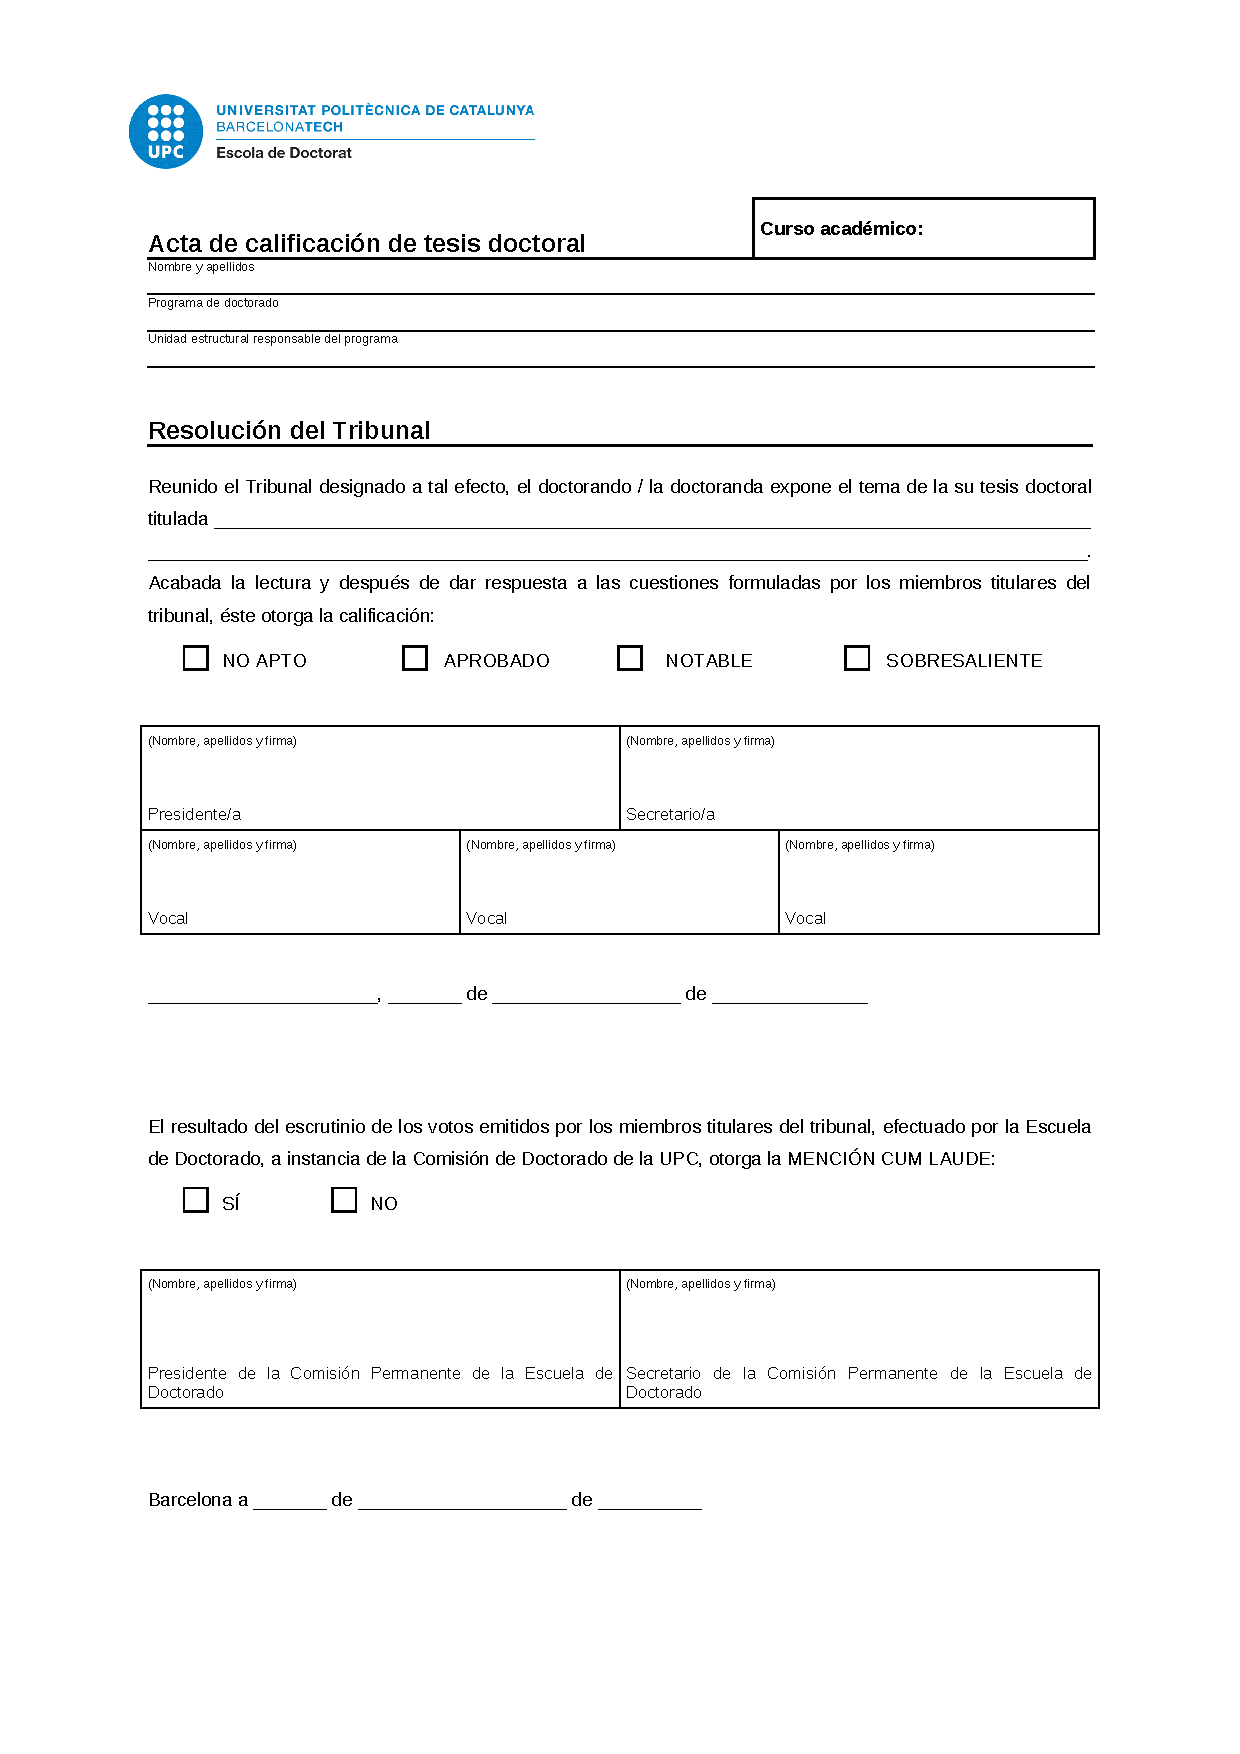
\includegraphics{acta.pdf}
%\clearpage
%\mbox{}
%\clearpage
\newpage\null\thispagestyle{empty}\newpage
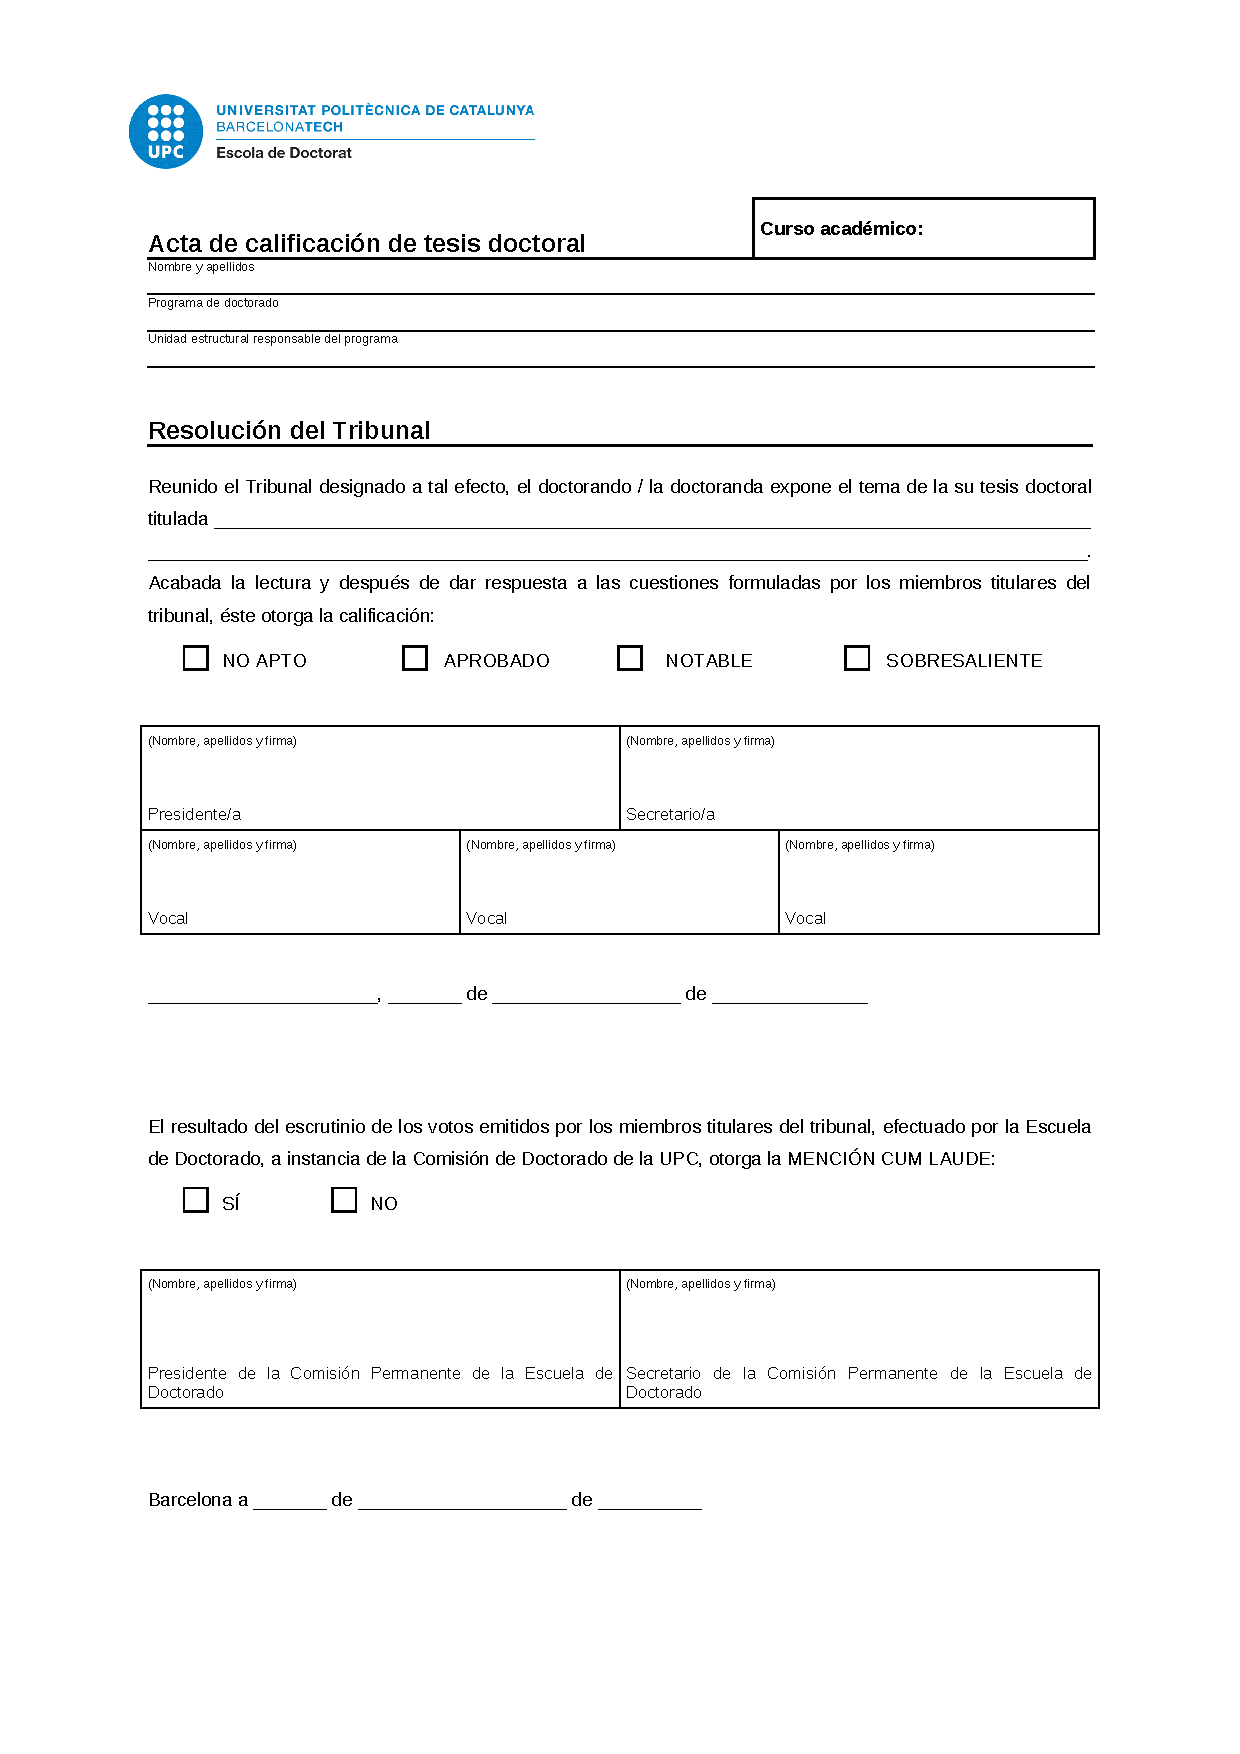
\includepdf[pages=-]{acta.pdf}
\clearpage

\begin{abstract}

\end{abstract}


\begin{dedication}
To my family and friends.

%\vspace*{\fill}
%To think that there at some point in time, someone had the audacity to look
%towards the night sky, where the rest of us remained buffled and silent in
%front of the majesty of the heavens... and blinked in front of the
%incoprehensive vastness of space, and kept at it till all the stars were known.
%\vspace*{\fill}

\end{dedication}

\newpage\null\thispagestyle{empty}\newpage


%\clearpage\mbox{}\clearpage
\vspace*{200pt}
\epigraph {I do not know what I may appear to the world, but to myself I seem to have been
only like a boy playing on the sea-shore, and diverting myself in now and then finding a
smoother pebble or a prettier shell than ordinary, whilst the great ocean of truth lay all
undiscovered before me.}{— Isaac Newton}

%\include{Declaration/declaration}

\begin{acknowledgements}
	I would like to extend my gratitude and appreciation to my advisors Dr. Marc
	Casas and Dr. Eduard Ayguad\'{e}, without their patience and guidance this
	thesis would not have been possible. I would also like to thank Dr.
	Cristiano Malossi and Dr. Panagiotis Hadjidoukas from IBM Z\"{u}rich Lab
	who, during the course of our collaboration, gave me valuable feedbacks and
	insights that lead to the success of my work. As well as for their
	hospitality during my month-long stay in Z\"{u}rich that warmed a lone
	traveler's heart.

	It has been a long five-year journey. One does not simply navigate through
	those times alone, not to mention the place I call home is ten thousand km
	away. I want to thank those who were or still are by my side giving me
	support, talking me through things when the getting is tough. My
	appreciation goes to my bestie Kallia, along with Rajiv, Danai, Tomasz and
	David with whom we shared invaluable moments and countless chuckles during
	the good part of my PhD. To Ariel, a close friend that we get along well enough
	to consider sharing an apartment with. To Ilia and Klaudia who we shared a close
	connection despite the little time we spent. Last but not least, a group of
	people of all ages and from all walks of life yet have enough synergy to
	form a close group that I came across over the final months of my PhD: Alex,
	Asaf, Ettore, John "El Cucho" Osorio, Louis "LeDur" Ledoux, Robin and
	Tamara. A group that offers laughters and stories that makes an otherwise
	stressful conclusion of a PhD a lot more entertaining.	

	%This thesis has been supported by the Spanish Government (Severo Ochoa grants
	%SEV2015-0493, SEV-2011-00067), by the Spanish Ministry of Science and
	%Innovation (contracts TIN2015-65316-P), by Generalitat de Catalunya
	%(contracts 2014-SGR-1051 and 2014-SGR-1272), by the RoMoL ERC Advanced
	%Grant (GA 321253) and the European HiPEAC Network of Excellence.  This
	%work was also partially performed under the auspices of the U.S.
	%Department of Energy by Lawrence Livermore National Laboratory under
	%Contract DE-AC52-07NA27344 (LLNL-CONF-689878).
\end{acknowledgements}

\thispagestyle{empty}

% *********************** Adding TOC and List of Figures ***********************

\glsaddall

\tableofcontents

\clearpage
%\printglossary
% \printnomenclature[space] space can be set as 2em between symbol and description
%\printnomenclature[3em]

%\printnomenclature

% ******************************** Main Matter *********************************
\mainmatter

\chapter{Introduction}
\label{chap:introduction}
Modern parallel systems make extensive use of their massive amount of CPU core 
counts or their peripheral accelerators (GPU, FPGA, ASIC etc.). In order to 
effectively parallelize the problem at hand, algorithm designers need to 
meticulously split the problem into smaller chunks that can be executed on the 
individual computational units. \textbf{\textcolor{red}{expansion needed}}

Not all problems are created equal. For some, denoted as \textit{embarrassingly parallel}, 
the task is relatively simple because they can be easily solved in a divide and 
conquer fashion. Each component is inherently independent in that it does not 
require the computational results from its counterparts. 
\textbf{\textcolor{red}{examples, refs}}

Others on the other hand, oftentimes have non-parallelizable sections that 
create interleaving parallel-sequential-parallel patterns during the execution where 
synchronization is required. It is also a commonplace that parallel sections 
possess dependencies in which case communication inevitably occur.
\textbf{\textcolor{red}{examples, refs}}

As peripherals, the various types of accelerators are connected through external 
buses like PCI, NVlink etc. Necessary data has to be transferred from the host 
CPUs to the accelerators before carrying out any meaningful computation. It is 
prominent among iterative-based numerical methods and with the rise of deep 
neural networks.

Synchronization and communication put the involved computational units on hold 
thus impede the execution progress. The scale of the parallel system is the 
primary impact factor of the efficiency of the communication for the following 
reasons.
\begin{itemize}
    \item The physical proximity of the communicating nodes determines the 
        quality of the communication. In a distributed system with nodes scattered 
        at different physical locations, the communication inbalance could create 
        serious bottlenecks.
    \item The need to send data back and forth is alleviated on a shared-memory 
        system where all the computational units have access to entire memory region. 
        Nevertheless, such systems are inherently limited by size. Another type 
        of underlying memory hierarchy is distributed-memory systems where each 
        node is in possess of a portion of the entire memory. The acquisition 
        of contents from other memory regions has to be resolved by passing 
        messages which could raise contention on the bus system.
\end{itemize}
 
\section{Thesis Objectives and Contributions}
This thesis strives to alleviate the communication by reducing either the 
occurrences of communication points or the quantity of data in the domain of 
iterative numerical methods and deep neural networks, while in the meantime 
retaining the quality of the results the algorithms produce. 

\subsection{Communication Reduction in Conjugate Gradient Method}
The conjugate gradient method solves a linear system in an iterative manner. 
Conventionally, synchronization is needed at the end of each iteration in a 
parallel implementation for some bookkeeping tasks such as checking the 
convergence and applying the residual replacement strategy. 
We propose the \emph{Iteration-Fusing Conjugate Gradient} which fuses some of the 
iterations by removing the inter-iteration synchronization points within those fused 
iterations and moving the bookkeeping tasks to the end of the last iteration from the fusion. 
Also we use a task-based parallel programming model to split numerical kernels 
into subkernels to relax data-dependencies. By carrying out these two optimizations, 
our approach allows computations belonging to different iterations to overlap if 
there are no specific data or control dependencies between them.
The main contributions of this approach are:
\begin{itemize}
       \item The Iteration-Fusing Conjugate Gradient (IFCG) approach, which aims 
           at aggressively overlapping different iterations. IFCG is implemented 
           by means of two algorithms: IFCG1 and IFCG2.
       \item A task-based implementation of the IFCG1 and IFCG2 algorithms that 
           automatically overlaps computations from different iterations without 
           the need for explicit programmer specification on what computations should be overlapped.
       \item A comprehensive evaluation comparing IFCG1 and IFCG2 with the most 
           relevant state-of-the-art formulations of the CG algorithm. 
           IFCG1 and IFCG2 provide parallel performance improvements up to 42.9\% 
           and 41.5\% respectively and average improvements of 11.8\% and 7.1\% with 
           respect to the state-of-the-art techniques and show similar numerical stability.
        \item A demonstration that under realistic system noise regimes IFCG 
            algorithms behave much better than previous approaches. IFCG algorithms 
            achieve an average 18.0\% improvement over the best state-of-the-art 
            techniques under realistic system noise regimes.
\end{itemize}

\subsection{Communication Reduction in Training Deep Neural Network Models}
We describe and evaluate a method to accelerate the training of DNNs by reducing the cost 
of data transfers across heterogeneous high-end architectures integrating multiple GPUs. By relying on DNNs 
tolerance to data representation formats smaller than the commonly used 32-bit Floating 
Point (FP) standard~\cite{gupta15, flexpoint17}, we describe how to dynamically adapt 
the size of data sent to GPU devices without hampering the quality of the training process. 
Our solution is designed to efficiently use the incoming bandwidth of the GPU accelerators.
It relies on an adaptive scheme that dynamically adapts the data representation format required 
by each DNN layer and compresses network parameters before sending them over the parallel system.
This scheme enables DNNs training to progress in a similar rate as if the 32-bit FP format was used.
This work makes the following contributions:
\begin{itemize}
    \item It proposes the {\it Adaptive Weight Precision (AWP)} algorithm, which 
        dynamically adapts the numerical representation of DNN weights during training. 
        AWP relies on DNNs' tolerance for reduced data representation formats.  
        It defines the appropriated data representation format per each network layer during  
        training without hurting network accuracy.

    \item It proposes a new {\it Approximate Data Transfer (ADT)} procedure to compress 
        DNN's weights according to the decisions made by the AWP algorithm. 
        ADT relies on both thread- and SIMD-level parallelism  
        and is compatible with architectures like IBM's POWER 
        or x86. ADT is able to compress large 
        sets of weights with minimal overhead, which enables the large performance benefits of our approach.

    \item It evaluates ADT and AWP on 
        two high-end systems: The first is composed of two x86 Haswell multicore 
        devices plus four Tesla GK210 GPU accelerators and the second system integrates two POWER9 chips and four NVIDIA Volta V100 GPUs. 
        Our evaluation considers the Alexnet~\cite{alexnet}, the VGG~\cite{vgg} and the Resnet~\cite{resnet} network models applied to 
        the ImageNet ILSVRC-2012 dataset~\cite{imagenet}.
        Our experiments report average performance benefits of 6.18\% and 11.91\% on the x86 and the POWER systems, respectively.
        Our solution does not reduce the quality of the training process since networks final accuracy is the same as if they had been trained with the 32-bit Floating Point format.
\end{itemize}

\subsection{Communication Reduction in Deep Learning Model Parallelism}


\section{Thesis Structure}

\chapter{Background}
\label{chap:background}
This section provides a description on the state-of-the-art and the current 
challenges presented in the field of parallel computing and deep learning in 
order to grasp the works carried out from this thesis.
Section~\ref{sec:mps} prepares the reader with the acquaintances of the various 
forms of modern parallel systems. Section~\ref{sec:ppm} provides background on 
the parallel programming models on modern parallel systems. Subsequently, 
section~\ref{sec:solvers} and~\ref{sec:dnn} present an introduction to the two 
application domains this work deals with, namely, parallel numerical algorithms 
and DNNs.

\section{Modern Parallel Systems}
\label{sec:mps}
Exascale supercomputers are expected to come into operation near 2020. In order 
to reach that, major improvements need to be achieved including the energy and 
power, memory and storage, concurrency and locality and resiliency~\cite{doe}.  
Nevertheless, the mainstream trend stays with the massive parallelism with 
accelerators approach. This section provides a background on both types of 
systems and an introduction to some major parallel programming models.

With the roll-out of 7 and 5 nm node, the VLSI (very large scale integration) 
manufacturing technology is rapidly approaching its end due to its physical 
limitation. Furthermore, the power and energy consumption, as a consequence the 
heat dissipation, on a modern VLSI chip has become a major limiting factor in 
processor design. All the above impede the efforts to push a single-core 
processor to go faster. In response, industry turns its attention into designing 
multi-core multiprocessor systems which exploit parallelism at the application 
level. Figure~\ref{fig:multicore} illustrates a typical multi-core 
multiprocessor system~\cite{ibm_multicore}. Each of the processors (processor 0 
and 1) packs two separate cores with their own L1 and L2 caches. The two 
processors are connected via a system bus which also connects to the RAM. All 
the cores thus are able to access to the entire memory region. Nonetheless, 
since all the access to the memory and communication among processors are 
conducted on the system bus, the system is limited in its scale in that the 
inevitable contention on the bus system while the number of processors grows 
eventually renders a large-scale system unresponsive.
\begin{figure}[H]
    \centerline{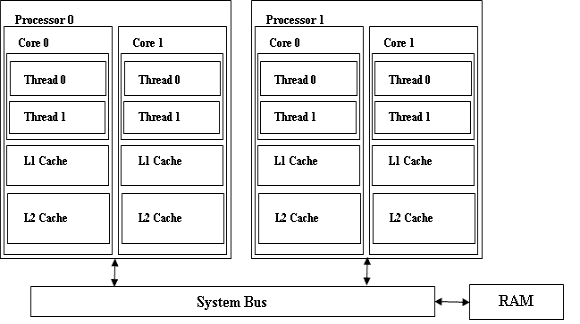
\includegraphics[scale=0.50]{background/figs/multicore_mp_system.png}}
    \caption{A typical chip multithreaded, multi-core, multiprocessor system}
    \label{fig:multicore}
\end{figure}

With the ever-growing demand of computation power, a large amount of such 
processors are grouped close together into a computer cluster with high speed 
interconnection system to further scale the system. All the cores belonging to 
the same node in the cluster shares the resources (memory system, last-level 
cache etc.) whereas cross-node resources are private to their respective nodes.  
This essentially segregates the memory system into various regions not directly 
accessible to all the cores. This type of memory system is known as 
distributed-memory system. Accessing remote contents is possible by sending them 
as message to the requesting node which implies that accessing to different 
memory regions incurs distinct latency.  This offloads the task of ensuring the 
performance of the program to the programmer because careless handling of the 
physical location and topology of the nodes can easily saturate the 
interconnection system and cause different processors to have imbalanced 
accessing time to the same data.

Since the dawn of the artificial intelligence, GPU, due to its immense data 
parallelism capability, has accelerated its transformation from a peripheral 
device used in niche domains to a general-purpose mass adoption. Along with the 
re-configurability of FPGAs and domain-specific ASICs, heterogeneous systems 
contribute to a significant portion of computation power on some modern parallel 
systems. As external devices, to be able to exploit their parallelism, data has 
to be transferred from the CPU to the device and vice versa in the face of any 
synchronization or communication. 

\section{Parallel Programming Models}
\label{sec:ppm}
Parallel programming models can roughly be categorized into two class: one for 
shared-memory systems and the other for distributed-memory systems. The 
classification is due to the distinct ways these models deal with the underlying 
memory system.

\subsection{Shared-Memory Programming Model}
OpenMP~\cite{openmp, OpenMP4.0} is a standard programming model on a 
shared-memory system. It is an application programming interface (API) that 
supports shared memory multiprocessing programming in C, C++, and FORTRAN.

OpenMP (prior to version 3.0) uses a fork-join model for its parallel executions 
as seen in Figure~\ref{fig:fork-join}.
All OpenMP programs begin as a single process: the master thread. The master 
thread executes sequentially until the first parallel region construct is 
encountered. The master thread then creates a team of parallel threads.
The statements in the program that are enclosed by the parallel region construct 
are then executed in parallel among the various team threads. When the team 
threads complete the statements in the parallel region construct, they 
synchronize and terminate, leaving only the master thread~\cite{llnl_openmp}.
\begin{figure}[H]
    \centerline{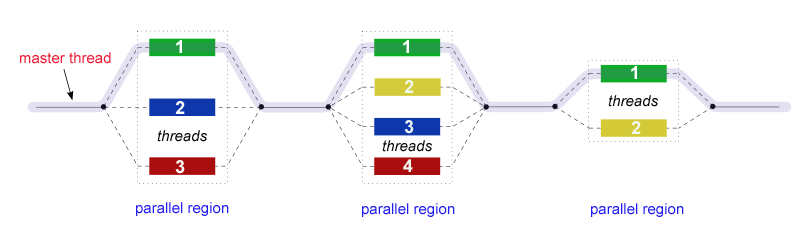
\includegraphics[scale=0.50]{background/figs/fork_join.png}}
    \caption{OpenMP uses a fork-join model}
    \label{fig:fork-join}
\end{figure}

\subsection{Task-based Parallel Programming Model}
A fork-join model creates parallel regions each of which is dedicated to solving 
a specific problem whereas the program logic is executed in sequential on the 
master thread. It introduces inefficiencies because the parallel regions can be 
far between and the sequential execution in-between keeps all the other threads 
idle. 

Task-based parallel programming model sets off to tackle this problem. In a 
task-based approach the problem is ideally re-factorized and decomposed into 
smaller functions called tasks that have clear set of inputs and outputs from 
which data dependencies can be derived unambiguously. Therefore, tasks can be 
launched and executed in parallel as long as they don't have data dependencies 
among each other and hardware resources are available. A dedicated runtime 
system is in charge of building the dependency graph and orchestrating the task 
scheduling. Figure~\ref{fig:task-dependency} illustrates a typical task 
dependency graph which is a DAG (directed acyclic graph) that the runtime system 
uses to check the pending dependencies. There are many task-based parallel 
programming models, the most prominent of which includes the OpenMP (version 3.0 
onwards)~\cite{OpenMP4.0}, Clik++~\cite{clik}, TBB~\cite{tbb} and 
OmpSs~\cite{ompss}.

\begin{figure}[H]
    \centerline{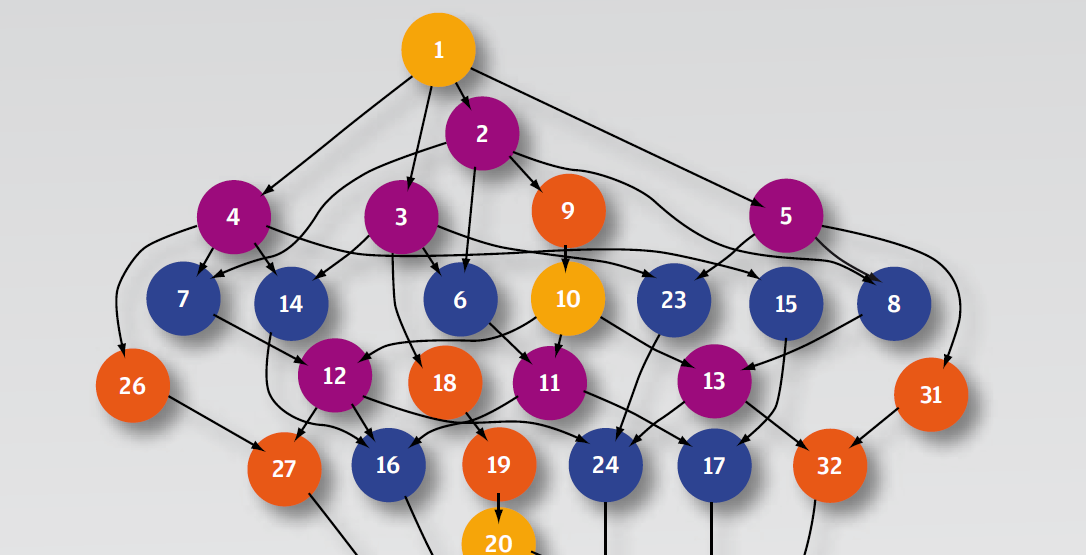
\includegraphics[scale=0.50]{background/figs/starss.png}}
    \caption{A typical task dependency graph}
    \label{fig:task-dependency}
\end{figure}

\subsection{Distributed-Memory Programming Model}
MPI (Message Passing Interface) is the main parallel programming paradigm for 
distributed memory environments. It is a library specification for 
message-passing, proposed as a standard by a broadly based committee of vendors, 
implementors, and users. It primarily addresses the message-passing parallel 
programming model: data is moved from the address space of one process to that 
of another process through cooperative operations on each 
process~\cite{llnl_mpi}.

The MPI interface is meant to provide essential virtual topology, 
synchronization, and communication functionality between a set of processes 
(that have been mapped to nodes/servers/computer instances) in a 
language-independent way, with language-specific syntax (bindings), plus a few 
language-specific features. MPI programs always work with processes, but 
programmers commonly refer to the processes as processors. 

MPI library functions include, but are not limited to, point-to-point 
rendezvous-type send/receive operations, choosing between a Cartesian or 
graph-like logical process topology, exchanging data between process pairs 
(send/receive operations), combining partial results of computations (gather and 
reduce operations), synchronizing nodes (barrier operation) as well as obtaining 
network-related information such as the number of processes in the computing 
session, current processor identity that a process is mapped to, neighboring 
processes accessible in a logical topology, and so on. Point-to-point operations 
come in synchronous, asynchronous, buffered, and ready forms, to allow both 
relatively stronger and weaker semantics for the synchronization aspects of a 
rendezvous-send~\cite{wiki_mpi}.

\section{Numerical Methods For Systems of Linear Equations}
\label{sec:solvers}
Systems of equations are used to represent physical problems that involve the 
interaction of various properties. The variables in the system represent the 
properties being studied, and the equations describe the interaction between the 
variables. The system is easiest to study when the equations are all linear.  
Often the number of equations is the same as the number of variables, for only 
in this case is it likely that a unique solution will exist. Although not all 
physical problems can be reasonably represented using a linear system with the 
same number of equations as unknowns, the solutions to many problems either have 
this form or can be approximated by such a system. In fact, this is quite often 
the only approach that can give quantitative information about a physical 
problem. The problem is to find the vectors of unknown $x$ in $Ax = b$
$$
A=
\begin{pmatrix}
    a_{11}&a_{12}&...&a_{1n}\\
    a_{21}&a_{22}&...&a_{2n}\\
    ...&...&...&...\\
    a_{m1}&a_{m2}&...&a_{mn}\\
\end{pmatrix}
$$
where $x \in \Re^n$, $b \in \Re^m$ and $A \in \Re^m$ x $\Re^n$.

Two classes of numerical methods are available for solving the system:
\begin{itemize}
    \item Direct Methods that provide the exact solution $x$ by a finite 
        sequence of operations.
    \item Iterative Methods that start with a first approximation $x^{(0)}$ and 
        compute in an iterative manner a sequence of approximations $x^{(i)}$, 
        in the hope to obtain increasingly better results, without ever reaching 
        $x$.
\end{itemize}

\subsection{Direct Methods}
A common way to obtain the exact numerical results of systems of linear 
equations is using matrix factorization.

LU factorization of a matrix is the factorization of a given square matrix into 
two triangular matrices, one upper triangular matrix and one lower triangular 
matrix, such that the product of these two matrices gives the original matrix.  
The LU factorization method comes handy whenever it is possible to model the 
problem to be solved into matrix form. Conversion to the matrix form and solving 
with triangular matrices makes it easy to do calculations in the process of 
finding the solution~\cite{mc, nla}.

For $$ A=
\begin{pmatrix}
    a_{11}&a_{12}&a_{13}\\
    a_{21}&a_{22}&a_{23}\\
    a_{31}&a_{32}&a_{33}\\
\end{pmatrix} $$ we have
$$ L=
\begin{pmatrix}
    1      &  0       &  0  \\
    l_{21} &  1       &  0  \\
    l_{31} &  l_{32}  &  1  \\
\end{pmatrix} $$ and $$ U=
\begin{pmatrix}
    u_{11} &  u_{12}  &  u_{13}  \\
    0 &  u_{22}  &  u_{23}  \\
    0 &  0  &  u_{33}  \\
\end{pmatrix} $$ such that $A = LU$. The system of equations $Ax = b$ can thus 
be solved by the following steps:
\begin{enumerate}
    \item Factorize the matrix $A$ so that $LUx = b$
    \item Solve the equation $Ly = b$ for $y$ by forward substitution
    \item Solve the equation $Ux = y$ for $x$ by backward substitution
\end{enumerate}

Cholesky factorization is a faster method if the matrix $A$ is symmetric 
positive-definite. In which case $A$ can be factorized into $A = LL^T$ where 
where $L$ is a lower triangular matrix with real and positive diagonal entries, 
and $L^T$ denotes the transpose of L~\cite{nla}.

\subsection{Iterative Methods}
In the absence of rounding errors, direct methods would yield an exact solution 
yet iterative methods are indispensable when facing linear problems involving a 
large number of variables (in the order of millions or more), where direct 
methods would be prohibitively expensive even with the best available computing 
power~\cite{nla}. 

Krylov methods are among the most successful iterative methods and see a wide 
application in numerical linear algebra. Krylov subspace methods solves a linear 
system $Ax = b$ by forming a basis of the sequence of successive matrix powers 
times the initial residual, \{$b, Ab, A^2b, \ldots, A^mb$\}. The approximations 
to the solution are then formed by minimizing the residual over the subspace 
formed. The prototypical method in this class is the conjugate gradient method 
(CG)~\cite{cg} which assumes that the system matrix $A$ is symmetric 
positive-definite. For symmetric (and possibly indefinite) $A$ one works with 
the minimal residual method (MINRES)~\cite{minres}. In the case of not even 
symmetric matrices methods, such as the generalized minimal residual method 
(GMRES)~\cite{gmres} and the biconjugate gradient method (BiCG)~\cite{bicg}, 
have been derived.

\section{Deep Supervised Learning and Its Parallelization}
\label{sec:dnn}
Deep learning uses multi-layer neural networks to carry out wide range of tasks 
such as image recognition~\cite{alexnet},  video 
classification~\cite{video_class}, various NLP (natural language processing) 
tasks~\cite{nlp0, nlp1, nlp2, nlp3} and art generation~\cite{gan, can} just to 
name a few. A neural network consists of layers of neurons which are themselves 
a mathematical model of a linear classifier. Figure~\ref{fig:perceptron} depicts 
the inner workings of a neuron. The neuron takes a vector of inputs $x$, first 
calculate its weighted sum $y = \sum_{i=1}^{n} x_i w_i$ and apply a non-linear 
step function $o = \delta(y)$. An MLP (multi-layer perceptron) is thus comprised 
of multiple layers each of which is constituted of multitudes of neurons with 
their respective set of weights per input.
\begin{figure}[H]
    \centerline{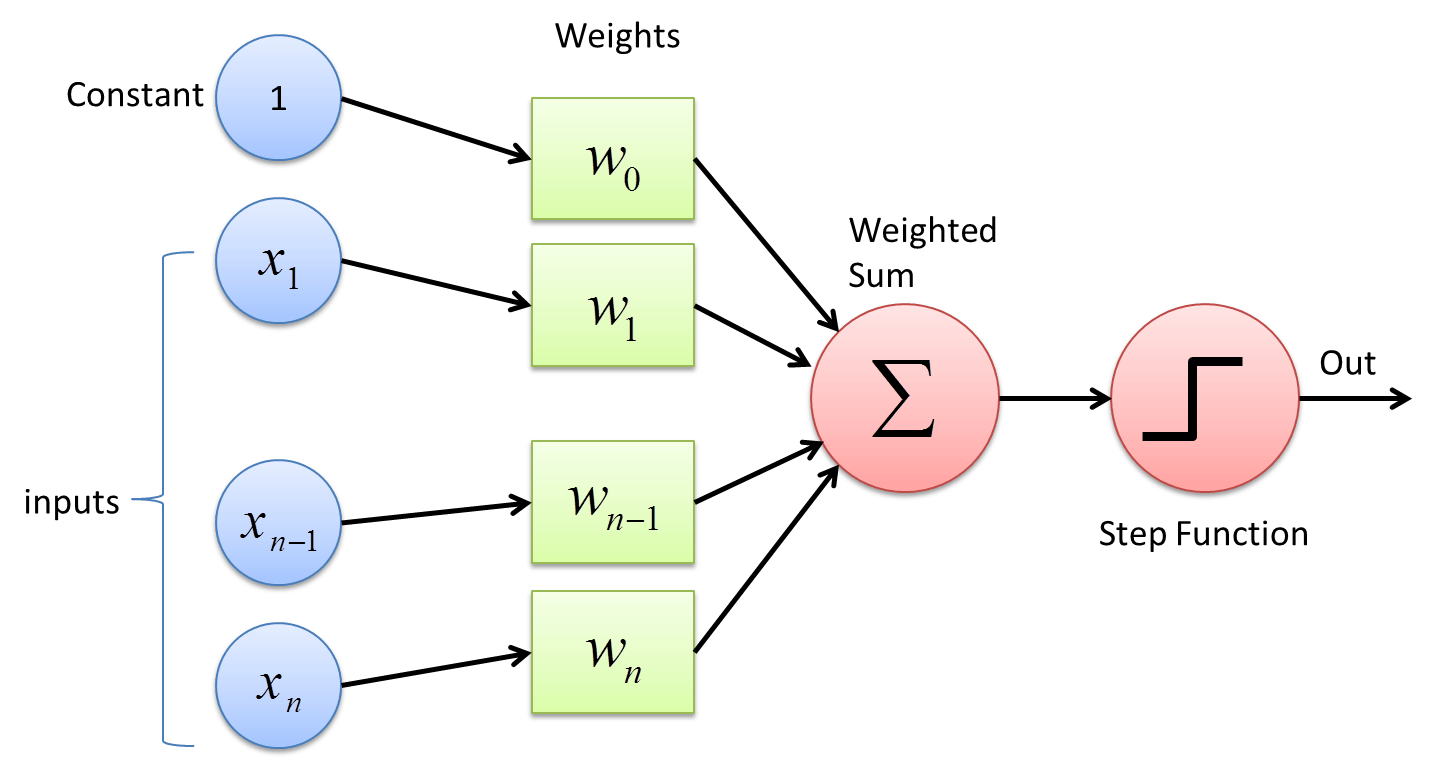
\includegraphics[scale=0.25]{background/figs/perceptron.png}}
    \caption{The workings of a neuron}
    \label{fig:perceptron}
\end{figure}

This thesis has its focus on one particular branch of the deep learning, namely, 
deep supervised learning. It utilizes a MLP (multi-layer perceptron) or CNN 
(convolutional neural network) to learn a function that maps an input to an 
output based on example input-output pairs. It infers a function from labeled 
training data consisting of a set of training examples. The dataset in 
supervised learning are a pair of input and a ground truth (the desired output).
The neural network learns by adjusting all the weights from each neuron 
according to its gradient $w' = w - \mu \Delta w$ to the lost yielded by a loss 
function that measures the difference of the output of the neural network and 
the ground truth. A typical loss function is MSE (mean square error), cross 
entropy etc.

\subsection{Parallelism in Deep Learning}
Effectively training a neural network demands an immense amount of data. This 
inevitably raise the need for parallelization. Currently, there are two 
paradigms:
\begin{itemize}
    \item Data parallelism aims to run the training on data batches 
        simultaneously.
    \item Model parallelism aims to split the neural network itself to available 
        computation units.
\end{itemize}

\subsubsection{Data Parallelism}
The most common way in the data parallelism paradigm is the use of a parameter 
server~\cite{pserver}. The dataset is split into data shards that are 
consequently fed to each and every computation units respectively. The 
parameters (weights $w$, biases $b$ etc.) are stored separately in dedicated 
units called parameter servers. At the beginning of each batch of the training, 
all the computation units involved in the training request a up-to-date copy of 
the parameters from the servers. They carry on with the training and at the end 
of the batch send their respective gradient $\Delta w$, $\Delta b$ back to the 
servers. The servers then are responsible for updating the parameters with 
regard to the gradients. Figure~\ref{fig:pserver} illustrates a schematic of two 
parameter servers and three trainers.
\begin{figure}[H]
    \centerline{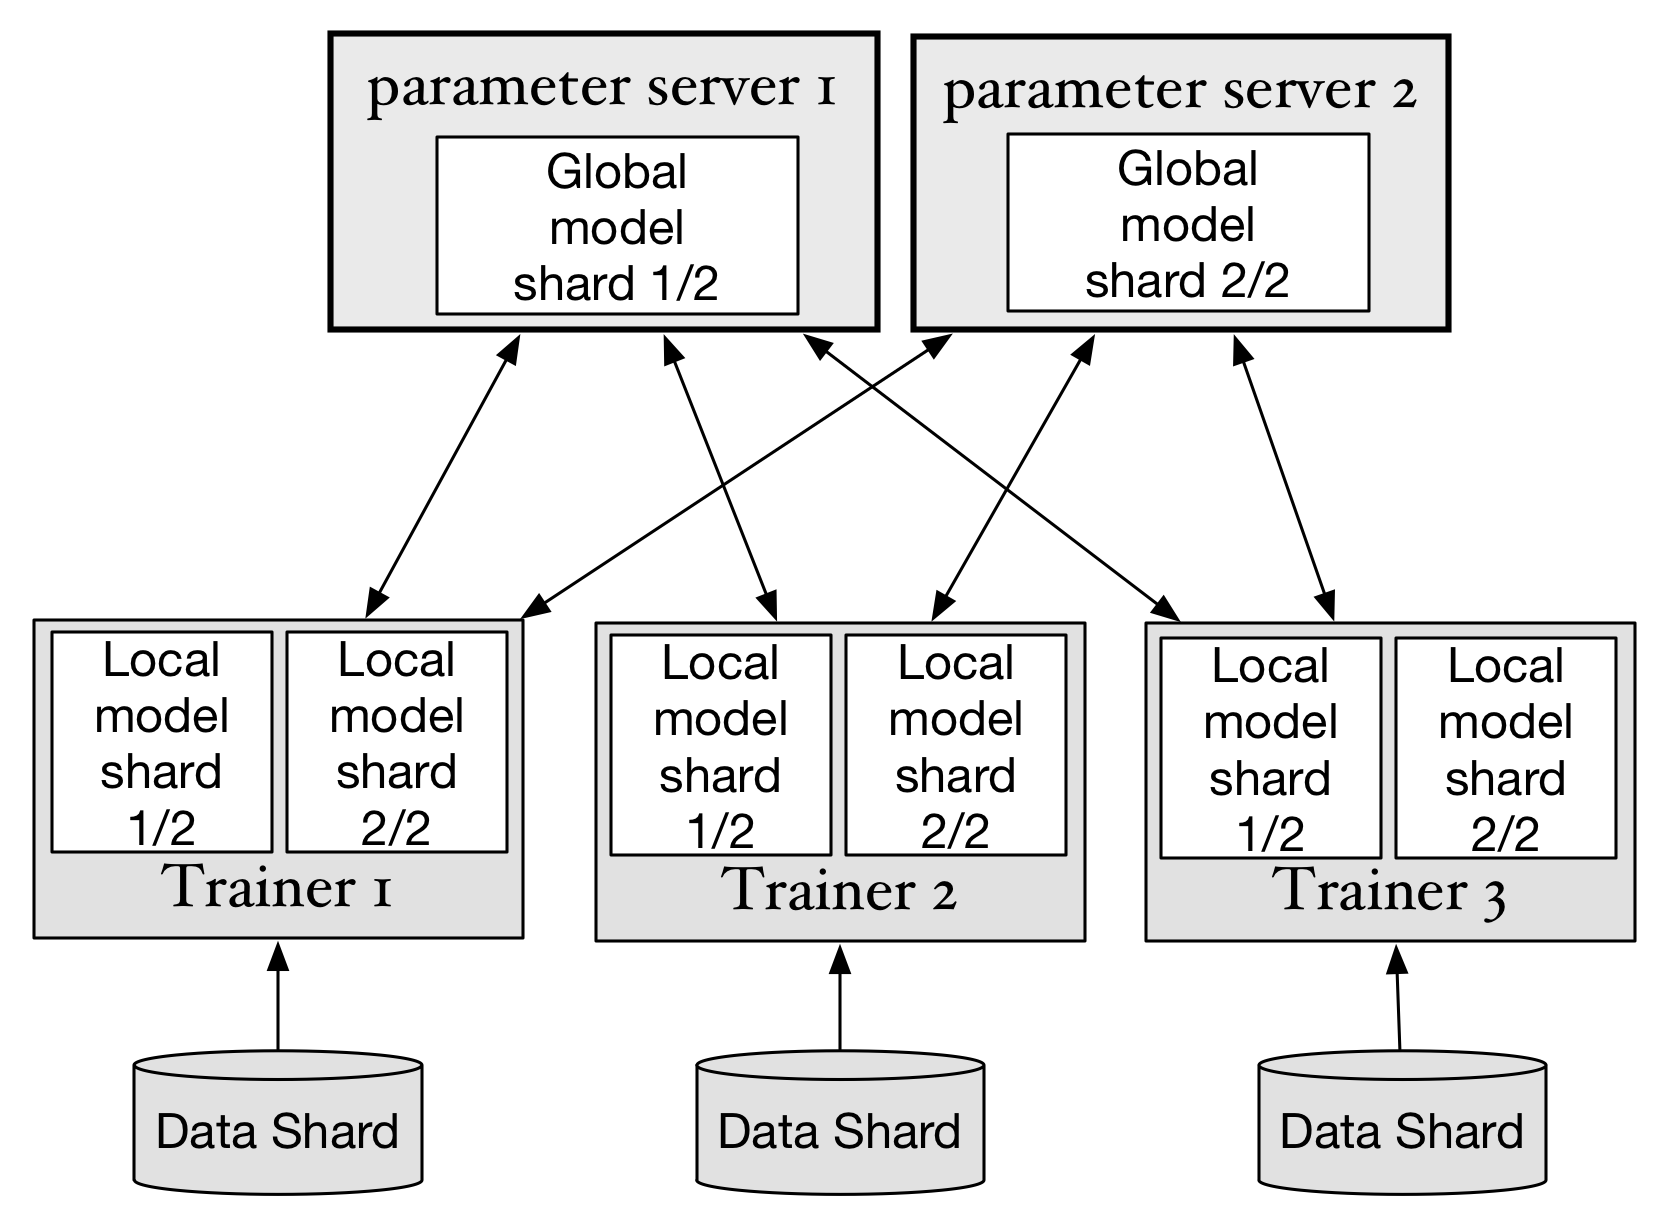
\includegraphics[scale=0.40]{background/figs/data_parallelism.png}}
    \caption{Two parameter server and three trainers}
    \label{fig:pserver}
\end{figure}

\subsubsection{Model Parallelism}
Model parallelism is also called network parallelism. It can be seen as a 
orthogonal to data parallelism. This strategy divides and distributes part of 
the network to different machines. Figure~\ref{fig:model} shows the difference 
between data and model parallelism. Model parallelism is suitable for models 
that are too large to fit into one machine but this comes at a cost of incurring 
additional communication during one batch of training~\cite{model0}.
\begin{figure}[H]
    \centerline{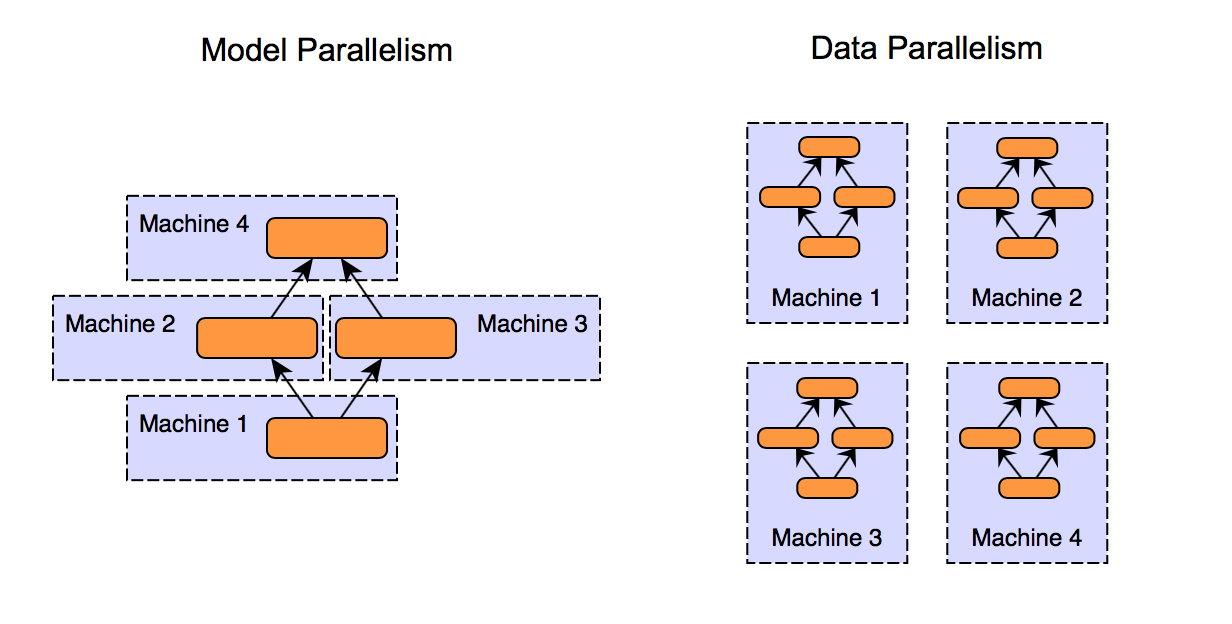
\includegraphics[scale=0.60]{background/figs/model_parallelism.png}}
    \caption{The difference between data and model parallelism}
    \label{fig:model}
\end{figure}

Nevertheless, the DNN architecture creates layer interdependencies, which, in 
turn, generate communication that determines the overall performance. Fully
connected layers, for instance, incur all-to-all communication (as opposed to 
allreduce in data parallelism), as neurons connect to all the neurons of the 
next layer~\cite{model1}.


\chapter{Experimental Setup}
\label{chap:methodology}

In this Chapter we describe the hardware and software platforms used for the experimental
evaluation of this work.  In this work we assume that we work with parallel workloads that
are implemented with a programming model that allows dynamically controlling its
concurrency level.  Applications should also be able to be decomposed into concurrent
tasks.  The underlying hardware platform should offer the ability to impose user defined
power caps, at least per each socket (such as Intel CPU models that are equally or older
than the Sandy Bridge family of processors).  Moreover, older CPU models do not
demonstrate notable manufacturing variability.
We also assume the presence of a workload manager to manage running applications on an 
HPC cluster.   

\section{Hardware Platforms} 
\label{sec:platforms}
For our experimental evaluation we use two distinct HPC
clusters, the MareNostrum III supercomputer at Barcelona Supercomputing Center and the
Catalyst and Quartz clusters at Lawrence Livermore National Lab.  Marenostrum III is one
of Europe's largest supercomputers and represents the state-of-the-art in production
environments in HPC.  Our initial evaluation of the PARSECSs is conducted on MareNostrum
III, however, since it's a large production machine, access to specific MSR registers,
required for monitoring and capping power on Intel chips, is restricted.  For this reason
we also use the Catalyst and Quartz cluster, where MSRs are accessible by the user through
special kernel modules. 

\begin{itemize}
	\item \emph{MareNostrum III}: It consists of 3,056 compute nodes in total. Each node is
IBM System X server iDataPlex dx360 M4, composed of two 8-core Intel Sandy Bridge
processors E5-2.60Hz, 20MB of shared last-level cache. There are eight 4GB DDR3 DIMM's
running at 1.6GHz (a total of 32GB per node and 2GB per core). 

	\item \emph{Catalyst}: The Catalyst cluster~\cite{llnlconfluence} consists of 324 NUMA
nodes, each with two 12-core Intel Xeon E5-2695v2 sockets and equipped with 128GB of main
memory.  It can reach a peak performance of 149.3 PFLOPS.  Access to MSR counters is
granted to normal users through a kernel module.  We use 128 of these nodes (256 sockets)
in our experiments, which totals to 3,072 cores.

	\item \emph{Quartz}: The Quartz cluster~\cite{llnlconfluence} consists of 2,634 NUMA
nodes, each with two 16-core Intel Xeon E5-2695v4 sockets and equipped with 128GB of main
memory.  It can reach a peak performance of 3,251.4 PFLOPS.  For our experiments we use We
use 128 of these nodes (256 sockets) in our experiments (4,096 cores in total).  As with
the case of Catalyst, access to the RAPL interface is granted through a kernel module.
This is a larger production machine we use to gather application execution traces and later
use in our workload manager simulator.

\end{itemize}

\section{Software Stack}

\subsection{Runtime System}
We use the OpenMP 4.0 standard to implement the PARSECSs benchmark suite.  We make use of
the Nanos++ OpenMP runtime system (version 0.8a).  Because of it's modular design it is
ideal to expand it's functionality and offers all OpenMP 4.0 features along with some
experimental ones.  Note that we only use the standard OpenMP 4.0 features in our
implementation.  We also use Nano++ for developing our power-aware runtime approach.
Nanos++ is coupled with the Mercurium source-to-source compiler (version 1.99), and gcc
4.7 as the back-end compiler.  
%To analyze the behavior of the \PARSEC{} benchmark suite (version 3.0), we use the Extrae
%instrumentation package~\cite{Labarta2006} (version 2.5) and the Paraver trace
%viewer~\cite{Labarta2006} (version 4.5). 
%We run all benchmarks using their respective native inputs as described in Table~\ref{tab:parsec}. 

\subsection{Analysis tools and Power Capping Framework}
We use a number of tools to perform various types of analyses on our benchmarks.  We use
the Extrae instrumentation package~\cite{Labarta2006} (version 2.5) and the Paraver trace
viewer~\cite{Labarta2006} (version 4.5) to analyze and compare the PARSEC and PARSECSs
benchmark suites.
 

\textit{Performance and Power Monitoring} 
Our methodology requires to monitor performance counters plus power consumption rates.  We
use \textit{perf} version 3.10 and \textit{mpstat} version 10.5.1 for monitoring
architectural and core component activity.  For measuring power and enforcing power limits
we use Intel's RAPL registers, which expand typical hardware counters, offering precise
readings on power consumption and temperature, as well as offering the functionality to
constrain core power consumption to a certain limit.  On Sandy and Ivy Bridge CPUs, these
special registers are accessible per socket, but on newer architectures like Haskwell,
they offer the same features per core.  We implement a daemon built on top of
\textit{libmsr}~\cite{libmsr}, which is a user friendly framework for accessing RAPL
registers safely from user space, through a special kernel module.  Our study focuses on
the variability on processors.  In our experiments we measured variance in DRAM power
consumption of less than 1\% (measured using the RAPL interface), among different
sockets when running the same benchmark.  For this reason, we only report the power 
consumption of processors.  We use the same framework for power capping sockets on
Catalyst and Quartz.  These power caps are enforced at hardware level by reducing the 
effective frequency of all cores, to match the requested power budget.
The user can specify a time window and a maximum average power for that window.
The processor guarantees that it will not exceed this average.
Intuitively, longer windows may allow better performance
for applications that utilize the CPU in bursts; if the burst
exceeds the window size, the processor will have to be
throttled.

The sample rate is 100ms for power monitoring and 1s for performance counters.  Although
we are able to monitor an applications real power consumption on a finer grain, our
predictions are limited to 1s granularity, since they depend on the performance counter
data collected at the coarser granularity.

\section{Workload Manager Simulator}
\label{sec:simulator}
For testing our scheduling policies, we implement a discrete event simulator, and
implement our scheduling policies on top of it.  Although there already exist workload
manager simulators for SLURM \cite{slurm_sim} and Flux \cite{flux_sim}, they do not model
power.  Moreover, these simulators also require tracing the applications.  We found it to
be more practical to implement our own to better control what traces need to be generated
and how power is to be handled and modeled. 

The simulator  requires all jobs to be first executed on the physical hardware
to gather performance and power profiles,  which are then used to simulate
their execution under different scheduling schemes. The performance and power
profiles are referred to as traces in this document.  They track performance
and power information over time, throughout a job's execution.  These traces
are different to job queues' traces, which contain information on the time a
job is issued, scheduled and completed, as well as which resources were
allocated for its execution.  Idle power is modeled as the average power consumed by each
socket, as measured on the actual hardware.  Using a simulator allows us to
rapidly test and evaluate new policies without any accuracy loss since the
simulations are led by power traces obtained from real parallel executions.
Our design allows the user to implement scheduling policies using python
scripts.  In our setup we implement SLURM's \cite{slurm_02} default job
scheduling policy, since it's the de-facto resource management tool on
production clusters.  The additional policies suggested by this work expand the
functionality of SLURM's default scheduler with power- and
variability-awareness.

\subsubsection{Validation of Workload Manager Simulator}
To validate the simulator we run a small scale experiment using 8 nodes (16
sockets) on Quartz.  The workload we use consists of a mix of a 100 instances
of the PARSECSs benchmarks.  Each instance is a single socket job and is
randomly chosen out of the total 10 PARSECSs benchmarks.  We run a bash script
that periodically issues 10 instances (every 60s) until all the job instances
are issued.  Then, it waits for all jobs to finish execution.  We generate a
trace with the timestamp of when every job was issued and on which node it was
run on.  We also keep track of the total time it takes for all the jobs to
complete along with the total energy the sockets consumed (including idle time).        

We then use the simulator to repeat the experiment and reproduce the results measured on
the actual machine.  We use the same set of nodes and 100 instances.  
%The simulator requires application traces of the applications run on all sockets.  
We run all PARSECSs
applications on all 16 sockets to gather the traces and power profiles (on a different run 
from the original experiment described in the previous paragraph).  Then we issue the same
100 jobs again, this time on the simulator, at the same intervals as with the original run
on the actual machine.  The simulator will also use the workload trace to get the socket each
job run on, and try to replicate the same socket to job allocation, if possible.
This way, it tries to essentially recreating the same scheduling decisions SLURM took on the actual machine.
When all jobs finish execution, we measure the total execution time and energy
consumption.

Comparing total execution time and energy consumption between the two experiments shows
that the simulator is 1.6\% slower than the actual execution on the cluster.  Moreover,
the jobs' total power consumption is higher on the simulator by 1.1\%.  These results
show that our simulator has very good accuracy and the results discussed in Section 
\ref{chap:power_aware_job_scheduling} are representative of the impact our scheduling
policies would have on the actual machine.

\begin{table}
        \centering
        \caption{Benchmark training set for PMC-based power prediction model.}
        \label{tab:training_set}
				\def\arraystretch{1.5}%
				\begin{tabular}{ | c | m{12cm} | }
                \hline
                \textbf{Benchmark} & \textbf{Description} \\
                \hline
                \hline
                cholesky & cholesky factorization kernel \\
                \hline
                knn & K-nearest neighbours kernel \\
                \hline
                matmul & Floating point matrix multiplication kernel \\
                \hline
                md5 & MD5 message-digest algorithm \\
                \hline
                prk2\_stencil & Tests the efficiency with which a space-invariant symmetric filter (stencil) applies to images \\
                \hline
                qr\_tile & Tiled QR factorization kernel \\
                \hline
                sparseLU & Sparse LU factorization kernel\\
                \hline
                stap & Space-Time Adaptive Processing for radar detection of an objects position \\
                \hline
                symmatinv & Symmetric matrix inversion kernel \\
                \hline
                vector-redu & Computes the sum of the elements of a vector \\
                \hline
                mem\_bench & A micro-benchmark that stretches different memory levels \\
                \hline
        \end{tabular}
%	\vspace{-.5cm}
\end{table}


\section{Benchmark Applications}
\subsection{Prediction Model Training}
To train our models we use a set of small kernel and micro-benchmarks, listed in
Table~\ref{tab:training_set}, that capture different behaviors.  In addition to these
kernels, we design a microbenchmark that stresses each level of the memory hierarchy, in
order to measure the impact that each cache level has on power consumption.  Our set
consists of kernel applications which are representative HPC workloads, however often
larger and more exhaustive set of benchmarks are selected for training
\cite{Bertran:2012:SEC:2457472.2457499}.  Although larger sets can give better results, by
capturing a wider variety of application behaviors, we demonstrate that our set provides
comparable results, while it's easy to deploy.  In comparison, Bertran et. al
\cite{Bertran:2012:SEC:2457472.2457499} use a large set of 100 micro-benchmarks, fine
tuned to the underlying architecture.  This set would be ideal for our prediction models
as well, however it is not portable and requires significant effort and understanding of
the underlying architecture, which makes its deployment challenging.

\begin{table}
        \centering
        \caption{NAS Multi-Zone benchmarks are multinode applications that use both MPI and OpenMP
		to express parallelism.  MPI is used for inter-node communication and OpenMP is used 
		for intra-node parallelizations of loops.}
        \label{tab:nas_mz_set}
				\def\arraystretch{1.5}%
				\begin{tabular}{ | c | m{12cm} | }
                \hline
                \textbf{Benchmark} & \textbf{Description} \\
                \hline
                \hline
                BT-MZ & Block Tri-diagonal solver. The workload consists of a mesh, unevenly divided among processes. \\
                \hline
                LU-MZ & Lower-Upper Gauss-Seidel solver. The workload consists of a mesh, evenly divided among process. \\
                \hline
                SP-MZ & Scalar Penta-diagonal solver. The workload consists of a mesh, evenly divided among processes. \\
                \hline
        \end{tabular}
%	\vspace{-.5cm}
\end{table}



\subsection{Runtime and Job Scheduler Evaluation Benchmarks}
\label{sec:benchmarks}
To evaluate the runtime and job scheduling policies considered in this thesis, we use the
 PARSECSs benchmark suite, which we developed after the PARSEC benchmark suite (further
described in Section \ref{sec:parsec}).  The PARSECSs benchmark suite consists of emerging
workloads for shared memory architectures, representative of applications run on typical
HPC systems.  Our implementations use the OmpSs/OpenMP 4.0 programming model, which allows
us to use current and emerging realistic workloads under a sophisticated programming
environment.  This is essential for evaluating our runtime solution for mitigating
manufacturing variability and improving the energy efficiency of the programming model, as the
original PARSEC suite is implemented in Pthreads, and only a couple of them use OpenMP 3.0
constructs, such as parallel loops.  Using a model like OmpSs/OpenMP 4.0, allows us to
easily modify and test our runtime approach without the need to re-implement our methodology for every
benchmark using the Pthreads model.  Moreover, using tasks and dataflow relations allows
us to express more complex parallelization strategies, that are not possible to implement
with the typical fork-join model of Pthreads and OpenMP 3.0.  This allows us to evaluate
our proposal using applications that better represent contemporary parallel workloads.
We discuss our implementations of the PARSECSs in more detail in Chapter
\ref{chap:task_based_benchmarks}.  

In the case of the job scheduling techniques, we use the PARSECSs
as our set of single socket parallel jobs.  However,  multi-node jobs are also common in HPC
environment.  For this reason we expand our benchmark set with the
MPI+OpenMP versions of the NAS multi-zone benchmarks ~\cite{Jin:2006:PCM:1143496.1143503} (NAS-MZ), posing
as our multi-node jobs.  The NAS-MZ benchmarks are described in table \ref{tab:nas_mz_set}. 
%are also a well known set of kernel applications that can run on a large set of nodes, often used in HPC.  
The multi-node jobs
run with different configurations for 8, 16 and 64 MPI processes, where each process runs
on a single socket.  All instances and processes run on 16 cores, with the exception of
\textit{facesim} (8 cores), \textit{fluidanimate} (8 cores), \textit{lu-mz\_D.8} and
\textit{lu-mz\_D.8} (1 core per MPI process).  Our diverse set of applications can run
from a single core up to 768 cores, for the larger MPI codes.  We run all benchmarks 5
times and report median values.  This is done to minimize the impact of noise or unrelated
to manufacturing variability inference in our experiments.  However, note that variation
in performance and power observed in all of our experiments were below 2\% (when repeating 
the same run on the same socket).

%\subsection{The PARSEC benchmark suite}
%
\begin{table*}[!t]
	\centering
	\scriptsize
	\caption{\PARSEC{} Benchmark Suite}
	\begin{tabular}{|l|p{6cm}|p{3cm}|p{1cm}|}
	\hline
	\textbf{Benchmark} & \multicolumn{1}{|c|}{\textbf{Description}} & \multicolumn{1}{|c|}{\textbf{Native input}} & \multicolumn{1}{|c|}{\textbf{LOC}}\\
	\hline \hline
	blackscholes & Intel RMS benchmark. It calculates the prices for a portfolio of European options analytically with the Black-Scholes partial differential equation (PDE). & 10,000,000 options & 404 \\ \hline
	bodytrack & Computer vision application which tracks a 3D pose of a marker-less human body with multiple cameras through an image sequence. & 4 cameras, 261 frames, 4,000 particles, 5 annealing layers & 6,968\\ \hline
	canneal & Simulated cache-aware annealing to optimize routing cost of a chip design. & 2,500,000 elements, 6,000 temperature steps & 3,040\\ \hline
	dedup & Compresses a data stream with a combination of global compression and local compression in order to achieve high compression ratios. & 672 MB data & 3,401\\ \hline
	facesim & Intel RMS workload which takes a model of a human face and a time sequence of muscle activation and computes a visually realistic animation of the modeled face. & 100 frames, 372,126 tetrahedra & 34,134\\ \hline
	ferret & Content-based similarity search of feature-rich data such as audio, images, video, 3D shapes, etc. & 3,500 queries, 59,695 images database, find top 50 images & 10,552\\ \hline
	fluidanimate & Intel RMS application uses an extension of the Smoothed Particle Hydrodynamics (SPH) method to simulate an incompressible fluid for interactive animation purposes. & 500 frames, 500,000 particles & 2,348\\ \hline
	freqmine & Intel RMS application which employs an array-based version of the FP-growth (Frequent Pattern-growth) method for Frequent Itemset Mining (FIMI). & 250,000 HTML documents, minimum support 11,000 & 2,231\\ \hline
	raytrace & Intel RMS workload which renders an animated 3D scene. & 200 frames, 1,920$\times$1,080 pixels, 10 million polygons & 13,751\\ \hline
	streamcluster & Solves the online clustering problem. & 200,000 points per block, 5 block & 1,769\\ \hline
	swaptions & Intel RMS workload which uses the Heath-Jarrow-Morton (HJM) framework to price a portfolio of swaptions. & 128 swaptions, 1,000,000 simulations & 1,225\\ \hline
	vips & VASARI Image Processing System (VIPS), which includes fundamental image processing operations. & 18,000$\times$18,000 pixels & 127,957\\ \hline
	x264 & H.264/AVC (Advanced Video Coding) video encoder. & 512 frames, 1,920$\times$1,080 pixels & 29,329\\ \hline 
	\end{tabular}
	\label{tab:parsec}
	\vspace{1cm}
\end{table*}

With the prevalence of many-core processors and the increasing relevance of application domains that do not belong to the traditional HPC field, 
comes the need for programs 
representative of current and future parallel workloads. 
The \PARSEC{}~\cite{Bienia:PhD2011} features state-of-the art, 
computationally intensive algorithms and very diverse workloads from different areas of computing.
\PARSEC{} is comprised of 13 benchmark programs. 
The original suite makes use of the Pthreads parallelization model for all these benchmarks, 
except for \texttt{freqmine}, which is only available in OpenMP. 
The suite includes input sets for native machine execution, which are real input sets.
Table~\ref{tab:parsec} describes the different benchmarks included in the suite along with their respective native input and the lines of code 
(LOC) of each application.
We apply tasking parallelization strategies to 11 out of its 13 applications: \texttt{blackscholes}, \texttt{bodytrack}, \texttt{canneal}, \texttt{dedup}, \texttt{facesim}, \texttt{ferret}, 
\texttt{fluidanimate}, \texttt{freqmine}, \texttt{streamcluster} and \texttt{swaptions} and \texttt{x264}. 
We leave 2 applications out of this study: \texttt{raytrace} and \texttt{vips}.
\texttt{Vips} is a domain specific runtime system for image manipulation. 
Since vips is a runtime itself, it is not reasonable to implement it on top of another runtime system. 
Therefore we do not include this code in our evaluations. 
\texttt{Raytrace} code has the same extension as 
\texttt{ferret}, \texttt{facesim} and \texttt{bodytrack} and the same parallel model as \texttt{blackscholes}~\cite{Cook:2013:HEC:2508148.2485949}.
Therefore, since it does not offer any new insight, we do not consider the \texttt{Raytrace} code in this work.
 
We have a preliminary task-based implementation of the \texttt{x264} encoder, which scales up to 14x on a 16-core machine, the same as the Pthreads version.  
Since we just emulate the same parallel model as the original Pthreads version and obtain the same performance, we do not include this code in the results Section as it provides no insight.





\subsection{Job Scheduler Workload Generation}
\label{sec:cluster_traffic}
Typically workload manager schedulers are evaluated using workload traces from the job
queues of actual HPC clusters \cite{Etinski2012615,FEITELSON20142967}.  However, in our
case this is not applicable, since these type of traces do not contain information on
power and manufacturing variability.  Moreover, we are not able to create a job queue trace
out of the clusters we have access to, since reading performance counters such as the RAPL
interface requires root access.  This is not an option for us on these production
machines.  For these reasons we generate our own cluster workload combining single- and
multi-node applications, so that we can measure the performance and power profiles of the
workload.  A similar methodology is used in other power and manufacturing variability
related studies \cite{Patki:2015:PRM:2749246.2749262,Ellsworth:2015:DPS:2807591.2807643},
but in our approach we use a wider number and range of applications.  The applications
used are described in Section \ref{sec:benchmarks}.  

We generate two random job distributions as our workload on the cluster,
corresponding to bursty and heavy loads.  The bursty scenario consists of 763,
periodically creating a heavy load that requires a large number of sockets to
be served, even exceeding the systems total capacity, having jobs wait.
However, there are also time periods that the system may be idle or have only a
few jobs to serve. The heavy load scenario consists of 2286 jobs, where there
are always enough jobs to occupy the whole system, for 98\% of the total
execution (2\% corresponds to initial submission when the whole system is idle
and the few last jobs remaining at finalization, before all jobs complete and system returns to idle state).  
In the rest of this document, we use the term traffic when referring to the cluster's load. 

\subsection{Configuration Exploration Space}
Our runtime approach needs to try different configurations of power distribution and
number of active cores in order to find a favorable one.  Exhaustively exploring all
possible configurations is not feasible, so we describe how we choose our configuration
space.  We consider power bounds of 80W, 100W and 120W for total node power. If we allow a
power limit of 80W, we consider 5 different ways of distributing the power among the two
sockets of the NUMA node: 30W:50W, 35W:45W, 40W:40W, 45W:35W and 50W:30W as well as 36
ways of specifying the maximum concurrency allowed in each 2-socket NUMA node: 2-2, 4-2,
6-2, 8-2, 10-2, 12-2, 2-4, etc.  up to 12-12. In total, this leads to a total of 180
combinations.  Similarly, when allowing a power limit of 100W there are 8 ways of
distributing it, which combined with the 36 possible ways of distributing the concurrency,
leads us to a total of 324 combinations. Similarly, when the total power budget reaches
120W, the total number of combinations is 468. Overall, for each particular application we
have 972 different combinations.  Other Considerations: The results of these experiments
are machine dependent since each particular 12-core socket reacts in a different way when
a power limit is set.  Ideally, all 972 configurations per application should be executed
on many NUMA nodes to really account for many possible hardware reactions when a power
limit is set. However, due to the size of our experimental campaign, we randomly chose a
single 2-socket NUMA node for each considered application and run all 972 combinations on
it. Although this random choice can slightly influence the relative results between the
benchmarks, the general conclusions we extract from them remain unchanged.

\subsection{General Considerations}
Special care is needed when conducting our experiments in order to ensure that we minimize
interference not related to manufacturing variability (such as OS noise and NUMA effects).
To deal with such random effects, we run our benchmarks 5 times on each socket and observe 
the variability within the same node.  Our benchmarks demonstrate inter-node variability
is very low compared to the one observed when running the same application on
different nodes (inter-node variability is less than 2\%, while the intra-node one can be
over 15\%).  If in any case we observe higher than normal inter-node performance
variability, we discard the results and repeat the experiment.  A similar strategy is used
to deal with power consumption variability due to temperature variations.  We always
measure temperature and discard results that are not within the range of 38-42 $^\circ$C.
TurboBoost has also been disabled to make sure that the hardware mechanisms that can alter
the effective frequency of cores, other than throttling to maintain the power cap, 
do not interfere.  
%We are confident that variation relevant to the above that is captured
%in our experiments is significantly lower than manufacturing variability and does not harm
%our results. 



\chapter{Iteration-Fusing Conjugate Gradient}
\label{chap:ifcg}

\newcommand{\MAXPERF}{42\%}
\newcommand{\AVERAGEPERF}{13\%}
\newcommand{\MAXLOC}{81\%}
\newcommand{\AVERAGELOC}{28\%}

%\newcommand{\cmark}{\ding{51}}%
%\newcommand{\xmark}{\ding{55}}%


In the last few years processor clock frequencies have stagnated, while exploiting
Instruction-Level Parallelism (ILP) has already reached the point of diminishing returns.
Multi-core designs arose as a solution to overcome some of the technological constraints
that uniprocessor chips have, but they exacerbated some others as a counterpart.
Multi-core architectures can potentially provide the desired performance by exploiting
Thread Level Parallelism (TLP) of large scale parallel workloads on chip. Such large
amount of parallelism is managed by the software, which means that the programmer needs to
implement highly efficient and architecture-aware parallel codes to achieve the expected
performance. This is obviously much harder than programming a uniprocessor chip, which is
commonly referred as the \emph{Programmability Wall}~\cite{Chapman:2007multicore}.
Moreover, dealing with this wall will be even harder in the near future with the arrival
of many-core systems with tens or hundreds of heterogeneous cores and accelerators
on-chip.

Threading is the most common way to program multicore processors. POSIX threads
(Pthreads)~\cite{Butenhof:1997:PPT:263953} and OpenMP~\cite{Chapman:2007:UOP:1370966} are
two of the most common programming models to implement threading schemes.  Additionally,
MPI~\cite{Nagle:2005:MCR:1239662.1239666} can be incorporated to threading codes to handle
parallelism in a distributed memory environment.  However, to develop efficient threading
codes can be a really hard job due to the increasing amount of concurrency handled by
many-core processors and the current trend towards more heterogeneity within the chip.
Synchronization points are often needed in threading codes to control the data flow and to
enforce correctness.  However, the cost of these schemes increases with the amount of
parallelism handled on chip, seriously hurting performance due to issues like load
imbalance or NUMA effects.  Also, relaxing synchronization costs often involves
significant programming efforts as it requires the deployment of complex and application
specific mechanism like thread pools.

Task
parallelism~\cite{Fatahalian:2006:SPM:1188455.1188543,Blumofe1995,Bellens:SC2006,Ayguade:2009:DOT:1512157.1512430,Tzenakis:2012:BBD:2370036.2145864,Jenista:2011:OSO:2038037.1941563,Planas:2009:HTP:1572226.1572233,Duran:PPL2011}
is an alternative parallel paradigm where the load is organized into tasks that can be
asynchronously executed.  Also, some task-based programming models allow the programmer to
specify data or control dependencies between the different tasks, which allows
synchronization points relaxation by explicitly specifying the data involved in the
operation~\cite{Jenista:2011:OSO:2038037.1941563,Ayguade:2009:DOT:1512157.1512430,Tzenakis:2012:BBD:2370036.2145864,Duran:PPL2011}.

The task-based execution model requires to track the dependencies among tasks, which can
be explicitly specified by the programmer
~\cite{Jenista:2011:OSO:2038037.1941563,Zuckerman:2011:UCP:2000417.2000424} or dynamically
handled by an underlying runtime
system~\cite{DuranIJPP09,Tzenakis:2012:BBD:2370036.2145864,Duran:PPL2011}.  When
dependencies are detected among tasks, a deterministic execution order is applied by the
runtime system to enforce correctness.  In this way, all the potential parallelism of the
code is exposed to the runtime system, which can exploit it depending on the available
hardware.  Additional optimizations like load balancing or work
stealing~\cite{Blumofe1995,Duran:PPL2011} can be applied at the runtime system layer
without requiring any platform-specific consideration from the programmer. 

The potential of task-based programming models is expected to be significant in a wide
range of areas.  In this Chapter we show our task-based implementation of the PARSEC
benchmarks (PARSECSs).  Our objective is to provide an evaluation framework for task-based
parallel models with data dependence tracking.  This combination allows programmers to
exploit parallelism in applications that is not feasible, or require tremendous effort
from the programmers part, when using other parallel models.  The PARSEC benchmark suite 
is a suitable test best, since the applications include are not restricted to small 
kernels.  Instead, the diverse set of workloads and computing domains covered offers the
opportunities for task parallel and dataflow based models to exploit such parallelism.  

These emerging parallelization paradigms offer a more diverse test bed than typical
fork-join models with barrier synchronization.  This allows us to better understand the
impact of manufacturing variability on modern parallel workloads.  Moreover, task-based
programming models are coupled with runtime systems, which deal with load balancing,
dependence tracking, thread synchronization and data allocation.  These are all necessary
tools to deliver good performance and should already be able to deal with manufacturing
variability to some extend.  In this work we don't aim to simply expose manufacturing
variability, our goal is to effectively mitigate it.  By studying its impact on a state-of-the-art 
runtime system, we can offer a solution that is relevant and significant by today's
standards.    

\section{Benchmarking in HPC}
\label{sec:hpc_benchmarking}

Other studies exist that compare parallel programming models in the literature.  Although
these studies do not focus on task parallelism, they employ benchmarks and similar
methodology to evaluate their target models.  \cite{Coarfa:2005:EGA:1065944.1065950} study
and compare the performance of UPC and Co-array Fortran, two PGAS languages.  They use
select benchmarks from the NAS benchmark suite.
\cite{Appeltauer:2009:CCP:1562112.1562118} use microbenchmarks to measure and compare the
performance of 11 context-oriented languages.  Their study shows that they all often
manifest high overheads.


Although all the works we mention try to evaluate various programming models, in terms of
performance, and some times on usability and versatility, they are all limited to small
kernels or even just micro-benchmarks.  We find that this approach is not sufficient to
give us an insight on how a model will impact actual large-scale applications.
\cite{Karlin:2013:ETE:2510661.2511433} use a proxy application in their work to evaluate a
number of different programming models (OpenMP, MPI, MPI+OpenMP, CUDA, Chapel, Charm++,
Liszt, Loci).  Their approach however is limited to only one application.  Different
application domains can be very different, and may require different parallelization
techniques to get good scalability and performance.  A programming model could fail to
even provide a way to express a parallelization scheme, let alone deliver performance.  It
is important to have an in depth understanding of a models behavior and limitation in
order to make an educated decision whether research should direct its efforts to adopt
and further expand it. 


Pipeline parallelism has been the subject of study in some recent studies.  This
programming idiom is found often in streaming and server applications and goes far beyond
the HPC domain.  \cite{Lee:2013:OPP:2486159.2486174} propose an extension to the Cilk
model, for expressing pipeline parallelism on-the-fly, without constructing the pipeline
stages at their dependencies a priori.  It offers a performance comparison between the
proposed model, Pthreads and Thread Building Blocks (TTB) for three PARSEC benchmarks,
ferret, dedup and x264.

This trend of using microbenchmarks and kernel application is also followed when
evaluating other aspects of HPC, apart from parallel programming models, such as emerging
microarchitectures, novel load-balancing techniques and scheduling policies, etc.  The
SPEC CPU2006~\cite{Henning:2006:SCB:1186736.1186737} and SPEC
CPU2017~\cite{Bucek:2018:SCN:3185768.3185771} are benchmark suites designed to evaluate
processor architectures.  However, although the included workloads are fitting for
processor design evaluation, they are not representative of larger, more complex
applications that are run in today's large computer systems.  The PARSEC benchmark
suite~\cite{bienia2008} on the other hand is composed by applications from varying
computing domains, but are also common problems run on HPC systems.  Both SPEC and the
PARSEC however, are implemented using the most basic of parallel programming models, like
Pthreads.  Such programming models, although expressive enough to exploit the available
parallelism, offer little insight into how these applications interact with more
sophisticated programming models, which may have a dedicated runtime system to deal with
workload management and synchronization.  In this work we implement a variation of the
PARSEC benchmarks suite, the PARSECSs, using OMPSs/OpenMP 4.0 task directives and dataflow
relations.  Our implementation uses the most common features between contemporary
task-based models, so they can be easily ported.  Using task parallelism allows us to
implement more complex and efficient parallel programming paradigms, like pipelines.  In
this work, we will be using the PARSECSs to evaluate our runtime and job management
solutions to mitigating the manufacturing variability.
 

\section{The PARSEC Benchmark Suite}
\label{sec:parsec}

\begin{table*}[!t]
	\centering
	\scriptsize
	\caption{\PARSEC{} Benchmark Suite}
	\begin{tabular}{|l|p{6cm}|p{3cm}|p{1cm}|}
	\hline
	\textbf{Benchmark} & \multicolumn{1}{|c|}{\textbf{Description}} & \multicolumn{1}{|c|}{\textbf{Native input}} & \multicolumn{1}{|c|}{\textbf{LOC}}\\
	\hline \hline
	blackscholes & Intel RMS benchmark. It calculates the prices for a portfolio of European options analytically with the Black-Scholes partial differential equation (PDE). & 10,000,000 options & 404 \\ \hline
	bodytrack & Computer vision application which tracks a 3D pose of a marker-less human body with multiple cameras through an image sequence. & 4 cameras, 261 frames, 4,000 particles, 5 annealing layers & 6,968\\ \hline
	canneal & Simulated cache-aware annealing to optimize routing cost of a chip design. & 2,500,000 elements, 6,000 temperature steps & 3,040\\ \hline
	dedup & Compresses a data stream with a combination of global compression and local compression in order to achieve high compression ratios. & 672 MB data & 3,401\\ \hline
	facesim & Intel RMS workload which takes a model of a human face and a time sequence of muscle activation and computes a visually realistic animation of the modeled face. & 100 frames, 372,126 tetrahedra & 34,134\\ \hline
	ferret & Content-based similarity search of feature-rich data such as audio, images, video, 3D shapes, etc. & 3,500 queries, 59,695 images database, find top 50 images & 10,552\\ \hline
	fluidanimate & Intel RMS application uses an extension of the Smoothed Particle Hydrodynamics (SPH) method to simulate an incompressible fluid for interactive animation purposes. & 500 frames, 500,000 particles & 2,348\\ \hline
	freqmine & Intel RMS application which employs an array-based version of the FP-growth (Frequent Pattern-growth) method for Frequent Itemset Mining (FIMI). & 250,000 HTML documents, minimum support 11,000 & 2,231\\ \hline
	raytrace & Intel RMS workload which renders an animated 3D scene. & 200 frames, 1,920$\times$1,080 pixels, 10 million polygons & 13,751\\ \hline
	streamcluster & Solves the online clustering problem. & 200,000 points per block, 5 block & 1,769\\ \hline
	swaptions & Intel RMS workload which uses the Heath-Jarrow-Morton (HJM) framework to price a portfolio of swaptions. & 128 swaptions, 1,000,000 simulations & 1,225\\ \hline
	vips & VASARI Image Processing System (VIPS), which includes fundamental image processing operations. & 18,000$\times$18,000 pixels & 127,957\\ \hline
	x264 & H.264/AVC (Advanced Video Coding) video encoder. & 512 frames, 1,920$\times$1,080 pixels & 29,329\\ \hline 
	\end{tabular}
	\label{tab:parsec}
	\vspace{1cm}
\end{table*}

With the prevalence of many-core processors and the increasing relevance of application domains that do not belong to the traditional HPC field, 
comes the need for programs 
representative of current and future parallel workloads. 
The \PARSEC{}~\cite{Bienia:PhD2011} features state-of-the art, 
computationally intensive algorithms and very diverse workloads from different areas of computing.
\PARSEC{} is comprised of 13 benchmark programs. 
The original suite makes use of the Pthreads parallelization model for all these benchmarks, 
except for \texttt{freqmine}, which is only available in OpenMP. 
The suite includes input sets for native machine execution, which are real input sets.
Table~\ref{tab:parsec} describes the different benchmarks included in the suite along with their respective native input and the lines of code 
(LOC) of each application.
We apply tasking parallelization strategies to 11 out of its 13 applications: \texttt{blackscholes}, \texttt{bodytrack}, \texttt{canneal}, \texttt{dedup}, \texttt{facesim}, \texttt{ferret}, 
\texttt{fluidanimate}, \texttt{freqmine}, \texttt{streamcluster} and \texttt{swaptions} and \texttt{x264}. 
We leave 2 applications out of this study: \texttt{raytrace} and \texttt{vips}.
\texttt{Vips} is a domain specific runtime system for image manipulation. 
Since vips is a runtime itself, it is not reasonable to implement it on top of another runtime system. 
Therefore we do not include this code in our evaluations. 
\texttt{Raytrace} code has the same extension as 
\texttt{ferret}, \texttt{facesim} and \texttt{bodytrack} and the same parallel model as \texttt{blackscholes}~\cite{Cook:2013:HEC:2508148.2485949}.
Therefore, since it does not offer any new insight, we do not consider the \texttt{Raytrace} code in this work.
 
We have a preliminary task-based implementation of the \texttt{x264} encoder, which scales up to 14x on a 16-core machine, the same as the Pthreads version.  
Since we just emulate the same parallel model as the original Pthreads version and obtain the same performance, we do not include this code in the results Section as it provides no insight.




\label{sec:parsecss_implementation}
\section{Application Parallelization}
In this Section we discuss how the \PARSEC{} applications are parallelized in Pthreads/OpenMP2.0 and how they can be implemented efficiently 
using a task-based approach.  When possible, we exploit dataflow relations in order to take advantage of implicit synchronization 
(as described in Section~\ref{sec:task-model}). If it is not possible we use conventional synchronization primitives such as locks,
atomics and barriers.

\paragraph{\textbf{Blackscholes}}
This application solves a Black-Scholes Partial Differential Equation~\cite{RePEc:ucp:jpolec:v:81:y:1973:i:3:p:637-54} to calculate the
prices for a portfolio of ten million European options.

\begin{figure}[t!]%
	\center
	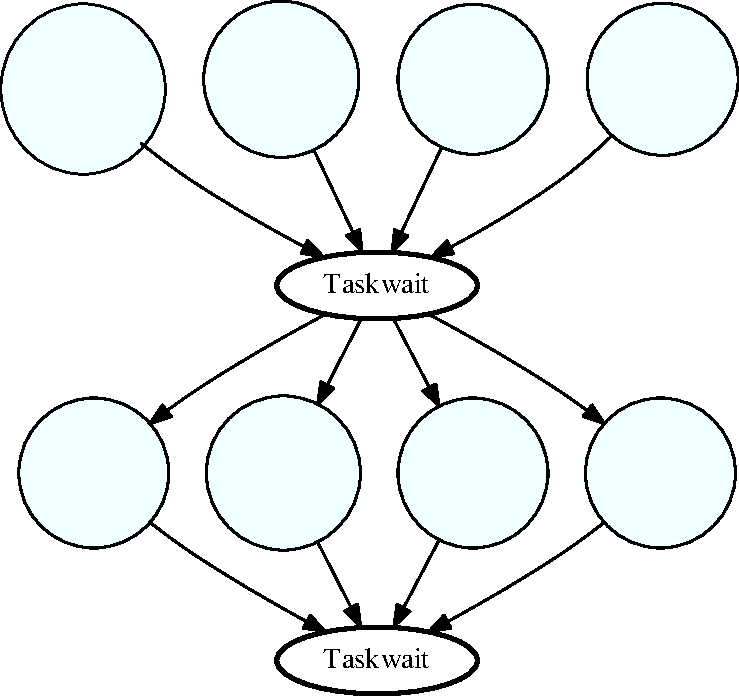
\includegraphics[width=0.5\columnwidth]{ifcg/figures/blackscholes_taskgraph}%
	\caption{Task-graph of blackscholes application.  No dependencies exit between tasks,
only barrier synchronization between iterations.}
	\label{fig:blackscholes_tg}%
	\vspace{.5cm}
\end{figure}

\paragraph{\textit{Pthreads}} This version simply divides the portfolio into
work units by the number of available threads, and stores them into the
\texttt{numOptions} array. Each thread calculates the prices for its
corresponding options and waits in a barrier until all the threads have
finished executing. The algorithm is run multiple times to obtain the final
estimation of the portfolio.


\paragraph{\textit{Task-based}} In the case of the task-based version, we
divide the work into units of a predefined block size. This block size allows
having much more task instances than threads, which implies a much better load
balance, as this is an embarrassingly parallel application with no dependencies
among tasks in the same run.  A task graph of the task-based implementation is
shown in figure \ref{fig:blackscholes_tg}.  We can see that this is an embarrassing
parallel application with only barrier synchronization between iterations of the 
main loop.  No data dependencies exist between tasks.
For all the task graphs shown in this document
we use smaller workloads than the ones used for evaluation.  This way it's easier
to read the task graphs.  For example in figure \ref{fig:blackscholes_tg} there are
four tasks per iteration, but this is easily configurable to hundreds or thousands 
of tasks.  Such is the case of the native workloads used for the evaluation of our 
implementations.



\begin{figure*}[ht!]
	\vspace{1cm}
	\centering
  \begin{subfigure}{0.9\textwidth}
		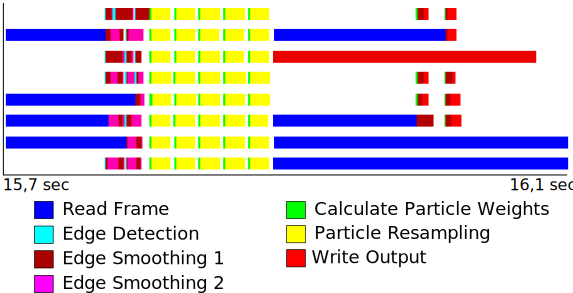
\includegraphics[width=\textwidth]{ifcg/figures/bodytrack-ompss-native-8-2dp_tasks_pthreads}
		\caption{Trivial Task-based Strategy}
	\label{fig:bodytrack-2dp_tasks-trace_pthreads}
  \end{subfigure}%
\\
\vspace{1cm}
\begin{subfigure}{0.9\textwidth}
		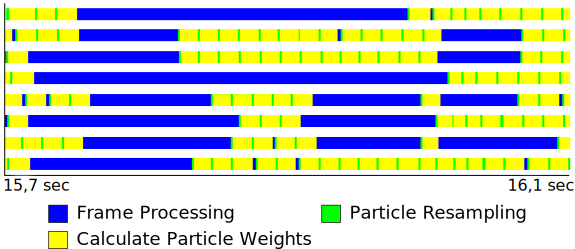
\includegraphics[width=\textwidth]{ifcg/figures/bodytrack-ompss-native-8-2dp_tasks_ompss}
		\caption{Optimal Task-based Strategy}
	\label{fig:bodytrack-2dp_tasks-trace_ompss}
  \end{subfigure}
	\caption{Parallel execution of Pthreads and task-based versions of \texttt{bodytrack} on an 8-core machine and native input size. Different parallel regions correspond to different colors.  White gaps in the figure, represent idle time.}%
	\label{fig:bodytrack-2dp_tasks-trace}%
\end{figure*}

\paragraph{\textbf{Bodytrack}}
Computer vision application that tracks a marker-less human body using multiple cameras
through an image sequence.  The application employs an annealed particle filter to track
the body using edges and the foreground silhouette as features of interest.

\begin{figure}[t!]%
	\center
	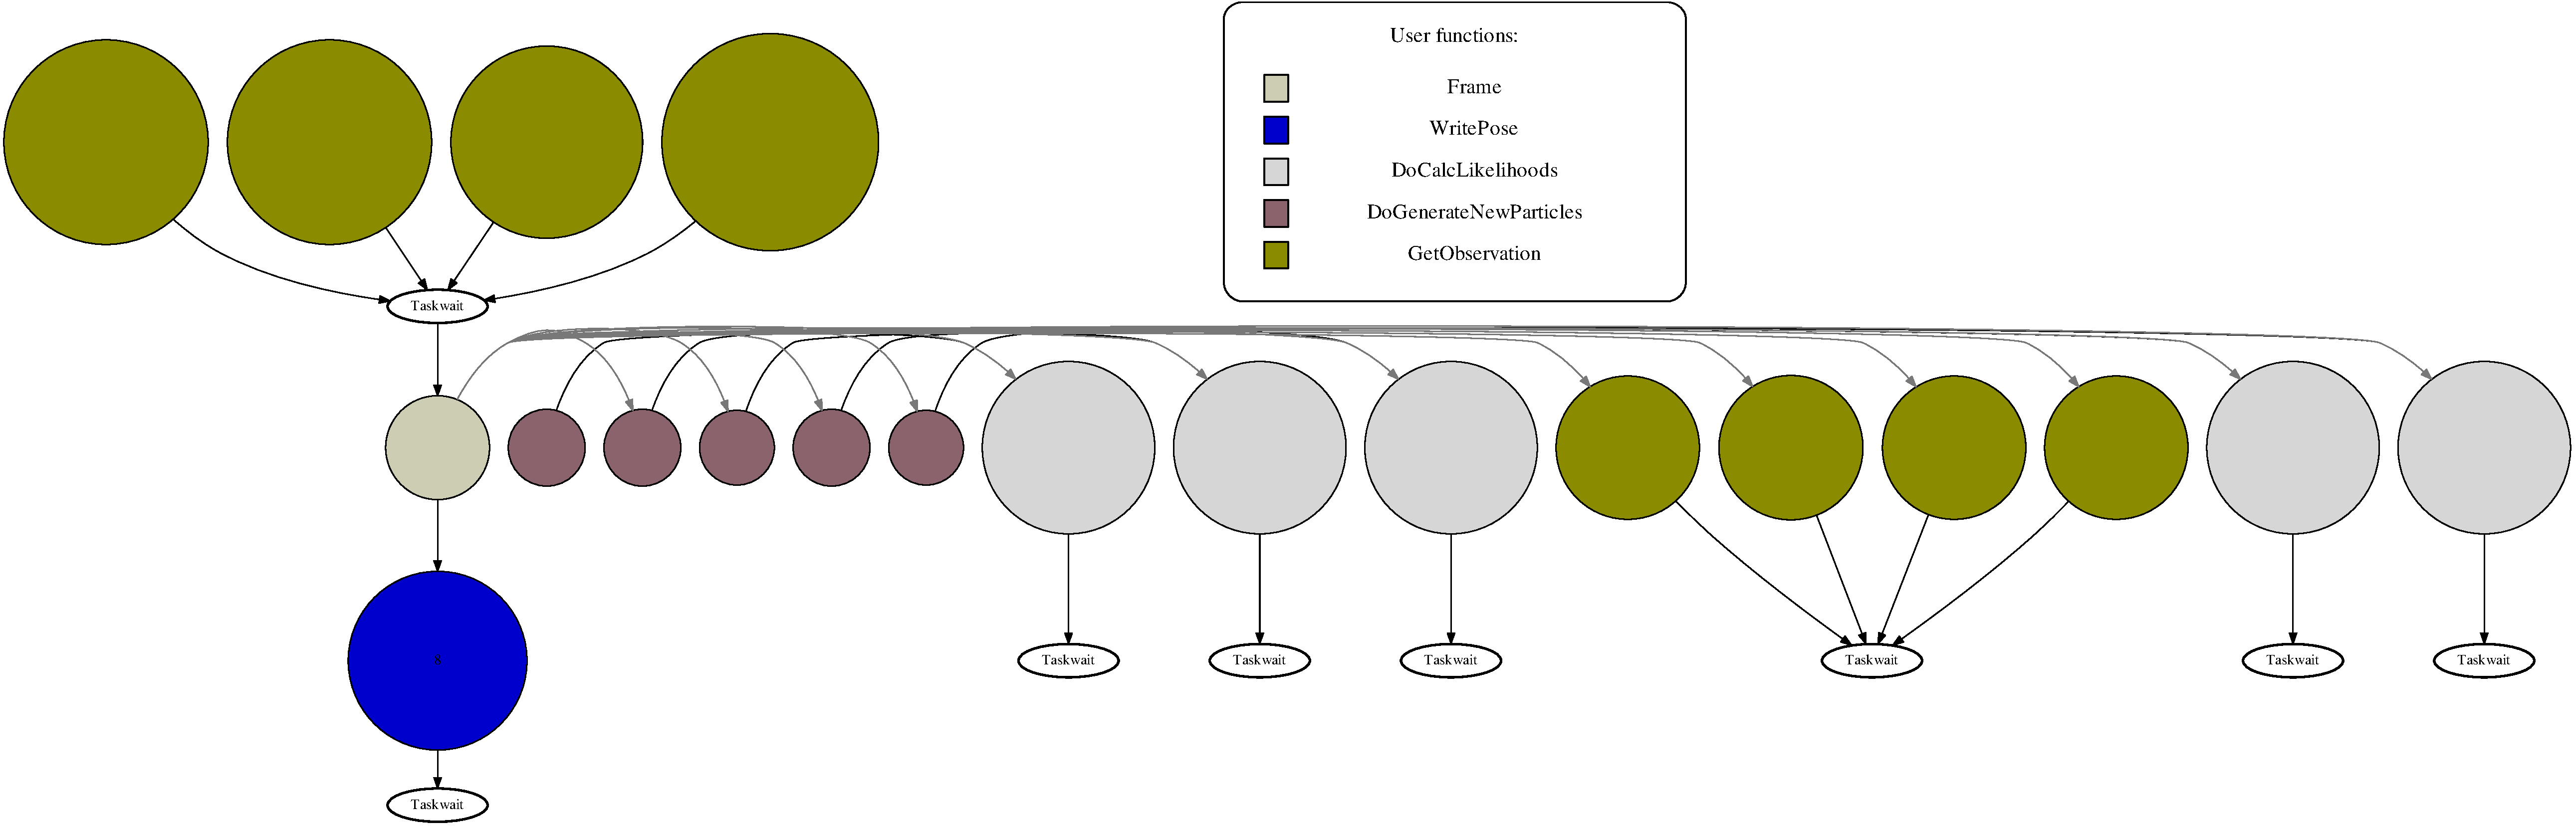
\includegraphics[width=\columnwidth]{ifcg/figures/bodytrack_taskgraph}%
	\caption{Task-graph of bodytrack application.  Edges show task data dependencies.}
	\label{fig:bodytrack_tg}%
	\vspace{.5cm}
\end{figure}



\paragraph{\textit{Pthreads}} \texttt{Bodytrack} applies the same algorithm on each frame
of the image sequence to track the different poses of the body.  The human body is modeled
as a tree-based structure, consisting of 7 conic cylinders.  It reads 4 images taken from
several cameras to capture a scene from 4 different angles, thus each frame consists of
these 4 images.  These images are read and encoded to a single data structure.  For each
frame, \texttt{bodytrack} extracts the edges and silhouette features for each of these 4
images.
In this feature extraction stage we have 3 different kernels.
\begin{enumerate}
	\item \textbf{Edge detection}: Gradient based edge detection.
	\item \textbf{Edge smoothing (phase 1)}: Gaussian filter used to smooth edges applied on array rows.
	\item \textbf{Edge smoothing (phase 2)}: Gaussian filter used to smooth edges applied on array columns.
\end{enumerate}
Afterwards, \texttt{bodytrack} goes through an annealed particle filter stage, which
consists of M annealing layers over a set of N particles.  The particles are multi-variate
configurations of the state and location of the tracked body.  Given the image features,
the particles are assigned weights, which increase or decrease the chance that a particle
represents a body part.  N particles are then chosen, depending on the probability
dictated by their weights.  Random noise is added to this set of particles, creating a new
set.  This process is repeated for all annealing layers. \texttt{Bodytrack} then picks one
of the M configurations, the one which has the highest weighted average.  This process has
two parallel kernels.
\begin{enumerate}[resume]
	\item \textbf{Calculate particle weights}: Computes weights for the particles, using the edges and silhouette produced from the previous stages.
	\item \textbf{Particle Resampling}: Adds Gaussian random noise to the particles, thus creating a new set of particles.
\end{enumerate}

In the case of Pthreads, the 4 images of a frame are read and processed in parallel using
one thread per image.  The Pthreads implantation is limited by the 4 images it can process
concurrently, while there is no other candidate work at this point.  A specific
asynchronous I/O implementation is required to read the files in parallel. Then, the
features extraction stage is executed using all the available threads, with a
synchronization barrier at the end of each phase. The same structure is followed in the
annealed particle filter stage, with two barriers at the end of each phase. Between the
two stages, serial code has to be executed, which leaves only one thread busy and the rest
idle.  Finally, the output results are written sequentially in one file.   


\paragraph{\textit{Task-based}} In the case of the task-based version, we adopt a more coarse grain approach. 
We do not parallelize the feature extraction stage, instead we 
taskify the whole frame processing, allowing concurrent execution of all frames. 
%Given enough frames to process, all threads can remain busy,
%which is not the case with the Pthreads version.
The parallel kernels of the annealed particle filter stage are taskified in our version, and synchronization is achieved
by dataflow annotations.  Figure \ref{fig:bodytrack_tg} shows a task graph of our implementation.  The directed edges show the
dependencies between the different tasks, which dictate the execution order of the tasks.
Each frame needs to be written when calculations are completed. In our version we can do this asynchronously while the threads are
busy with the processing stage of another frame.  Thus, output I/O is effectively overlapped with computation stages.


{Figure \ref{fig:bodytrack-2dp_tasks-trace} shows parallel executions of two different task-based implementations: 
The first one just mimics the Pthreads behavior (\ref{fig:bodytrack-2dp_tasks-trace_pthreads}) and the second is an optimal task-based implementation (\ref{fig:bodytrack-2dp_tasks-trace_ompss}).  
Different colored boxes represent different task types, as well the duration of that task type on each core. In both cases, the white gaps denote the time each thread spends idle.  
Both figures show the same duration for each execution. In the optimal version, all functionality is implemented within the frame-processing task, thus 
execution time for read-frame, edge-detection and edge-smoothing is represented with blue color (frame-processing).  
Tasks particle-resampling and calculate-particle-weights are also implemented as nested tasks. 
They are displayed with different colors (green and yellow respectively).  
We can observe that the Pthreads-like version suffers
from greater idle time compared to its optimal task-based counterpart. 
Work is distributed more efficiently in the optimal implementation
by processing different frames concurrently. 
This allows us to overlap I/O and serial code segments of one with available work from another one.
       
%To illustrate this point, Figure~\ref{fig:bodytrack-2dp_tasks-trace} shows an execution of \texttt{bodytrack} for two different frames. The x-axis represent time and the y-axis represent the cores where the execution takes place. 
%For example, a pixel of color blue in the (x,y) point means that at the instant x the core y is running the task codified by color blue. The red, dark red and green are tasks performing edge detection and edge smoothing, respectively.  
%The yellow color represents the task writing the output file. 
%Light green and magenta are the tasks that calculate particle weights and re-sample the particles. Light blue color annotates the idle time or sequential code execution. 
%%
%We can see how the task that writes the output file for frame N-1 (in yellow) is overlapped by the three first computation tasks of frame N, which does not happen in the Pthreads version of the code.
%This overlapping is the main source of performance gains archived by using the dataflow task-based paradigm with \texttt{bodytrack}. 
%Section~\ref{sec:evaluation} reports these improvements in detail.

\paragraph{\textbf{Canneal}}
This kernel uses a cache-aware simulated annealing~\cite{Banerjee:1994:PAV:185340} to
optimize routing cost of a chip design.  \texttt{Canneal} progressively swaps elements
that need to be placed in a large space, eventually converging to an optimal solution. The
problem is stored as a list with routing costs between nodes. 

\begin{figure}[t!]%
	\center
	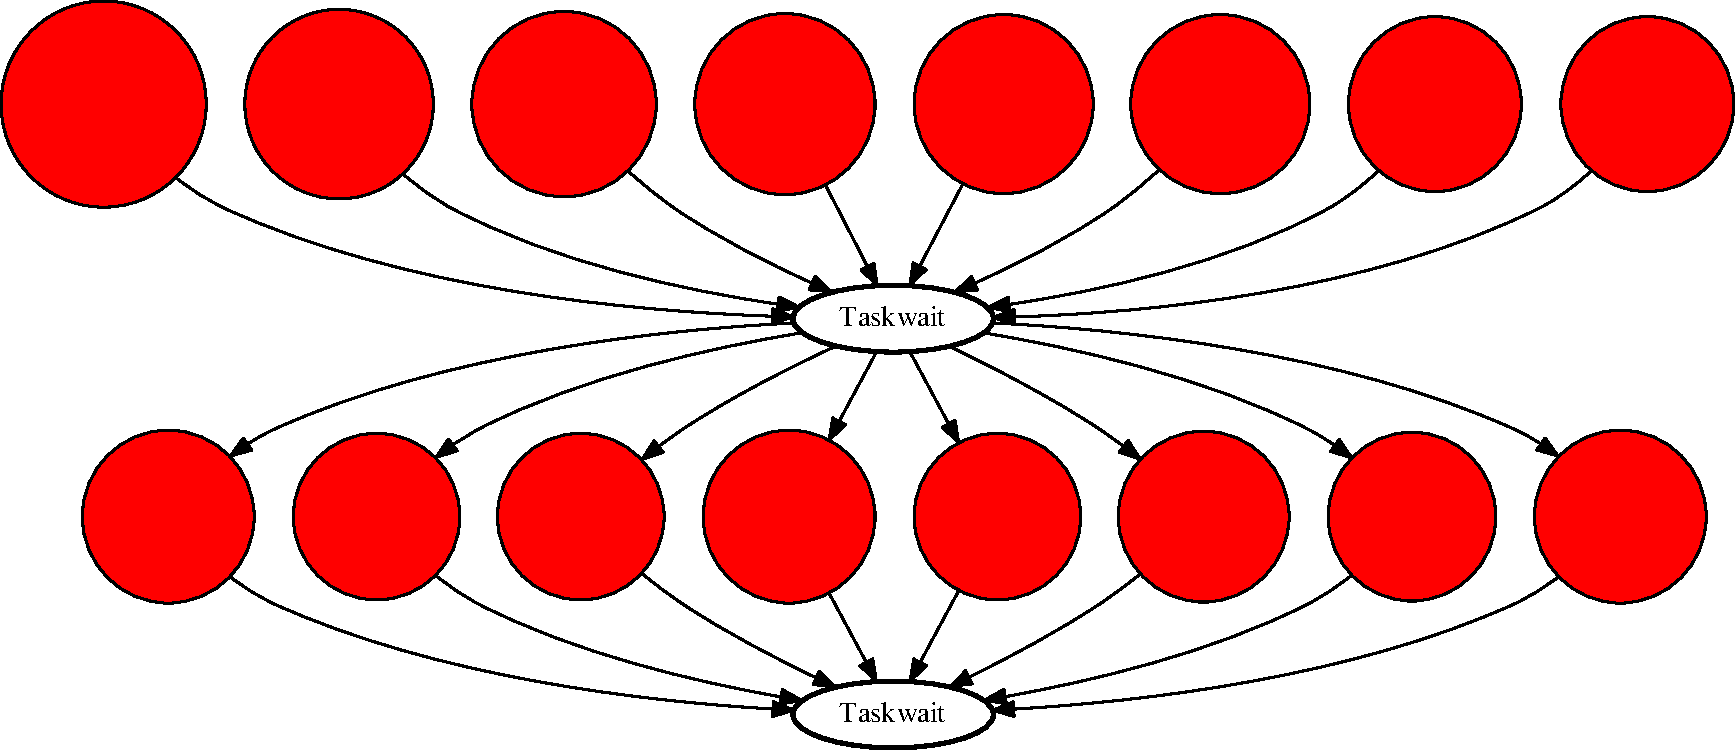
\includegraphics[width=.8\columnwidth]{ifcg/figures/canneal_taskgraph}%
	\caption{Task-graph of canneal application.  Only barrier synchronization among tasks.}
	\label{fig:canneal_tg}%
	\vspace{.5cm}
\end{figure}

\paragraph{\textit{Pthreads}} This version compares random element pairs of the graph
concurrently and swaps them until it converges to an optimal solution.  No locks are used
to protect the list from concurrent accesses/writes, but  swaps are done atomically
instead. However, the evaluation of the elements to be swapped is not atomic.  This means
that disadvantageous swaps may occur, which will require the algorithm to eventually swap
them again.  This method has provided better results than the alternative algorithm with
locks~\cite{bienia2008}.

\paragraph{\textit{Task-based}} Our task-based version follows the same paradigm.  Several
tasks are spawned without any dependencies between themselves. We use the same atomics as
with the Pthreads version.  Since tasks work with an arbitrary number of list elements, it
is not possible to describe which elements of the list a task is going to randomly access. 
In the task graph in figure \ref{fig:canneal_tg} it is clear that there are no data dependencies.
Synchronization is only achieved through the use of barriers.

We also try an alternative fine grain implementation, where a task is spawned for each
random pair of list elements.  This would allow the runtime to know if two tasks are
working on the same list of elements. However this implementation implied fine-grain
tasks. Each task would merely do a single swap between two list elements.  The overhead of
the dynamic scheduling is a problem in this scenario.  A more complex but more efficient
solution is suggested by Symeonidou et al.~\cite{Symeonidou:2013:DDR:2488551.2488558} with
the use of memory regions.  Adopting this method in a task-based model would allow the
programmer to describe parts of the list (or other pointer based data structures) and
express dataflow relations as abstract memory regions.  This solution also implies
fine-grain tasking and is not evaluated at the Symeonidou's work. 

\begin{figure}[t!]%
	\center
	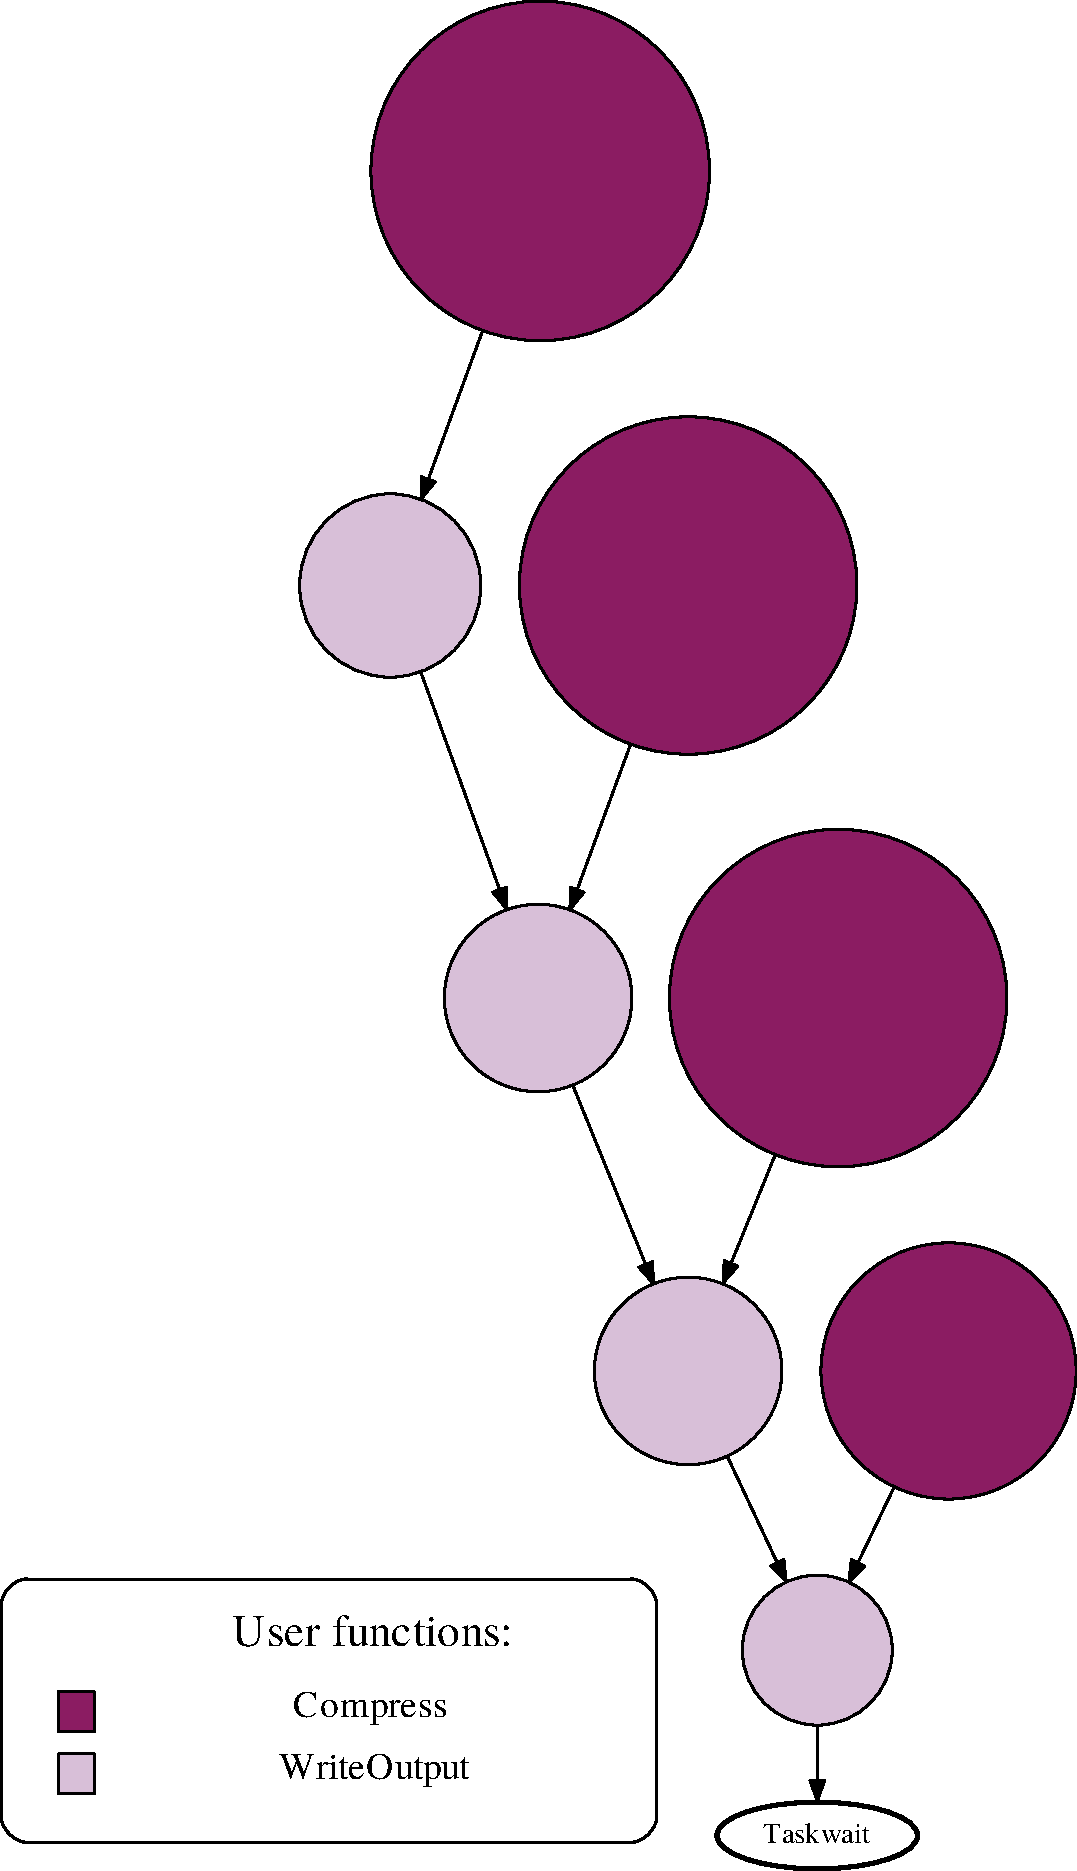
\includegraphics[width=.4\columnwidth]{ifcg/figures/dedup_taskgraph}%
	\caption{Task-graph of dedup application.  Data dependency edges force the correct order
of writting the data chunks to the output.}
	\label{fig:dedup_tg}%
	\vspace{.5cm}
\end{figure}


\paragraph{\textbf{Dedup}}
The \texttt{dedup} kernel is used to compress data streams using local and global
compression to achieve higher compression rates.  This method is called
deduplication~\cite{Quinlan:2002:ABP:1083323.1083333}.

\paragraph{\textit{Pthreads:}}
Dedup is parallelized using a pipeline model with the following stages:
\begin{itemize}
  \item \textbf{Fragment}:  First, the data-stream is read and partitioned at fixed positions into coarse grain data chunks. Each chunk can be processed individually by the rest of the stages. This stage is executed on a single thread.
  \item \textbf{Fragment Refine}:  A new data chunk initiates the second pipeline stage, where it is further partitioned into smaller fine-grain
	chunks.  The portioning is done by using the Rolling-fingerprint algorithm.  
  \item \textbf{Deduplication}:  This stage eliminates duplicate fine-grain chunks.  Unique chunks are stored in a hash-table.
	Locks are used here to protect	each bucket from concurrent accesses.
  \item \textbf{Compress}:  At this stage chunks are compressed in parallel.  Identical chunks are compressed only once as duplicates are removed 
	at the deduplication stage.
  \item \textbf{Reorder}:  This stage writes the final compressed output data to a file.  It writes only unique chunks' compressed data and for the
	duplicates it stores their hash values.  However this stage needs to reorder the data chunks as they are received
	to match the original order of the uncompressed data.
\end{itemize}

The Pthreads version maintains a queue and a thread pool dedicated to each stage.  When a
chunk becomes available at one stage, it is moved to the queue of the next stage.  Each
stage polls at its queue for available chunks to process. The reorder stage is done
sequentially with a devoted thread that can be in an idle loop waiting for previous stages
to finish.  Each thread pool  comprises by a number of threads equal to the number of
available cores.  The only exceptions are \texttt{Fragment} and \texttt{Reorder} stages,
which are served by a single thread each.

%\begin{figure}[ht!]%
%	\centering
%	\begin{lstlisting}
%void Fragment{
%  ...
%  while ( chunk = read_bytes() ) {
%		chunks[nCChunks][0] = chunk;
%		#pragma omp task inout(chunks[nCChunks]) 
%		Fragment(chunks[nCChunks]);
%		#pragma omp task inout(chunks[nCChunks])
%		WriteOutput(outfile, chunks[nCChunks]);
%		nCChunks++;
%		break;
%  }
%  #pragma omp taskwait
%	...
%}
%	\end{lstlisting}
%	\caption{Dedup task-based implementation pseudocode of the \texttt{Fragment} stage.}%
%	\label{lst:dedup-ompss}%
%\end{figure}

\begin{figure}[!t]%
	\centering
	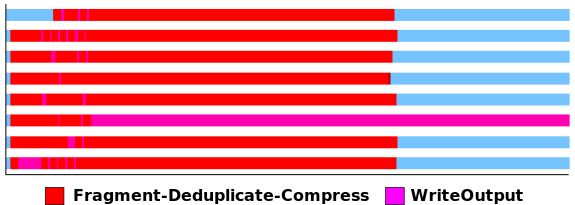
\includegraphics[width=0.9\columnwidth]{ifcg/figures/dedup-ompss-native-8-2dp_tasks}%
	\caption{Parallel execution of the task-based version of \texttt{dedup} on an 8-core machine and native input size. Different task types correspond to different colors.}%
	\label{fig:dedup-2dp_tasks-trace}%
	\vspace{.5cm}
\end{figure}


\paragraph{\textit{Task-based}}
In our implementation we taskify each pipeline stage and express data dependencies using static arrays and dataflow relations, one for each pipeline stage.
\texttt{FragmentRefine} however partitions the data chunks into very fine grain segments, ranging from a few hundreds to thousands. For such granularity,
our approach suffers from high overheads due to dynamic schedulnig overhead. 
The same is observed in~\cite{Vandierendonck:2013:DSP:2503210.2503233}, where 
an alternative approach is adopted. In their approach, two pipelines are identified: The outer pipeline, consisting of stages \texttt{Fragment}, \texttt{InnerPipeline}
and \texttt{Reorder}. The inner pipeline consists of \texttt{FragmentRefine}, \texttt{Deduplicate} and \texttt{Compress}.  To reduce the dynamic scheduling overhead,
they merge together \texttt{Deduplicate} and \texttt{Compress}. By doing so, the available parallelism is limited, but still there is enough work not to harm performance
and scalability. In our approach, we merge together the inner pipeline, creating one sequential function, exploiting only the parallelism available in the outer pipeline.
Even in this scenario, the available parallelism is still abundant, since the application is bound by the writing of the output file, which is sequential.  
Figure~\ref{fig:dedup-2dp_tasks-trace} shows a trace of the task-based version.  We can see that communication stage (in yellow) is effectively overlapped with the computation stage (in red), however,
there is not enough work to keep all the threads finish, until the end of the execution.

Furthermore, we modify the \texttt{Reorder} stage, by replacing it with a simple stage where the chunk is simply written to file (\texttt{WriteOutput}).
Using dataflow relations and a shared output resource between the \texttt{WriteOutput} tasks, we ensure that chunk \texttt{N-1} will be written before chunk \texttt{N}. 
Thus, we do not need to reorder data chunks in this task type.  Moreover, the scheduler makes sure chunks are written as soon as they become available by the \texttt{InnerPipeline} task, an improvement
over the Pthreads version, where \texttt{Reorder} instances need to idle wait until all previous chunks ones have been written.  
Figure \ref{fig:dedup_tg} shows the dependencies among tasks.  We can observe that \texttt{WriteOutput} tasks will be run in the correct
order, as soon as their dependencies are resolved.
Another difference between the two versions, is that Pthreads 
oversubscribe threads to cores for each pipeline stage, while in our implementation we only assign one thread to each core.


\paragraph{\textbf{Facesim}}
Computes a visually realistic human face animation by simulating the underlying physics.  As input it uses a 3D model of a human face 
containing both a tetrahedra mesh and triangulated surfaces for the flesh and bones, respectively. Additionally it uses 
a time sequence of muscle movement \cite{Sifakis:2005:ADF:1073204.1073208}.

\paragraph{\textit{Pthreads}}
The application statically decomposes the original tetrahedron mesh into smaller partitions, equal to the number of available threads.
%The boundaries of the partitions are replicated to avoid synchronization. The trade-off is redundant computations. For the bones, they 
%are employed serially. 
There are three main parallel kernels:
\begin{itemize}
  \item \textbf{Update State}: Calculates the steady properties of the mesh, constrains like stress and stiffness.  
%This is done by solving a nonlinear system of equationsusing the Newton-Rhapson method.  
  \item \textbf{Add Forces}: Computes the force contribution between vertices acting on the 3D model.
  \item \textbf{Conjugate Gradient (CG)}:  An iterative method that solves the linear system produced by the 
other two previous kernels and find the final displacement of the vertices for the current frame.
\end{itemize}

\texttt{Update\_State} and \texttt{Add\_Forces} kernels consist of one and two parallel loops respectively, while \texttt{CG} has three. 
Synchronization between loops and kernels is achieved by barriers.  The corresponding force computations from the skeleton are also done 
in \texttt{Update\_State} and \texttt{Add\_Forces}, but after the parallel computations on the tetrahedra mesh have been made. 
In Pthreads a master thread is assigning work to all threads in a round-robin fashion through a queuing system.  Each thread maintains 
its private queue, which is protected by locks.

%\begin{figure}[!t]%
%	\centering
%	\includegraphics[width=0.8\columnwidth]{figures/facesim-ompss-native-8-2dp_tasks}%
%	\caption{Parallel execution of the task-based version of \texttt{facesim} on an 8-core machine while simulating a frame. 
%	Different task types correspond to different colors, while idle time is represented in light blue color.}%
%	\label{fig:facesim-2dp_tasks-trace}%
%\end{figure}

\paragraph{\textit{Task-based}}
In the task-based version, the application level queuing system is completely replaced by the OmpSs runtime.  In our initial implementation 
all parallel loops are taskified. 
Additionally,  in \texttt{Update\_State} there is a sequential code segment, 
\texttt{Update\_Collision\_Penalty\_Forces}.  
This code segment operates on the bones, while the parallel loop of \texttt{Update State} does so on the tetrahedra.  
By taskifying it and adding dataflow relations between this Section and the following \texttt{Add\_Forces} kernel, we can overlap 
\texttt{Update\_Collision\_Penalty\_Forces} with the rest of \texttt{Update\_State}.


%\edit{In the \texttt{CG} kernel, we managed to remove two out of three barriers, which synchronized the different parallel loops, by using dataflow relations 
%to describe data dependencies.  One barrier could not be removed as it protects the residual calculation at theend of each iteration of the solver, 
%whose value is used to control whether we exit the loop or not.}  
%\edit{This initial implementation suffered from high task creation time in the \texttt{CG} kernel.  Note that this is an issue of OmpSs' runtime, out OpenMP 4.0 task implementation 
%did not manifest this issue.}
To improve performance we refactor tasks' creation in \texttt{CG} by nesting the first task creation loop inside another task.
This enables us to overlap task creation time with computation, which contributes to increase \texttt{Facesim's} task-based implementation performance.  
Although we achieve better scalability than the original code, task creation still imposed overheads. To address this issue
we replace tasks in \texttt{CG} with the OmpSs parallel loops construct (equivalent to the OpenMP one), which implements loop worksharing 
with a task. Even though this approach limits the available parallelism (barrier synchronization, no dataflow annotations), the overhead 
associated to task creation and scheduling is greatly reduced and overall performance improved.

\paragraph{\textbf{Ferret}}
Content similarity search server for feature-rich data~\cite{Lv:2006:FTC:1218063.1217966} like audio, video, images, etc.
The benchmark application is configured for image similarity search.  
%\begin{figure}[t!]%
%	\begin{lstlisting}
%void load() {
%	int i = 0;
%	while( load_image(image[i]) ) {
%		#pragma omp task in(image[i]) out(seg_images[i])
%		seg_images[i] = t_seg(image[i]);
%		#pragma omp task in(seg_images[i]) out(extract_data[i])
%		extract_data[i] = t_extract(seg_images[i]);
%		#pragma omp task in(extract_data[i]) out(vectoriz_data[i])
%		vectoriz_data[i] = t_vec(extract_data[i]);
%		#pragma omp task in(vectoriz_data[i]) out(rank_results[i])
%		rank_results[i] = t_rank(vectoriz_data[i]);
%		#pragma omp task in(rank_data[i]) out(outstream)
%		t_out(rank_data[i], outstream);
%		i++;
%	}
%	#pragma omp taskwait
%}
%	\end{lstlisting}
%	\caption{Ferret ompss implementation}%
%	\label{lst:ferret-ompss}%
%\end{figure}

\begin{figure}[t!]%
	\center
	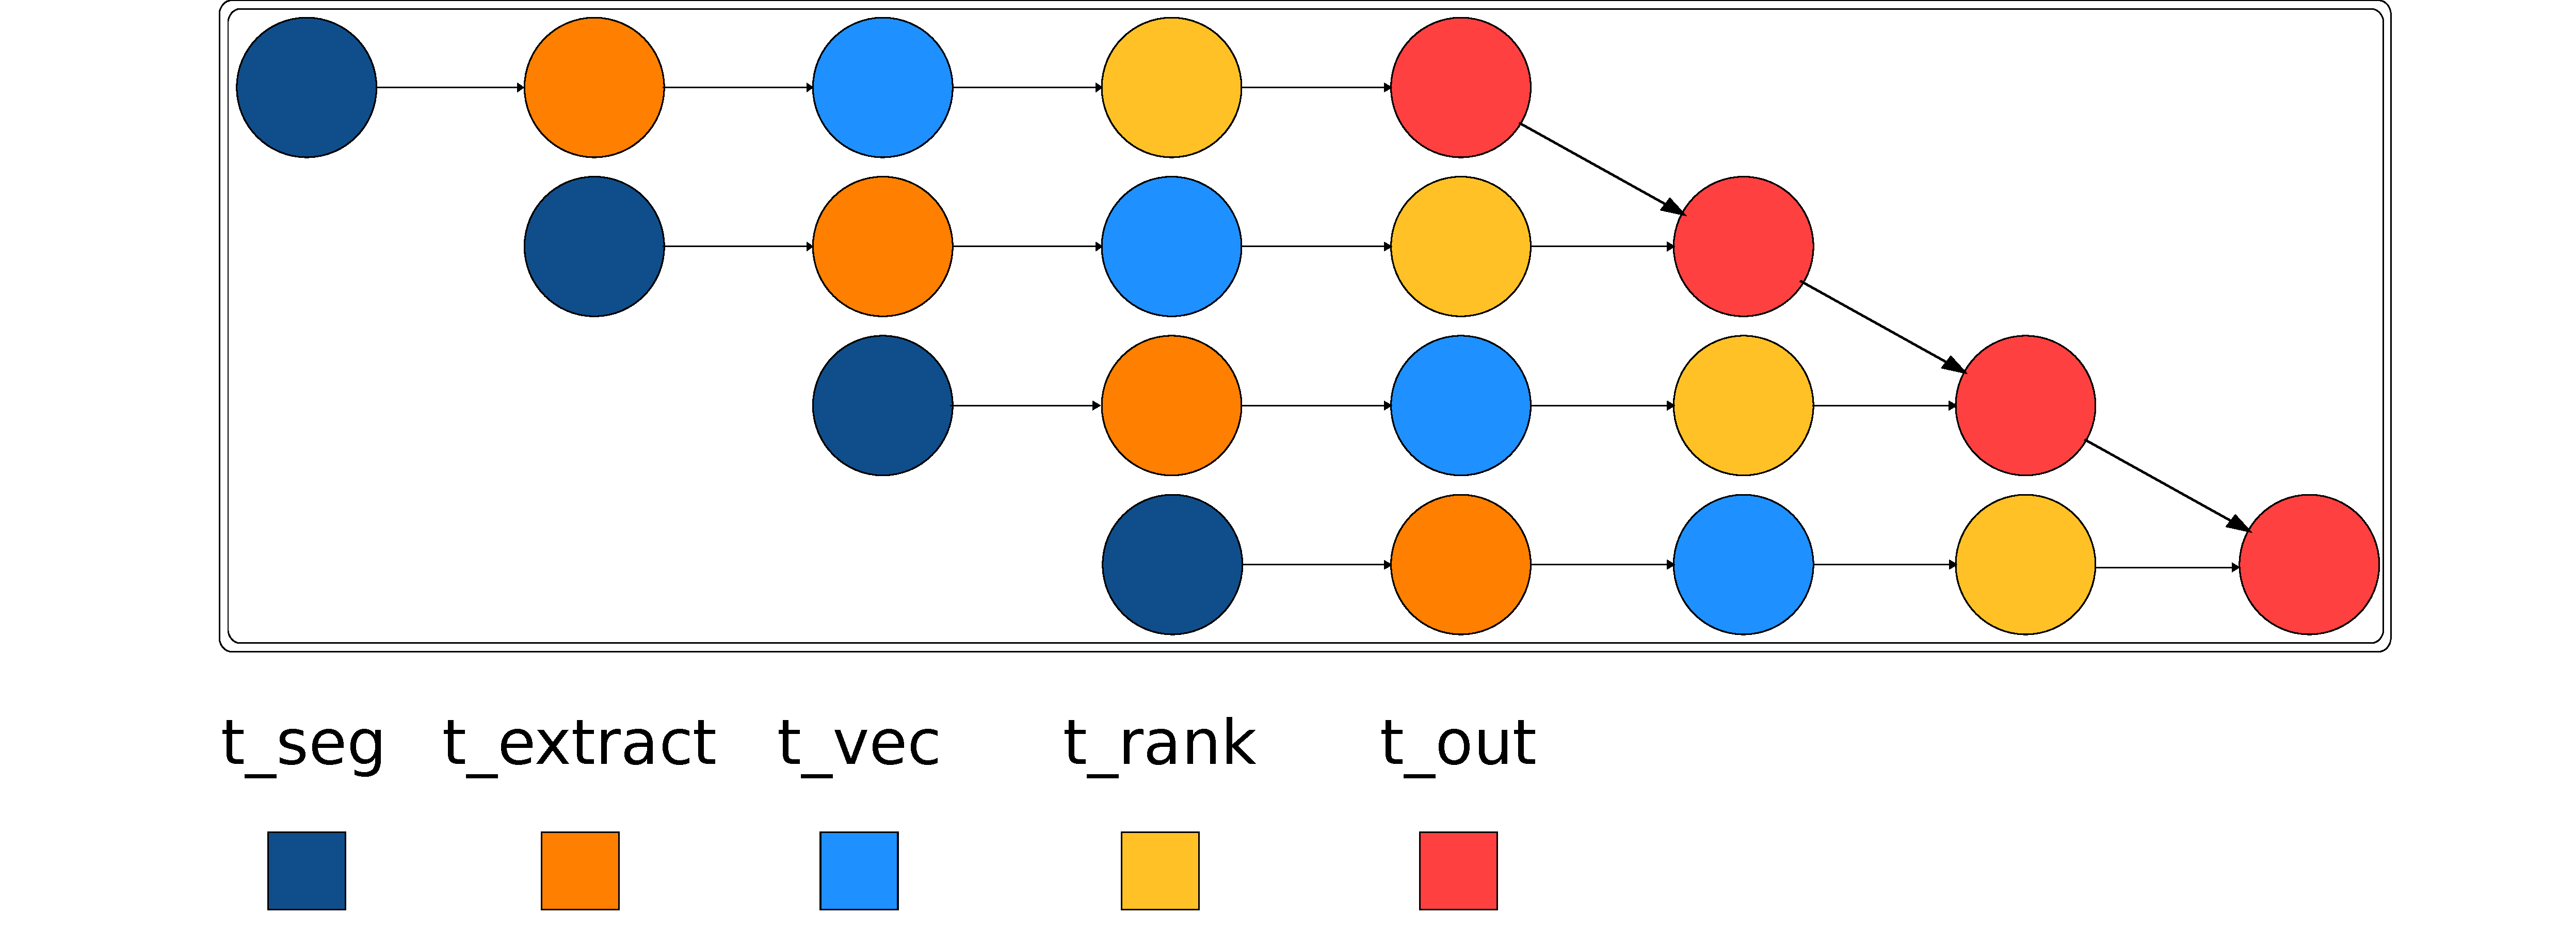
\includegraphics[width=0.9\columnwidth]{ifcg/figures/ferret_tg}%
	\caption{Task-graph of ferret showing the pipelined execution model.  Edges show data dependencies among different tasks.}
	\label{fig:ferret_tg}%
	\vspace{.5cm}
\end{figure}

\paragraph{\textit{Pthreads}}
Ferret is parallelized using a pipeline model.  A serial query is broken down into 
6 pipeline stages:
\begin{itemize}
  \item \textbf{Load}:  This stage loads an image that is going to be used as a query.
  \item \textbf{Segmentation}:  At this stage the image is decomposed into the different objects displayed on it.
	Different weight vectors are to be assigned on each object to achieve better results.
%	For example if an object is identified as a background it will have a smaller weight
%	than other objects.
  \item \textbf{Extract}:  At this stage a 14-dimensional vector is computed for each object from the segmentation stage, 
														describing features such as color, area, state, etc.
  \item \textbf{Vectorization}:  This is the indexing stage that tries to find a set of candidate images in the database.
  \item \textbf{Rank}:  This stage ranks the results found, using the EMD metric for each query-object's vector
	and the database's image vectors.
  \item \textbf{Output}:  Outputs the result of the ranking stage.  Multiple instances of
	this stage need to run serially, since they all share the same output stream.

\end{itemize}

In the Pthreads version every stage is served by a dedicated thread-pool of N threads each, where N is the number of available cores.
The only exceptions are the \texttt{Load} and \texttt{Output} stages that are executed by a respective single thread.
Each stage polls on its corresponding queue for available work.  When a stage finishes,
it pushes the results to the next stage's queue. 

\paragraph{\textit{Task-based}}
In this version, we implement a variation of this pipeline model. As soon as the first
stage, \texttt{Load}, finds a new image, it spawns all stages of a pipeline for that
image, thus reducing the pipeline to five stages.  We model the dataflow relations between
different stages as simple one dimension arrays, as shown in
Figure~\ref{lst:ferret-ompss}.  Tasks working on different image queries do not share any
dependencies. An exception is task \texttt{t\_out} which shares the same output file
between all pipelines, thus sequential execution is forced between all instances of this
task.  The pipeline stages and dependencies are constructed a priori, which is good enough
for this application, but this is not always the case.
\cite{Lee:2013:OPP:2486159.2486174} proposes a system that can handle dynamic pipeline
creation by constructing a DAG with the stages using indexes and the
\texttt{cilk\_continue} and \texttt{cilk\_wait} keywords.  Indexes are used to define the
different pipeline stages, while \texttt{cilk\_continue} creates a stage that can run once
all previous stages in the same pipeline iteration are done, and \texttt{cilk\_wait}
creates a stage that will wait for its stage counterpart of the previous iteration to
finish.  A strategy based on versioning the dependency objects between the stages has been
proposed~\cite{Vandierendonck:2011:PPG:2001252.2001265}.  Output dependencies are renamed
and privatized, thus the static array for privatization is not required.  

Figure \ref{fig:ferret_tg} shows the task-graph of the \texttt{ferret} application.
Colored nodes denote the concurrent tasks (each color matches a specific task type).
Tasks that have data dependencies are connected by directed edges.  By inspecting the
task-graph we can see a pipeline pattern of execution.  Despite the fact that the
task-based approach does not significantly improve the overall performance, as we can see
in Section~\ref{sec:task_bench_evaluation}, it significantly reduces the effort required
to express the pipeline parallelism, compared its Pthreads counterpart, as it is shown in
Section~\ref{sec:lines} in detail.


\paragraph{\textbf{Fluidanimate}}
This application simulates incompressible fluid interactive animation, using the 
Smoothed Particle Hydrodynamics (SPH) method~\cite{Muller:2003:PFS:846276.846298}.

\begin{figure}[t!]%
	\center
	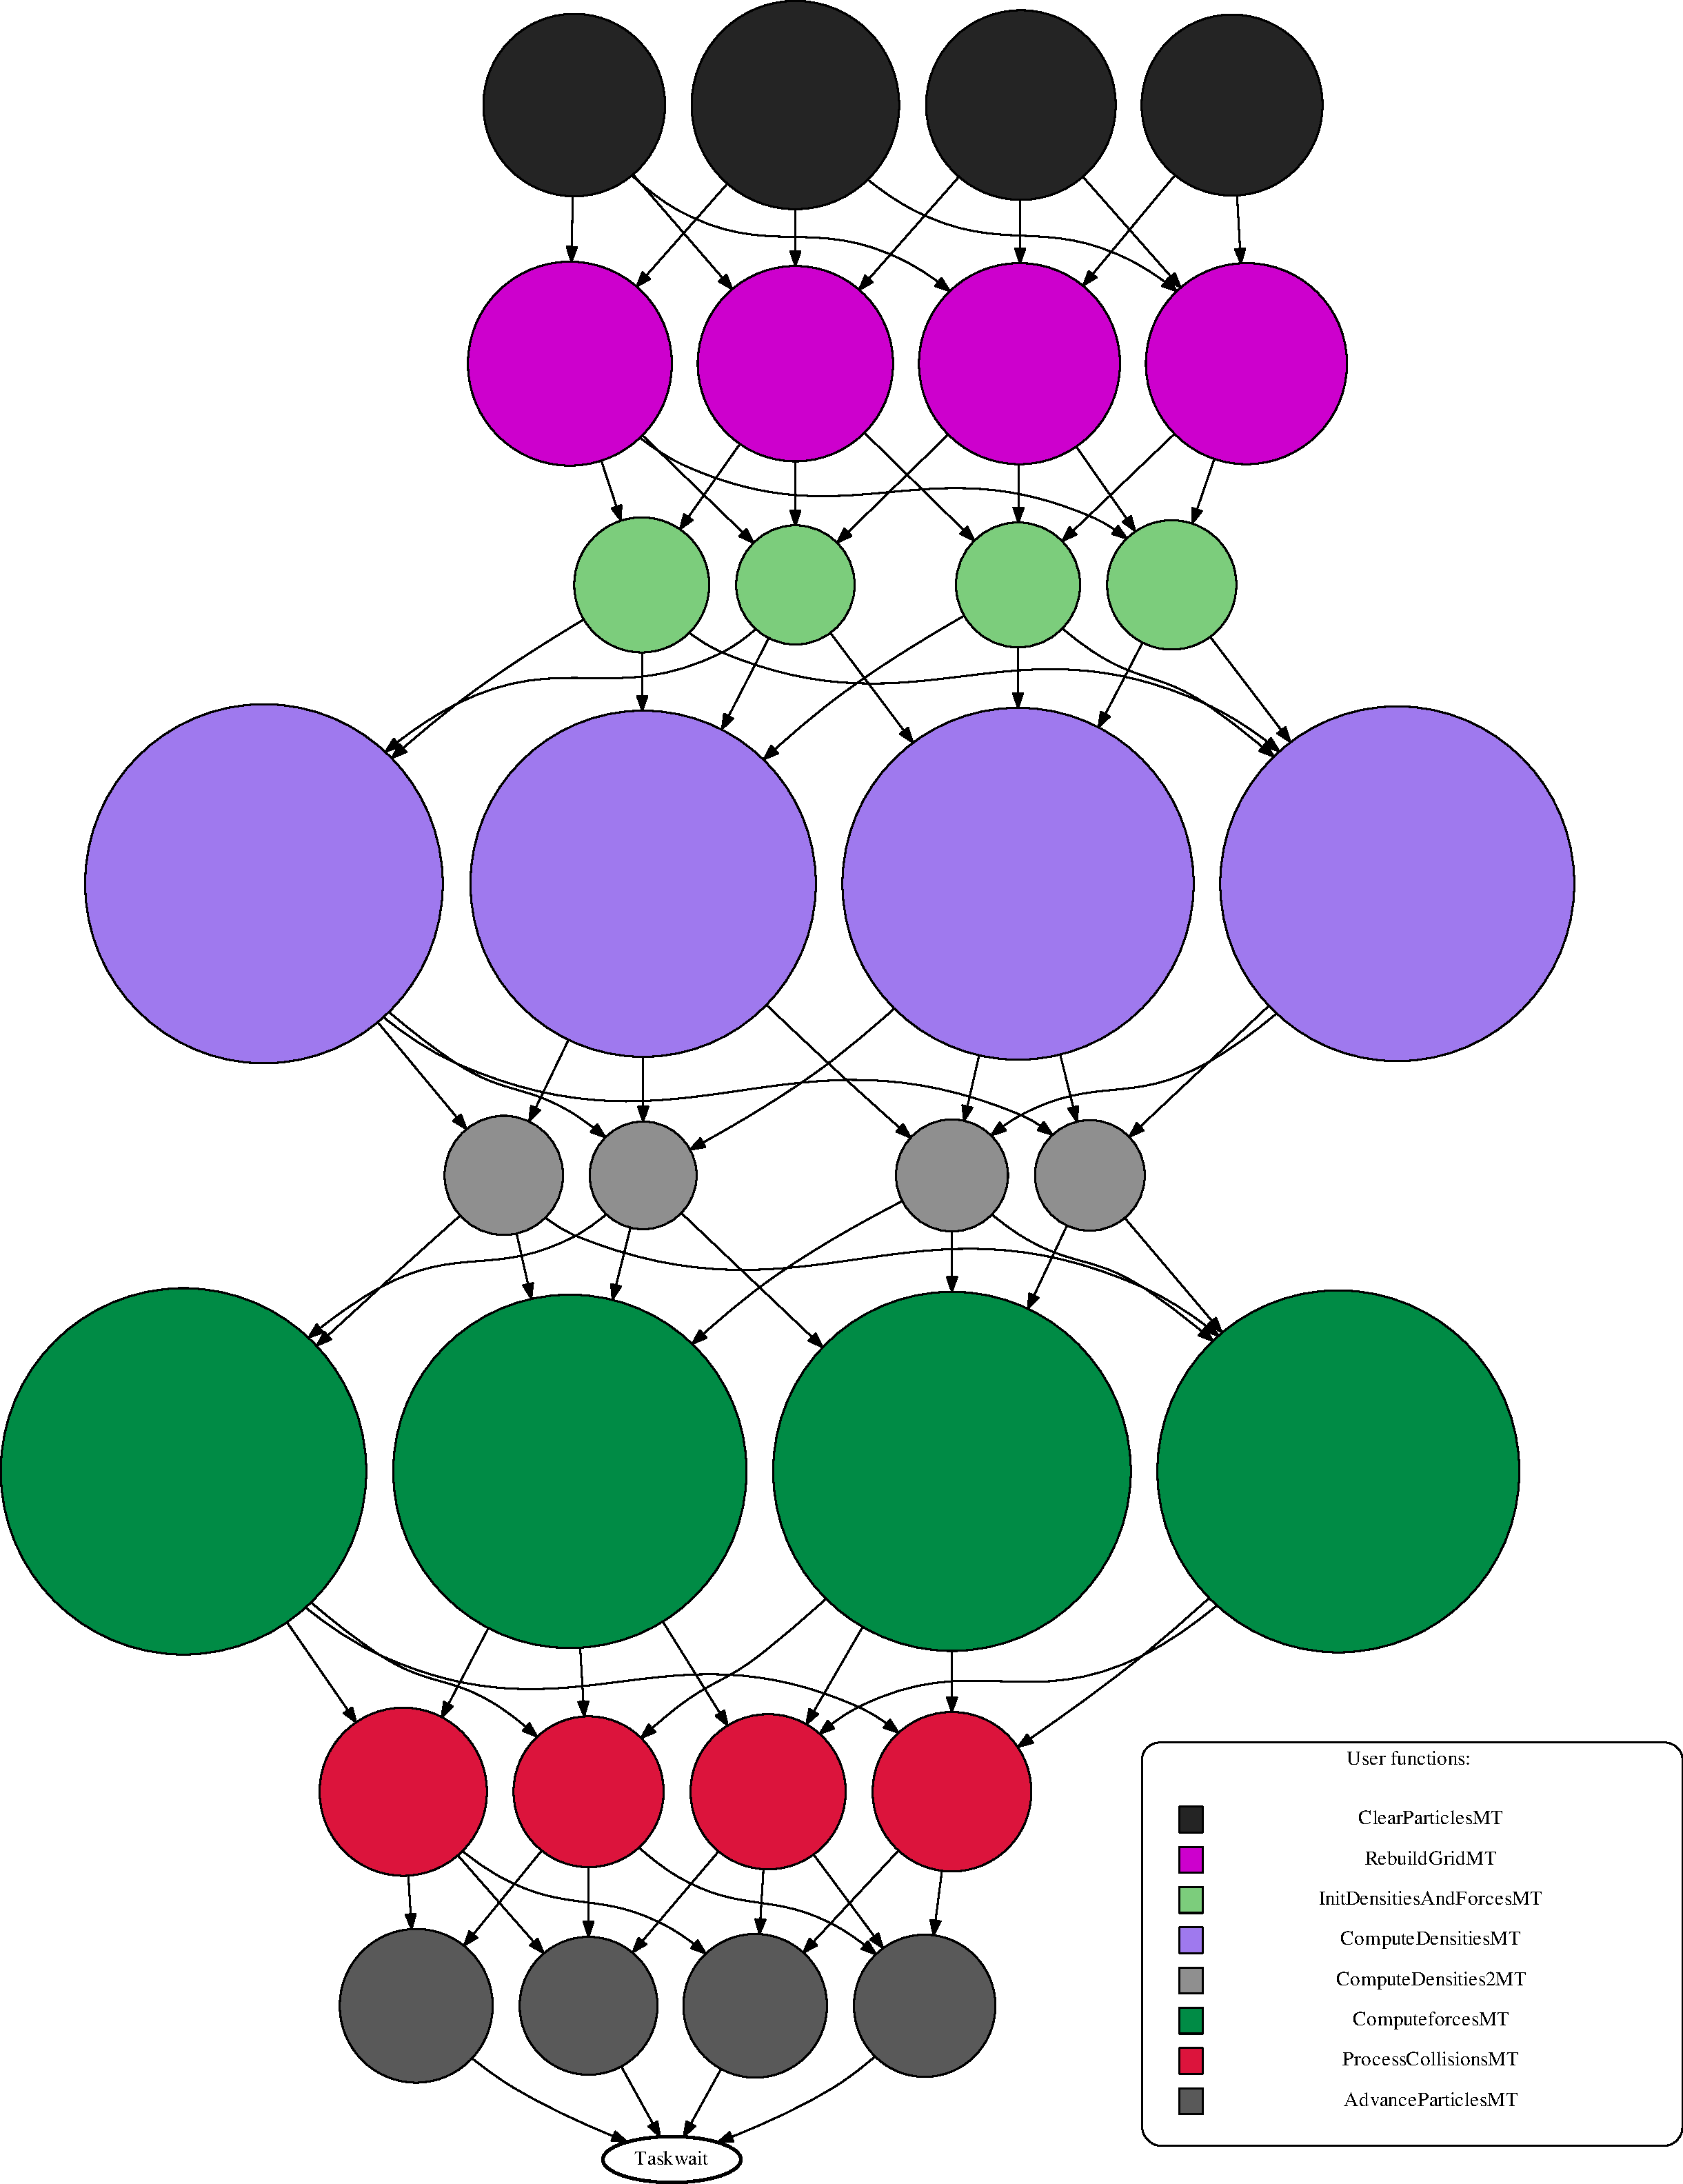
\includegraphics[width=.6\columnwidth]{ifcg/figures/fluidanimate_taskgraph}%
	\caption{Task-graph of fluidanimate application. Edges represent data dependencies among
tasks}
	\label{fig:fluidanimate_tg}%
	\vspace{.5cm}
\end{figure}

\paragraph{\textit{Pthreads}}
\texttt{Fluidanimate} uses five special kernels which are responsible for rebuilding the
spatial index, computing fluid densities and forces at given points, handling fluid
collisions with the scene geometry and finally updating particle locations The fluid
surface is partitioned and each thread works on its own grid segment.  The kernels are
parallelized as do-all loops, separated by barriers. Moreover, there are cases where these
threads need to update values beyond their partition, which are handled using locks.

\paragraph{\textit{Task-based}}
The task-based implementation follows the same approach, we apply a loop tiling
transformation, for each parallel loop, and taskified each iteration.  
Figure \ref{fig:fluidanimate_tg} show how dependencies form among between tasks.  
Tasks from different loops can run concurrently, as soon as their dependencies are met.
For example we see that the first task of each loop, only requires that the first two tasks
from the previous loop finish their execution to have their dependencies resolved.
We maintain the
same barrier and lock synchronization scheme, using the OmpSs synchronization primitives.

\begin{figure}[t!]%
	\center
	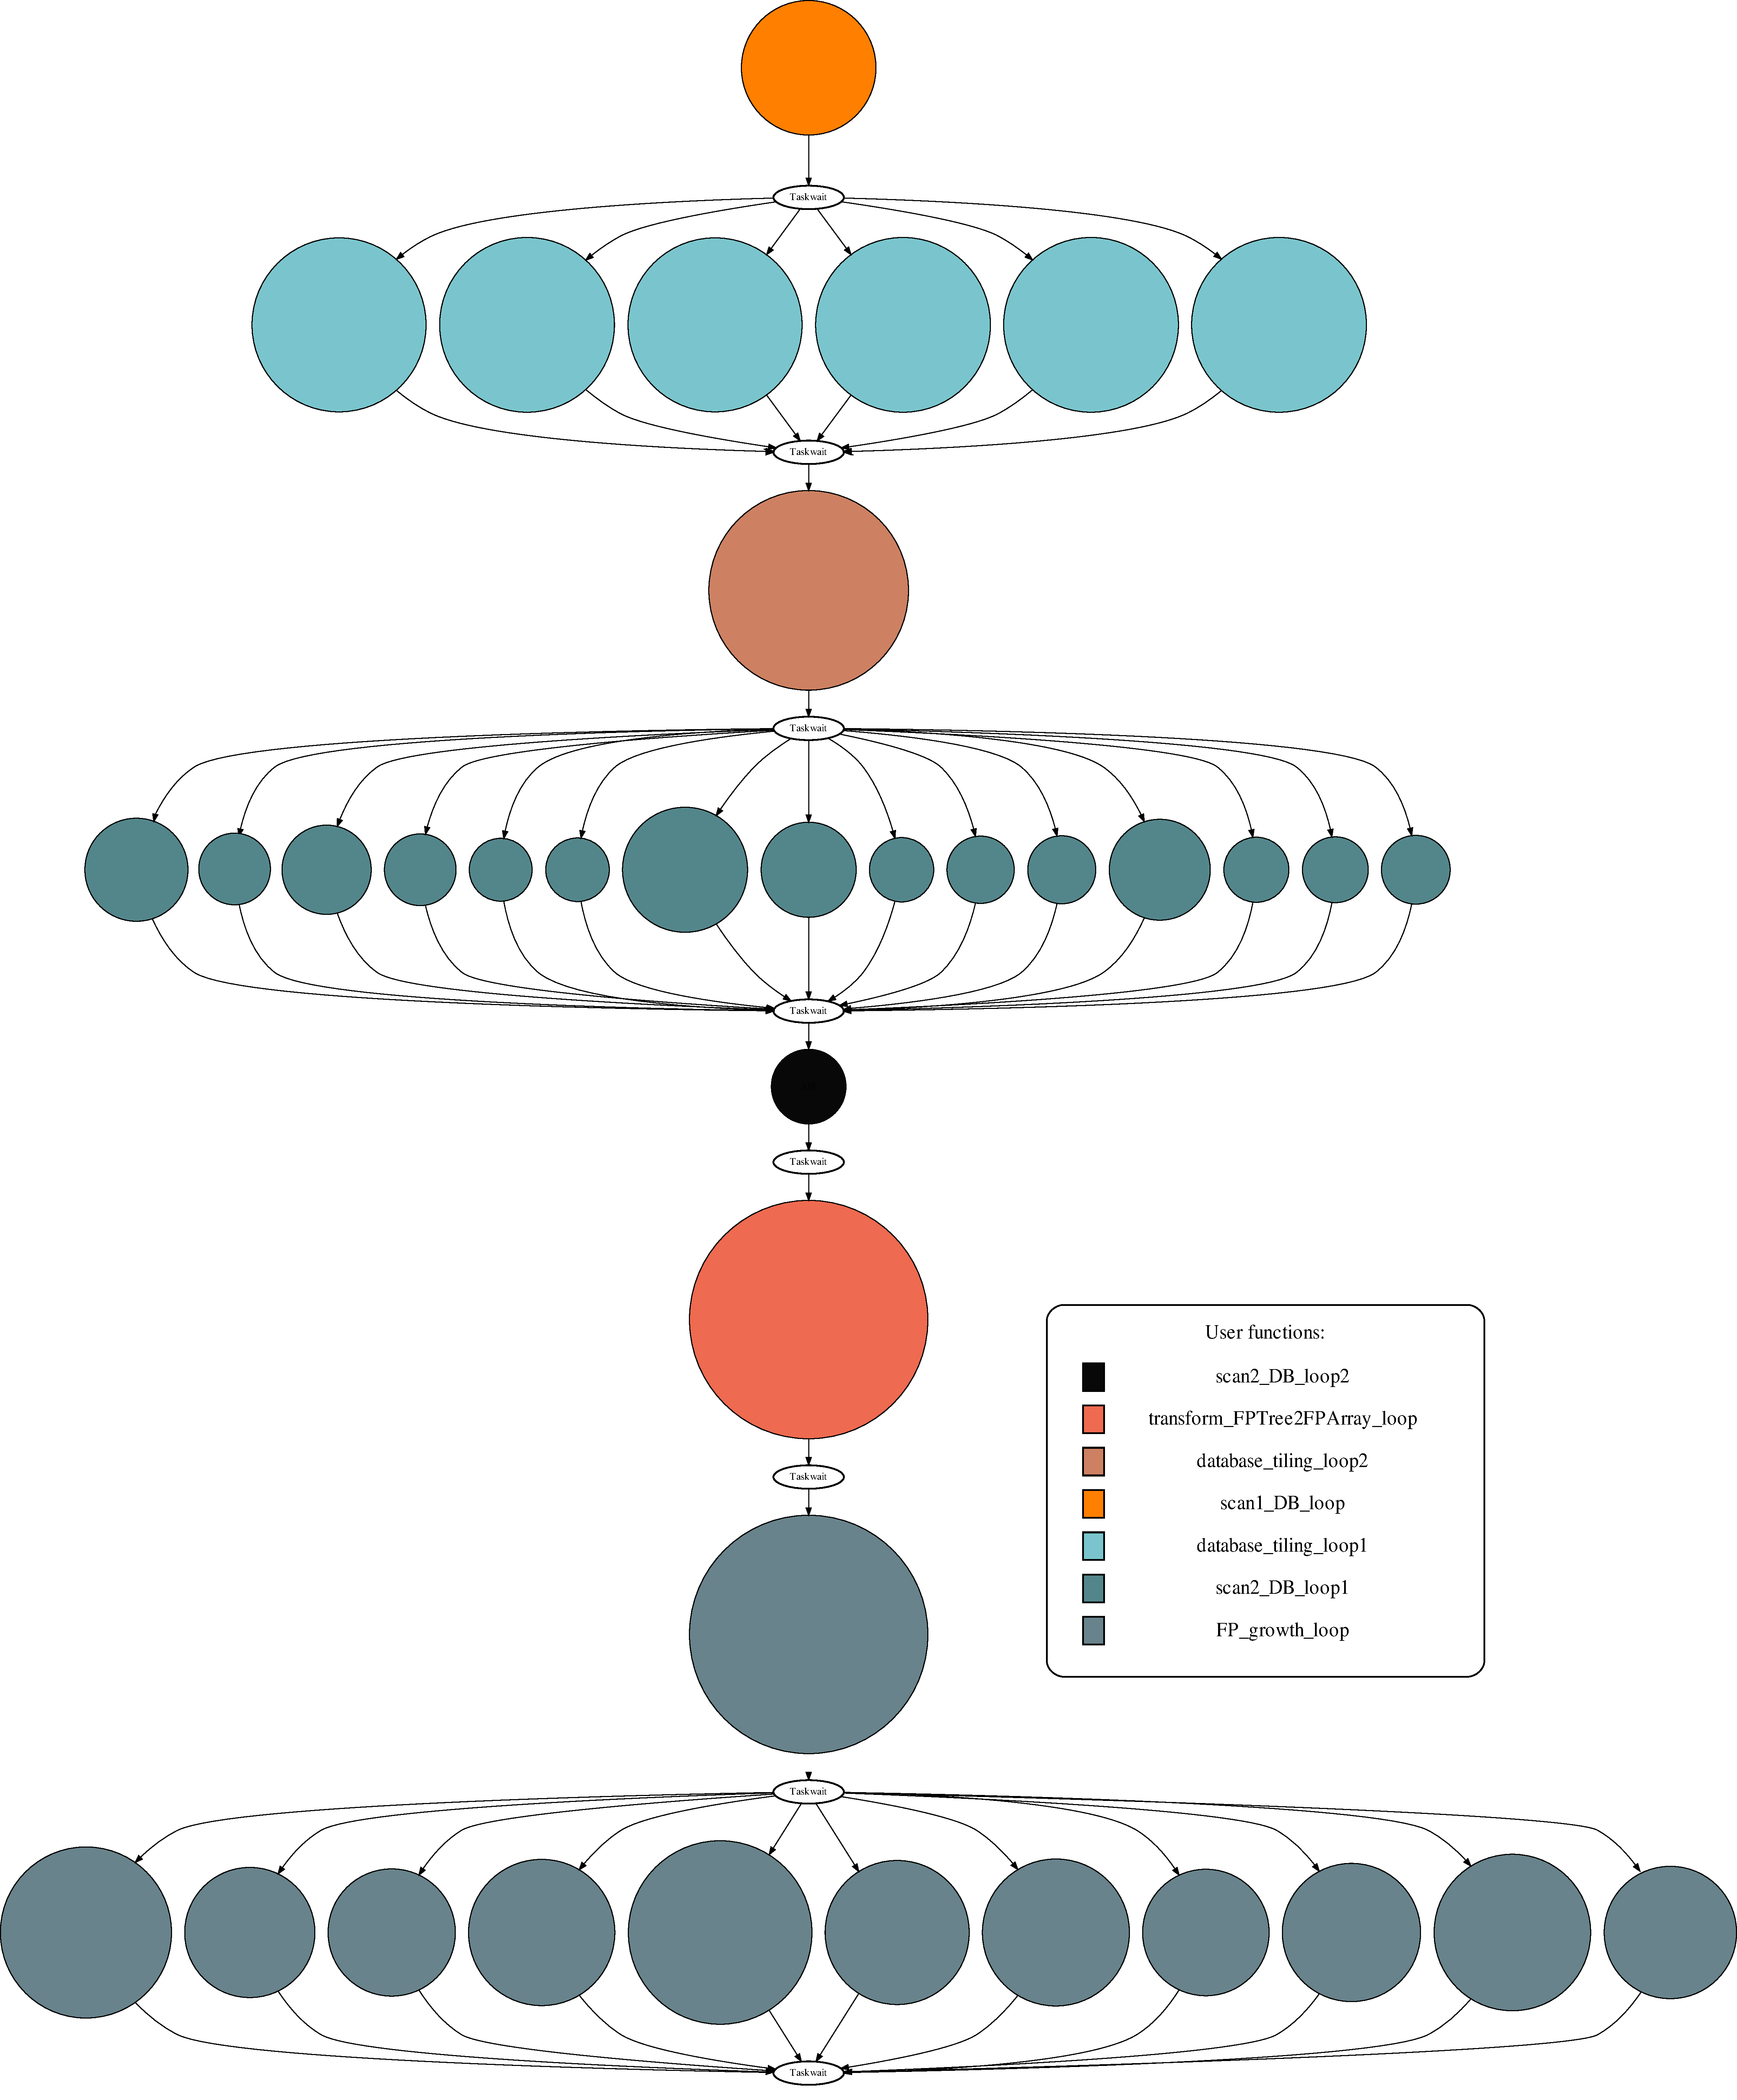
\includegraphics[width=.8\columnwidth]{ifcg/figures/freqmine_taskgraph}%
	\caption{Task-graph of freqmine application.  Edges represent data dependencies among
tasks.}
	\label{fig:freqmine_tg}%
	\vspace{.5cm}
\end{figure}

\paragraph{\textbf{Freqmine}}
Data mining application that makes use of an array-based version of the Frequent Pattern
(FP) growth method for Frequent Itemset Mining~\cite{conf/fimi/GrahneZ03}.

\paragraph{\textit{Pthreads}}
The application uses a compact tree data structure, denoted \emph{FP-tree}~\cite{Han:2000:MFP:335191.335372}, to store information about frequent patterns of the transaction database.  The FP-tree is coupled with a header table, which is a list of database items, sorted by decreasing order of occurrences.
The FP-growth algorithm traverses the FP-tree structure recursively, constructing new FP-trees until the complete set of frequent itemsets is generated.
There are three parallel kernels.  The \texttt{Build\_FP-tree\_header\_table} kernel performs a database scan 
and counts the number of occurrences of each item.  The result is the FP-tree header table.   
\texttt{Build\_Prefix\_tree} kernel performs a second database scan required to build the prefix tree
and the \texttt{Data\_Mining} kernel obtains the frequent itemset information by using the previous two structures.  It creates
an additional lookup table, which allows faster traversals on sparse itemsets.
The original \PARSEC{} benchmark uses OpenMP2.0 for loop parallelization inside each kernel.  

\begin{figure}[ht!]%
	\center
	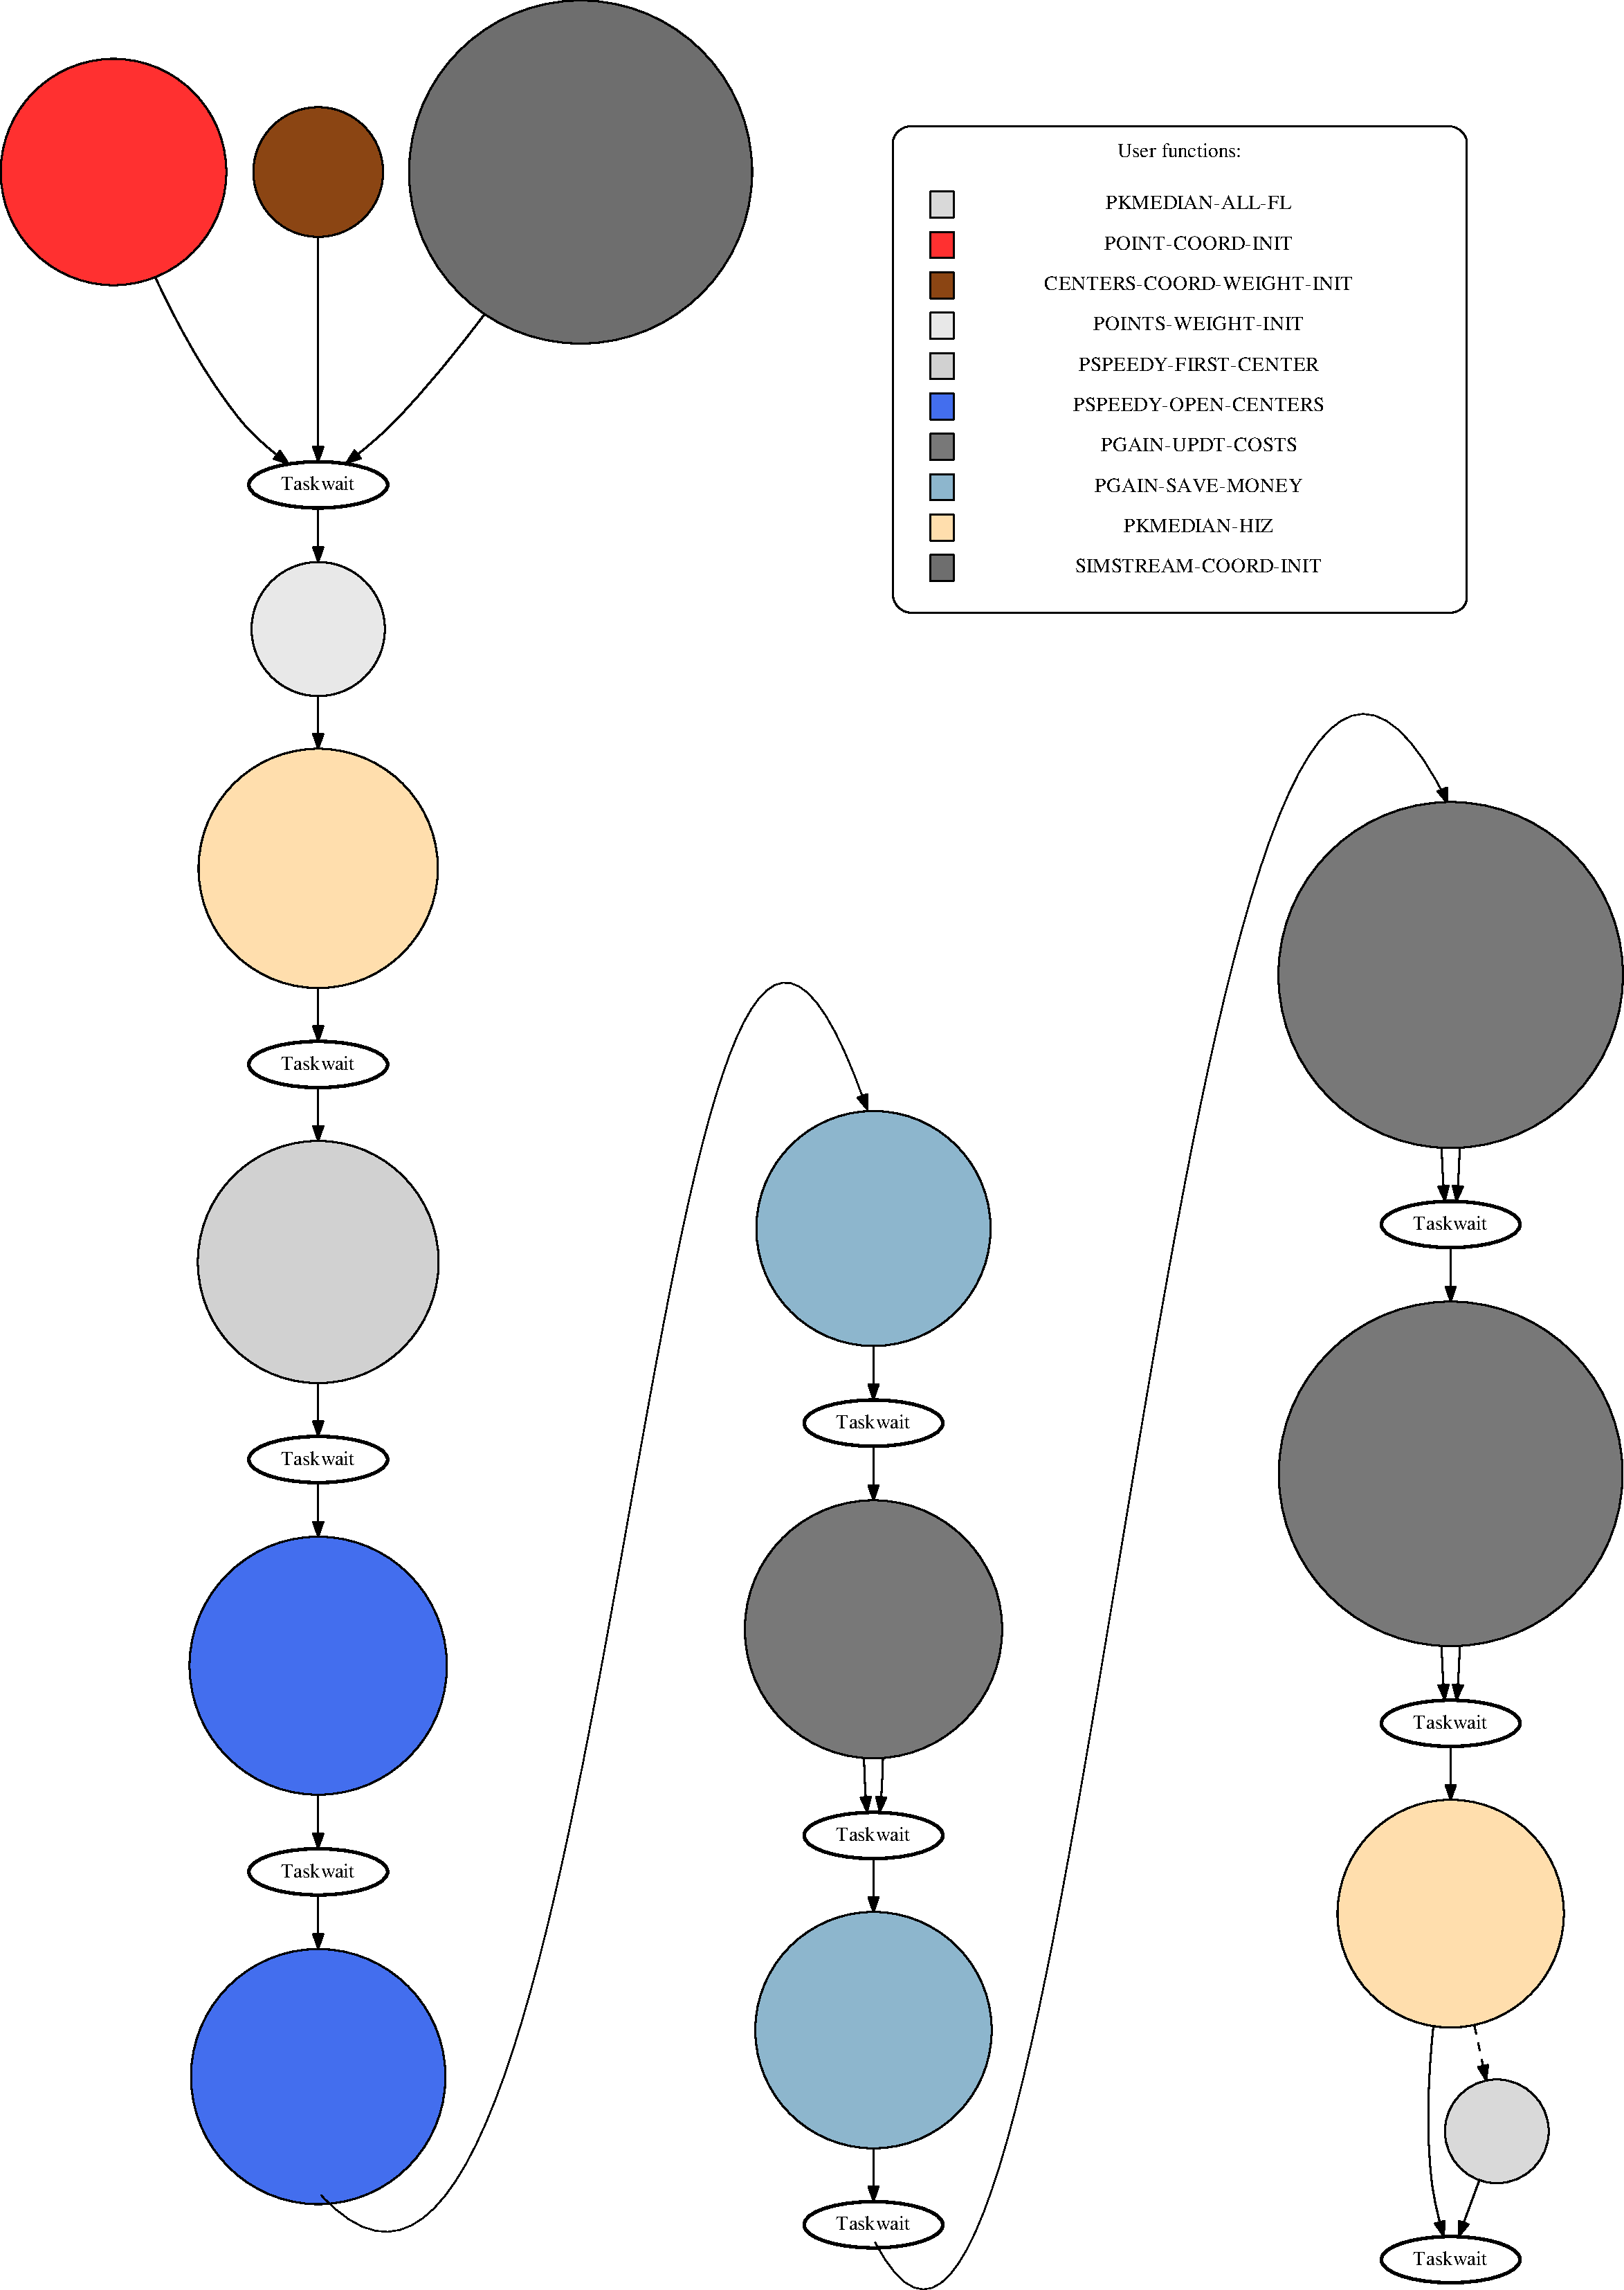
\includegraphics[width=.6\columnwidth]{ifcg/figures/streamcluster_taskgraph}%
	\caption{Task-graph of streamcluster application.  Edges represent data dependencies among
tasks.}
	\label{fig:streamcluster_tg}%
	\vspace{.5cm}
\end{figure}



\paragraph{\textit{Task-based}}
In our implementation we taskify each iteration. We do not use any dataflow relations in this application, and resolve to 
adopt the locking and barrier synchronization used in the original OpenMP version.
The barrier synchronization is shown in the task graph in figure \ref{fig:freqmine_tg}.

\paragraph{\textbf{Streamcluster}}
Streamcluster is a kernel that solves the online clustering problem. 
It takes a stream of points and then groups them in a predetermined number of clusters with their respective centers.  


\paragraph{\textit{Pthreads}}
Up to 90\% of total execution time is spent in function \texttt{pgain}, 
computing whether opening a new center is advantageous or not.  For every 
new point, function \texttt{pgain} calculates the cost of making it a new center by reassigning some points to it and 
comparing it to the minimum distance $d(x,y) = |{x-y}|^2$ between all points $x$ and $y$.
The result is accepted if found to favor the new center.  Data points are statically partitioned by a given block 
size, which determines the level of parallelism in the application. In the Pthreads version this is equal to the number of
threads. 

\paragraph{\textit{Task-based}}
In our implementation we follow a different decomposition strategy, making the number of tasks independent
of the number of partitions.   
Barriers are employed to synchronize accesses
to a partition in both Pthreads and the task-based implementation. 
In the case of Pthreads, an additional user 
implemented library is used for the barriers. 
This library is not required in the case of the OmpSs implementation, as 
the runtime already has a generic barrier implementation.
A task graph of our task-based implementation and the dependencies among tasks is shown in figure \ref{fig:streamcluster_tg}

\paragraph{\textbf{Swaptions}}
Economics application that uses the Heath-Jarrow-Morton (HJM)\cite{RePEc:ecm:emetrp:v:60:y:1992:i:1:p:77-105} for pricing of a portfolio of swaptions. To calculate prices it employs the Monte Carlo simulation.

\begin{figure}[ht!]%
	\center
	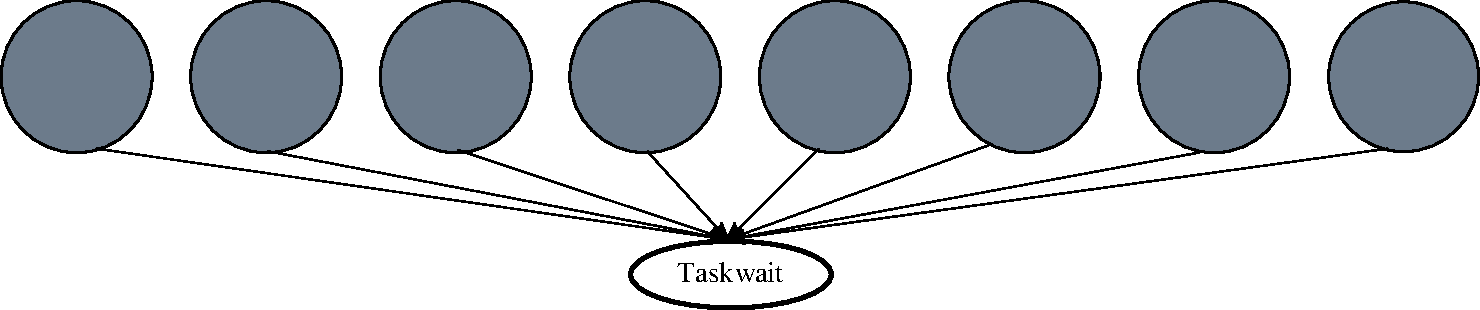
\includegraphics[width=.8\columnwidth]{ifcg/figures/swaptions_taskgraph}%
	\caption{Task-graph of swaptions application.}
	\label{fig:swaptions_tg}%
	\vspace{.5cm}
\end{figure}


\paragraph{\textit{Pthreads}}
The application stores the portfolio into an array. In the Pthreads version, this array is divided by the number of available threads, each thread working on its own part of the array. 

\paragraph{\textit{Task-based}}
We use the exact same strategy, where each task works on a part of the array.  No data dependencies exist between the tasks.
Figure \ref{fig:swaptions_tg} shows the corresponding task graph for the swaptions application.  No dependencies exist between tasks,
synchronization is only achieved through barriers.
%\paragraph{\textbf{x264}}
%An AVC (Advanced Video Coding) video encoder, based on the ITU-T H.264 standard~\cite{H.2642007}.
%It improves over previous video encoding standards at the expense of significantly increased 
%encoding and decoding time.


%The parallel version of x264 extracts parallelism by processing different frames concurrenlty. Initially frames are split in smaller 
%macroblocks of 16x16 pixels.  These macroblocks are processed by a pipeline with a number of stages equal to the number of frames.
%The stages are: \texttt{Read\_frame}, which reads input frames, \texttt{Analyse\_frame}, which creates data dependencies among macroblocks,
%\texttt{Encode\_frame}, which is the encoding state and \texttt{Write\_frame} which writes the encoded frames to the output file.


%The task-based implementation does not use the macroblocks. Instead
%it works on whole frames.  We use two different task types, each spawned for each frame.  The first reads the frame and the second performs the
%three other pipeline stages.  The pipeline stages are synchronized using shared variables. 
 

\section{Programmability}
Different models and languages offer diverse ways to express concepts, such as parallelism or asynchrony.
In this section we evaluate how successful and easy it is to express parallelism using task-based models.  
A good proxy to evaluate how complex a particular implementation is the number of lines of code it takes.
Despite being a metric proposed some decades ago, comparing different programming models in terms of the total number of code lines
is still a valid metric. Indeed, recent publications make an extensive use of it~\cite{Vandierendonck:2011:PPG:2001252.2001265,Dongarra20081}.

%\subsection{Expressiveness}
%\edit{In the Parsec suite we encounter a diverse
%set of parallelization strategies, which however can be grouped into data-parallelism, pipeline parallelism and hybrid between data and pipeline
%parallelism (e.g. \texttt{facesim}).  We were able to express at least the same amount of parallelism in all the 10 benchmarks we used for this study,
%compared to the Pthreads and OpenMP versions.  Additionally, in the cases of \texttt{bodytrack} and \texttt{facesim} we were able to express additional
%parallelism with the use of dataflow annotations and tasks.  Note that in the case of \texttt{dedup}, we adopted a parallelization method with less available
%parallelism than in the case of Pthreads.  We were also able to implement the original Pthreads \texttt{dedup} version but for performance reasons we adopted
%the version with less parallelism.   Section~\ref{sec:implementation} explains this decision in detail.}


%\edit{Although we were able to implement 10 out of the 10 benchmarks, it is possible that we could obtain better results and express additional parallelism in some
%cases, but not with the current standard syntax that OpenMP 4.0 offers.  As discussed in Section \ref{sec:implementation}, the current syntax could benefit from
%extensions that could express data dependencies among irregular and dynamic data structures.  The current OpenMP 4.0 standard is focused on continuous data structures.}

\begin{figure*}[!htbp]
        \centering
        \begin{subfigure}[b]{0.8\textwidth}
                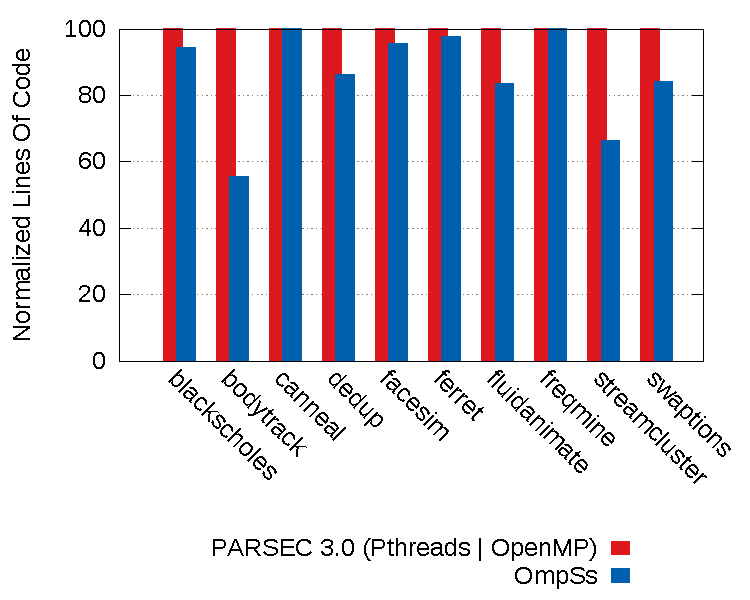
\includegraphics[width=\textwidth]{ifcg/figures/absolute_loc_norm}%
                \caption{Comparison between all source files.}%
                \label{fig:absolute_loc}
                \vspace{0.4cm}
        \end{subfigure}%
				\hfill
        \begin{subfigure}[b]{0.8\textwidth}
        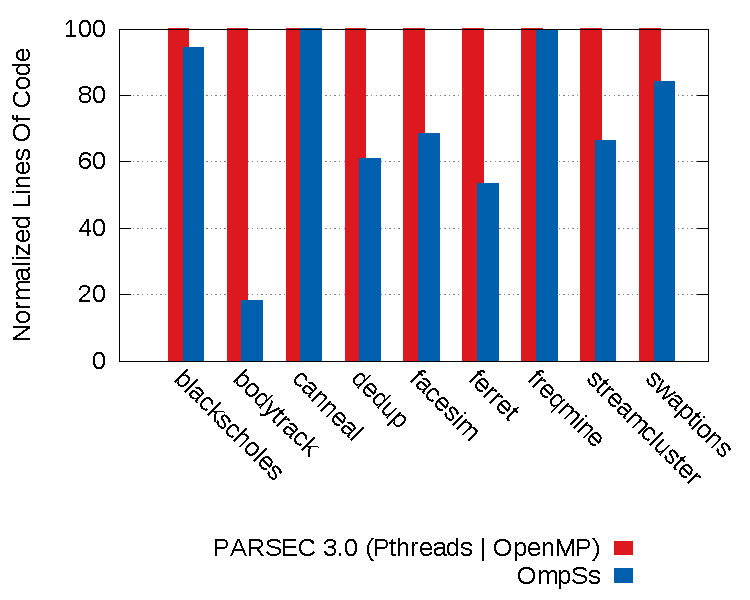
\includegraphics[width=\textwidth]{ifcg/figures/relative_loc_norm}%
        \caption{Comparison between only source files containing parallel code.}%
        \label{fig:relative_loc}%
        \end{subfigure}%
  \caption{Comparison of lines of code between our task-based implementations and the original Pthreads or OpenMP versions.}
        \label{fig:loc_comparison}
\end{figure*}


\subsection{Lines Of Code}
\label{sec:lines}
The reduction of the lines of code (LOC) attests to a more compact and readable code.
%keeping in mind that the actual 
%algorithm complexity remains unchanged.}
In some of our PARSEC task-based implementations, a simple pragma directive replaced application 
specific schedulers, scheduling queues, thread pooling mechanisms and lock synchronization.
We do not change the algorithm in any of the task-based parallel strategy implemented in the PARSEC suite.
Figure~\ref{fig:absolute_loc} shows a normalized comparison between the lines of code of our task-based implementations and the original Pthreads/OpenMP implementations of the PARSEC 3.0 distribution.
The PARSEC 3.0 versions we refer to are always the Pthreads versions, except in the case of \texttt{freqmine} where, since there is no Pthread version available, the OpenMP2.0 version is taken as reference.
We preprocess all source files so that they only contain lines of code relevant to the respective programming model\footnote{PARSEC benchmarks contain mixed serial, Pthreads, OpenMP and TBB source code, and make use of macros to enable conditional compilation for only one programming model at a time.}.
%The LOC column in Table~\ref{tab:parsec} shows the total lines of code for each application, counting all source files.
%Upon careful inspection we can observe that the task-based version requires less lines of code, however parallel code is only a fragment of the sources
%for most applications.  
Figure \ref{fig:relative_loc} shows the total lines of code comparison when we only consider files that are relevant to the parallel 
implementation, that is, files that contain calls to Pthreads or task invocations, asynchronous I/O implementations, atomic primitives, etc.
In this graph we see that the reductions in terms of lines of code of our task-based strategies are significant.
In case of \texttt{bodytrack}, we are able to remove 81\% of the code lines. Since \texttt{Bodytrack} implements its own scheduler to deal with load balancing, there is much room for code reductions by replacing this ad-hoc mechanisms for a few pragma annotations.

By using tasks and dataflow relations, it is very easy to implement pipelines.  We adopt this approach for both \texttt{dedup} and \texttt{ferret}, 
which result in a significant decrease in LOC (38\% and 46\%, respectively). Figure~\ref{lst:ferret-ompss} shows the pipeline code for \texttt{ferret}.  All that is required is
to taskify the different pipeline stages and make sure that dataflow relations force in-order execution of tasks in the same pipeline instance. The Pthreads version requires the implementation
 of queues between each stage, which must also be safe to use by multiple threads and concurrent accesses.
\texttt{Streamcluster} and \texttt{fluidanimate} task-based versions also reduce lines of code by 33\% and 21\% respectively, by removing the need for an additional, user implemented, barrier library. 
\texttt{Blackscholes} and \texttt{swaptions} are relatively simple applications, containing only one do-all parallel loop each.
In these cases the LOC difference is minimal (0.5\% and 15\%, respectively). 
In the cases of \texttt{canneal} and \texttt{freqmine} we see no difference in LOC. 
\texttt{Canneal} is not a data parallel application and in both cases Pthreads and tasks are used merely as thread launching mechanism, while the synchronization effort is essentially the same. 

It is worth noting that conventional synchronization primitives can still be used with tasks, without penalizing the programmer.
\texttt{Freqmine} is implemented in OpenMP, which excels at parallelizing loops with very little effort from the programmer and is the ideal programming model for this application. 
In our implementation we simply taskify the loops, essentially not affecting LOC.
\texttt{Facesim} also benefits from the tasks-based approach by 37\%, as the queues required to schedule work have been 
completely removed. 
Overall, we see that the task-based model reduces code size and by \AVERAGELOC{} on average.



\begin{figure}[p]
        \centering
        \begin{subfigure}{0.8\textwidth}
                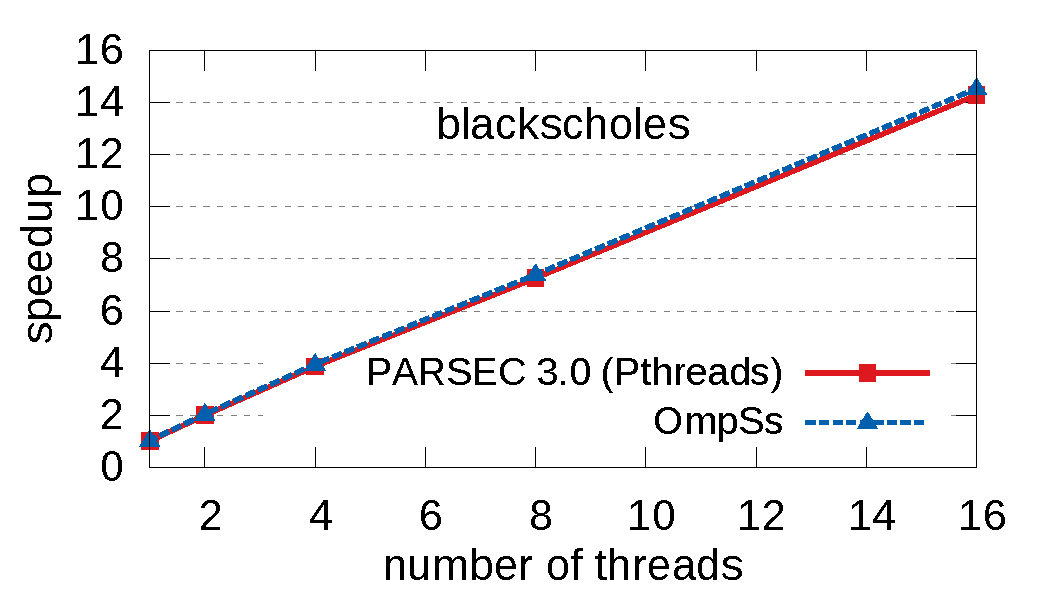
\includegraphics[width=\textwidth]{ifcg/figures/blackscholes_scale}
                \label{fig:blackscholes_scale}
        \end{subfigure}%
\hfill
        \begin{subfigure}{0.8\textwidth}
                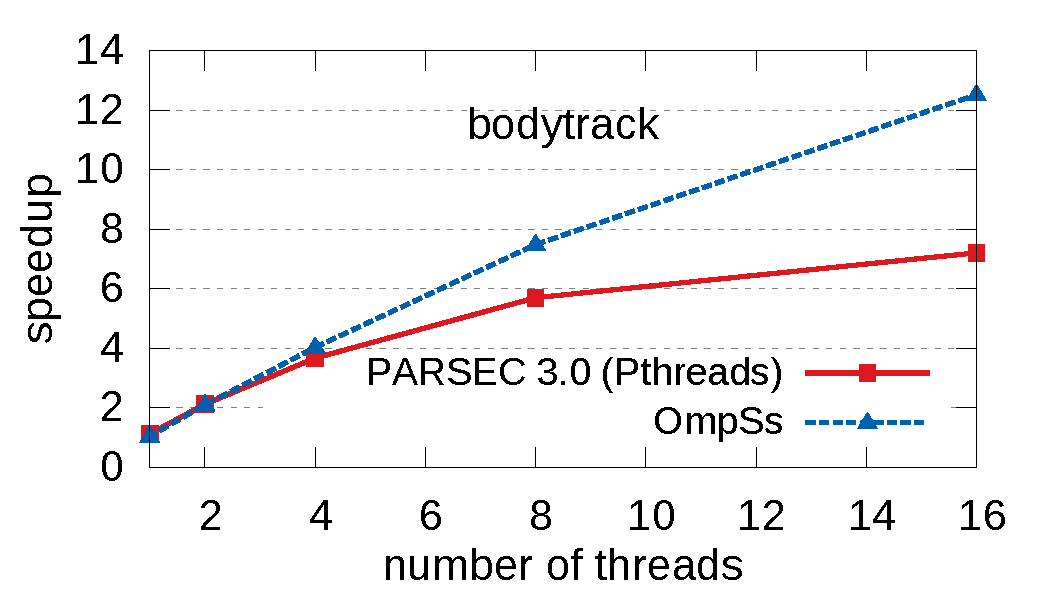
\includegraphics[width=\textwidth]{ifcg/figures/bodytrack_scale}
                \label{fig:bodytrack_scale}
        \end{subfigure}
        
				\begin{subfigure}[b]{0.8\textwidth}
                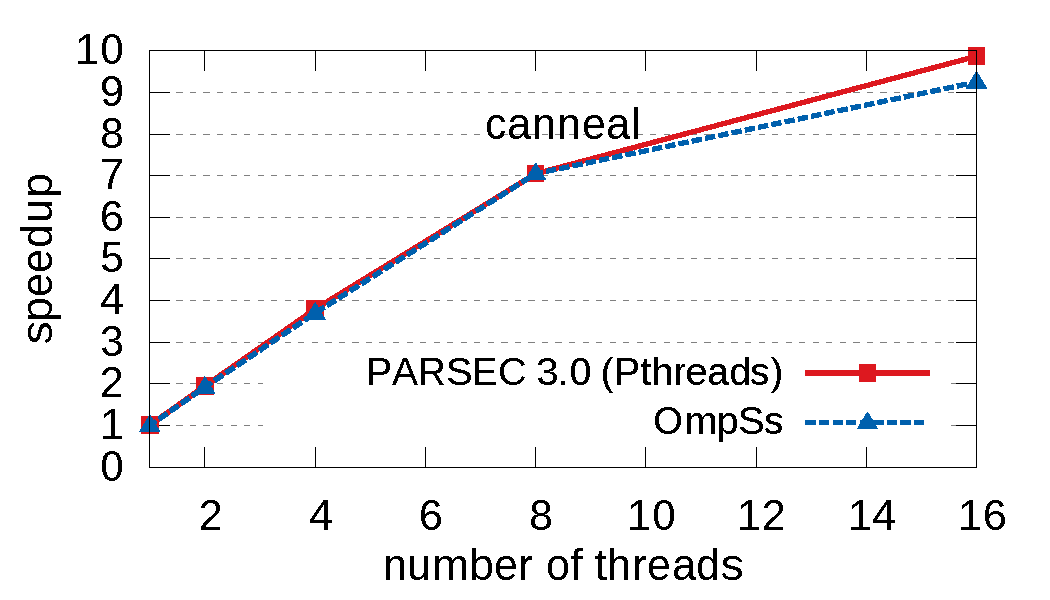
\includegraphics[width=\textwidth]{ifcg/figures/canneal_scale}
                \label{fig:canneal_scale}
        \end{subfigure}
      \caption{Comparison of scalability between the task-based implementations and the original (Pthreads/OpenMP) versions.}
			\label{fig:scalability_graphs_1}
\end{figure}

\begin{figure}[p]
				\centering
        \begin{subfigure}[b]{0.8\textwidth}
                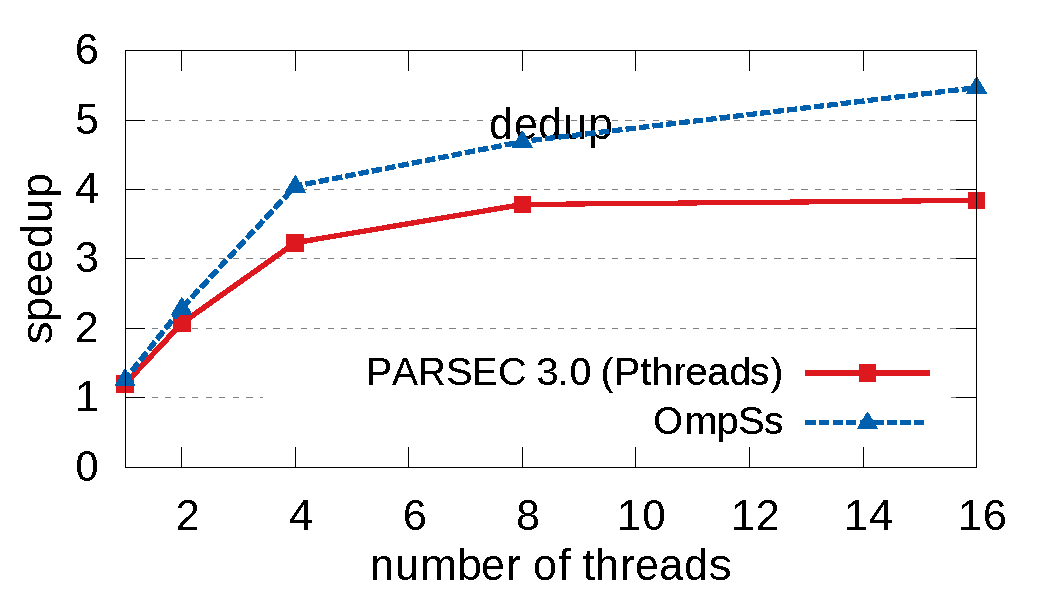
\includegraphics[width=\textwidth]{ifcg/figures/dedup_scale}
                \label{fig:dedup_scale}
        \end{subfigure}
\hfill
        \begin{subfigure}[b]{0.8\textwidth}
                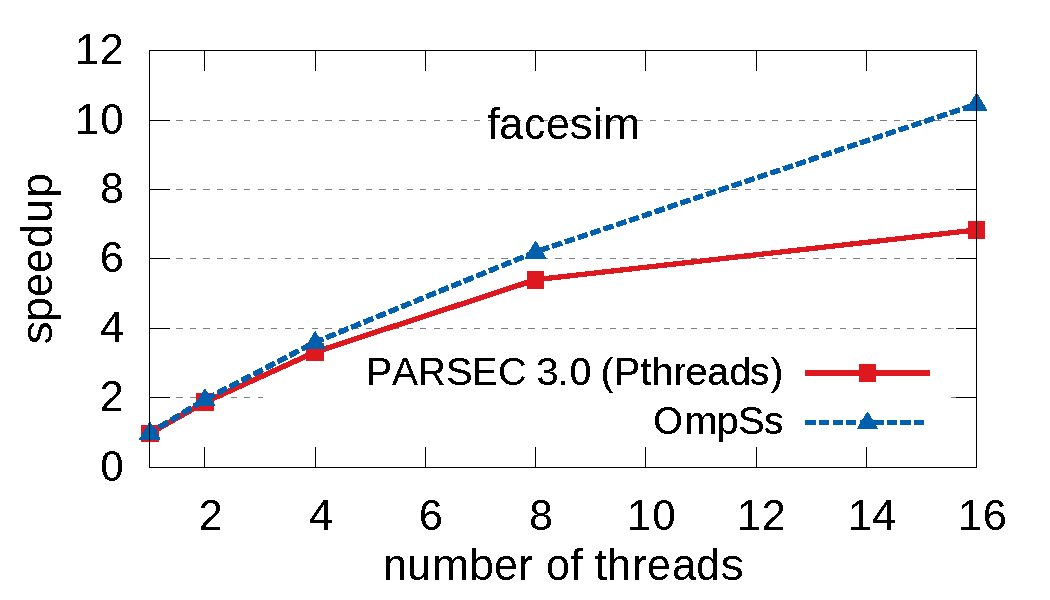
\includegraphics[width=\textwidth]{ifcg/figures/facesim_scale}
                \label{fig:facesim_scale}
        \end{subfigure}
\hfill
				\begin{subfigure}[b]{0.8\textwidth}
                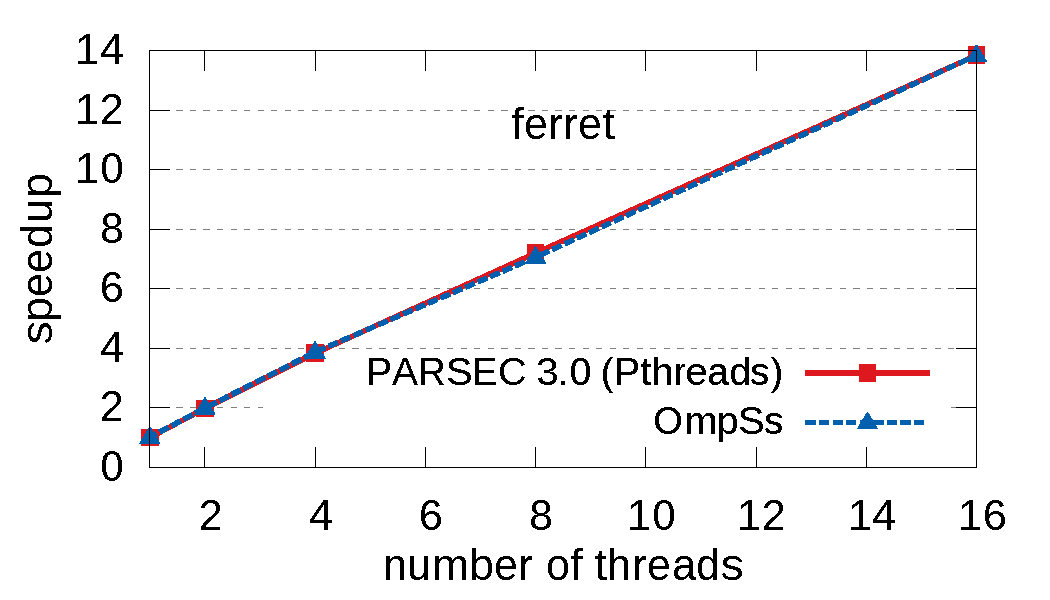
\includegraphics[width=\textwidth]{ifcg/figures/ferret_scale}
                \label{fig:ferret_scale}
        \end{subfigure}%
      \caption{Comparison of scalability between the task-based implementations and the original (Pthreads/OpenMP) versions.}
			\label{fig:scalability_graphs_2}
\end{figure}

\begin{figure}[p]
				\centering
				\begin{subfigure}[b]{0.8\textwidth}
                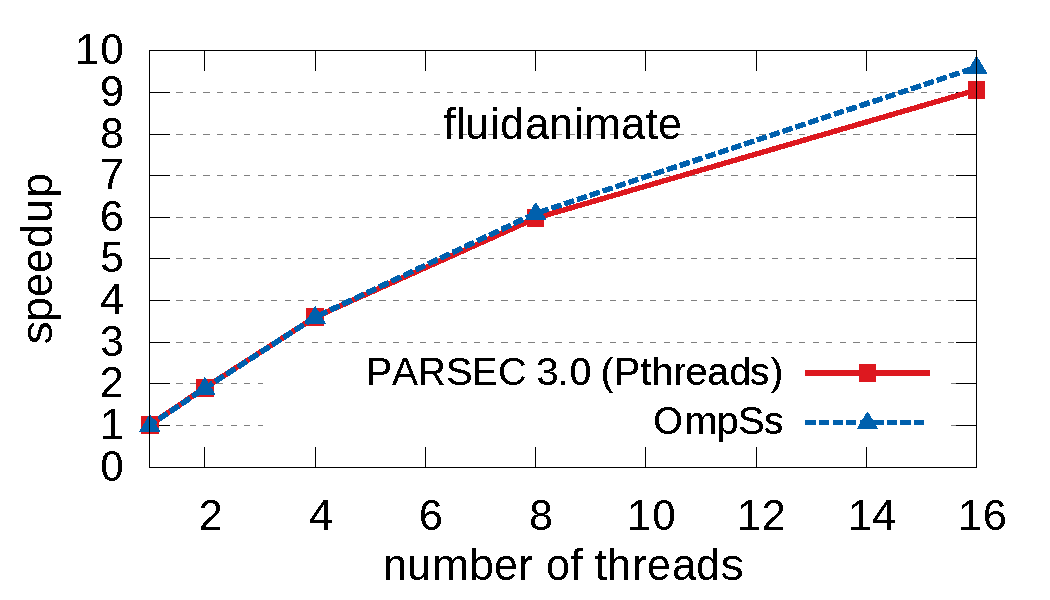
\includegraphics[width=\textwidth]{ifcg/figures/fluidanimate_scale}
                \label{fig:fluidanimate_scale}
        \end{subfigure}
\hfill
        \begin{subfigure}[b]{0.8\textwidth}
                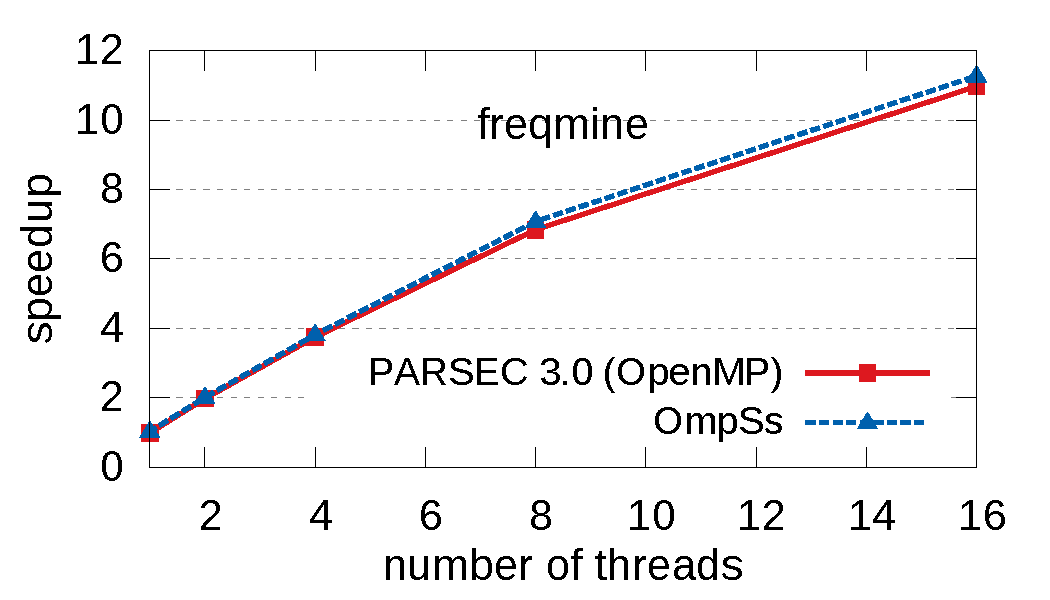
\includegraphics[width=\textwidth]{ifcg/figures/freqmine_scale}
                \label{fig:freqmine_scale}
        \end{subfigure}
\hfill        
				\begin{subfigure}[b]{0.8\textwidth}
                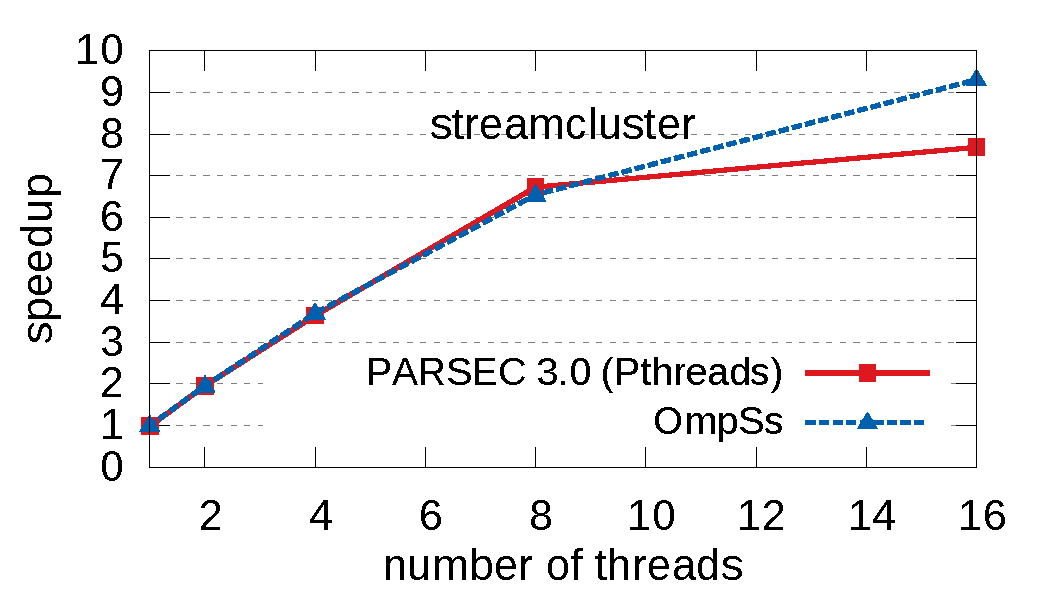
\includegraphics[width=\textwidth]{ifcg/figures/streamcluster_scale}
                \label{fig:streamcluster_scale}
        \end{subfigure}
			\caption{Comparison of scalability between the task-based implementations and the original (Pthreads/OpenMP) versions.}
			\label{fig:scalability_graphs_3}
\end{figure}

\begin{figure}[ht]
				\centering
        \begin{subfigure}[b]{0.8\textwidth}
                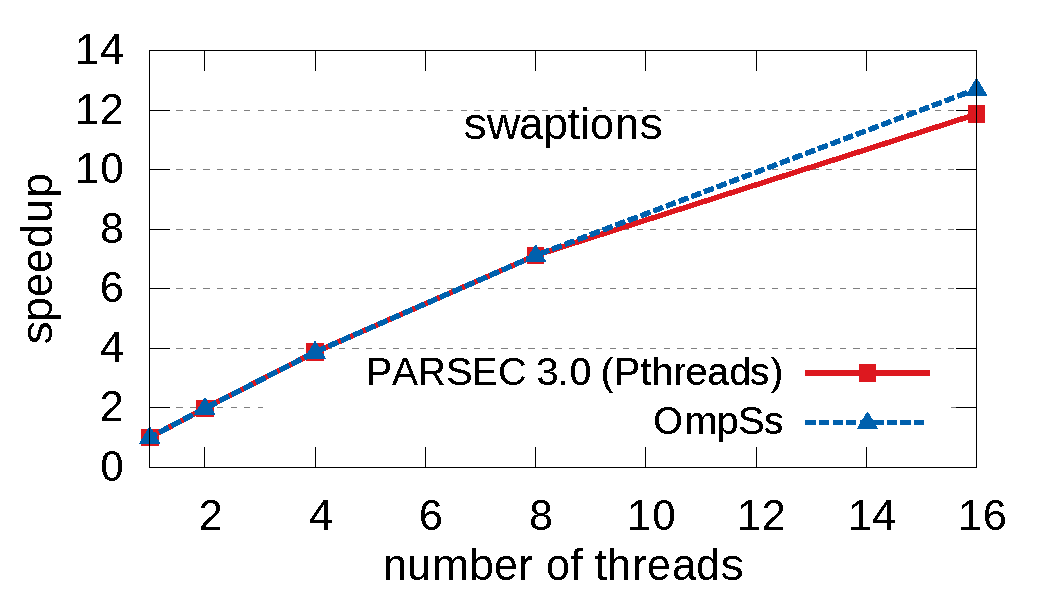
\includegraphics[width=\textwidth]{ifcg/figures/swaptions_scale}
                \label{fig:swaptions_scale}
        \end{subfigure}
      \caption{Comparison of scalability between the task-based implementations and the original (Pthreads/OpenMP) versions.}
			\label{fig:scalability_graphs_4}
			\vspace{.5cm}
\end{figure}





\section{Performance}
\label{sec:task_bench_evaluation}

%Performance is a significant factor when evaluating a parallel programming model.  
In this section we compare our task-based implementations to the original \PARSEC{} implementations in Pthreads or OpenMP.

\subsection{Scalability}
\label{subsec:scalability}
Figures~\ref{fig:scalability_graphs_1},\ref{fig:scalability_graphs_2},\ref{fig:scalability_graphs_3},\ref{fig:scalability_graphs_4} 
shows how the task-based codes scale compared to the \PARSEC{} Pthread/OpenMP versions. 
Results are shown individually per benchmark as we increase the number 
of cores assigned to the application and normalized to the execution time of the serial implementation
\footnote{The PARSEC benchmark suite provides a serial implementation for \texttt{blackscholes}, \texttt{bodytrack}, \texttt{dedup}, \texttt{ferret}, 
\texttt{freqmine} and \texttt{swaptions}. 
For the other benchmarks, the original Pthreads parallel implementation executed on a single core is considered as the baseline.}
 of the application. Nearly all applications scale linearly up to 4 cores.
%However, with 8 and 16 cores, 
%performance improvements diminish.
%reaching 30\%, 42\% and 34\% improvements, respectively.

In the case of \texttt{bodytrack}, as described in Section~\ref{sec:parsecss_implementation}, by concurrently executing different frames, there is always enough work for all threads, while by taskifying the 
output stage of each frame, we overlap this I/O bottleneck with other computation stages. The speedup when run on 16 cores is 12.1x, while the Pthreads implementation reaches a poor 6.8x speedup when run on 16 cores.
The \texttt{dedup} application has a very expensive stage that writes the compressed data to the output file. 
Our task-based implementation is very effective in overlapping this time with computation from the compression stage. Also, the task-based version does not have to reorder the data chunks, 
since the I/O execution takes place in-order as dictated by dataflow relations. This results in an impressive 30\% performance improvement of the OmpSs version with respect to Pthreads when run on 16 cores.
The Pthreads \texttt{facesim} implementation is burdened by barriers that limit available parallelism. 
By using dataflow relations 
%among 
%the different parallel loops and stages, we remove all barriers, except the barriers before starting and finishing the \texttt{CG} kernel,
%which protect the residual calculation. In Section~\ref{sec:implementation} we discuss two different 
%implementations, one only with tasks and one using also OpenMP equivalent loops. Figure\ref{fig:scalability_graphs} shows the speedup for the later version.
%Our initial implementation gave 8.7\% performance improvement compared to the Pthreads version. 
%The issue with our initial approach was that
%some tasks had very high task creation overhead, which led to unfavorable scheduling and load imbalance among threads. 
%We identified some opportunities 
%to overlap computation with task creation, hiding any runtime overheads, but this did not eliminate them completely. By using the loop construct 
%we managed to minimize the task creation overhead. 
we taskify sequential segments of significant cost we effectively
synchronize them with parallel sections preceding and following it.
The performance improvements comes from the overlap of sequential computations with parallel sections.
The task-based parallelization of \texttt{facesim} reaches a speedup of 10.2x when run on 16 cores, while the PARSEC code only reaches a 6.4x speedup.

In the cases of \texttt{blackscholes}, \texttt{canneal}, \texttt{ferret}, \texttt{fluidanimate}, \texttt{freqmine} and \texttt{swaptions}, the Pthreads/OpenMP
versions already achieve good scalability results. With the exception of \texttt{ferret}, the task-based codes have very close resemblance to their Pthreads/OpenMP counterparts, and have offered reduced 
opportunities for \OMPSS{} to dynamically exploit additional parallelism.  
The parallel implementation in these applications, with the exception of \texttt{ferret}, is limited to parallel do-all loops with 
barrier synchronization, essentially exploiting the same amount of parallelism among all versions (OmpSs/Pthreads/OpenMP). 

In the case of \texttt{ferret}, although the code is substantially different, both versions employ the same pipeline model and deliver the same level of parallelism, which is already  high in the Pthread version.  
We express 
a bit of extra parallelism by extending the pipeline with multiple stages, which write to the output file, effectively overlapping some communication with computation. 
However, the final impact in the 
total execution time is limited as the time needed to write the output file is a very small fraction of the total execution time. 
Finally, we observe performance gain (18\%) in \texttt{streamcluster}, which can be partly attributed to the more efficient 
barrier implementation of \OMPSS{}, when compared to the user implemented barriers of the Pthreads version. 
However, the most important performance drawback 
that the original Pthreads implementation suffers from, is the negative NUMA effects.
This issue is observed when we run our experiments on a two socket system.
The Pthreads code partitions the working set by the number of available cores.
We employ a different partition scheme to counter the 
NUMA effects. Through experimentation we observe that the best results can be obtained when using 80 blocks. 

%However, when we use the 
%same number of partitions as the Pthreads version, which is 16, we obtain a moderate speedup of 9\%.  We can observe how the 
%same results in figure~\ref{fig:granularity_comparison}.  Green bar represents the task-based version 
%that uses the same granularity as Pthreads, while the blue bar shows the performance of \texttt{streamcluster}, when using 80 blocks.

\begin{figure}[t]
  \centering
  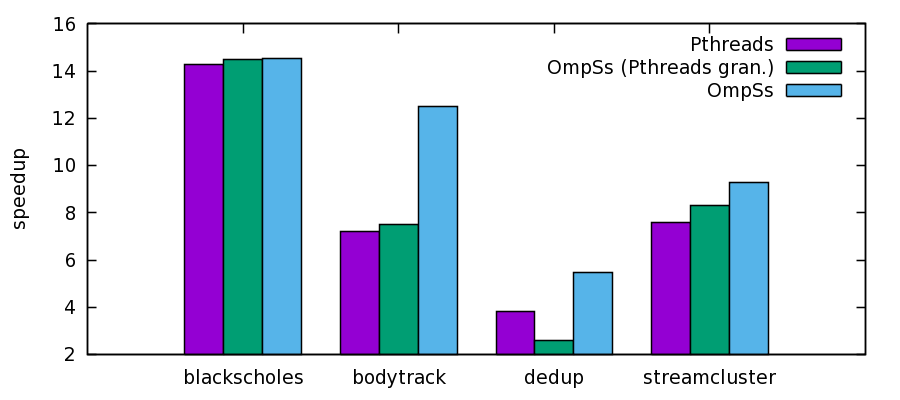
\includegraphics[width=.9\textwidth]{ifcg/figures/parsec_comparison}
  \caption{Speedup comparison for Pthreads and OmpSs with the same granularity, as well as our optimized OmpSs version, when run on 16 cores. Results are normalized to the sequential version of the original code.}
  \label{fig:granularity_comparison}
	\vspace{0.5cm}
\end{figure}

\subsection{Task Granularity Impact}
The granularity of individual tasks is an important factor that needs to be considered when parallelizing an application.
Small task granularity can reduce load imbalance  
but such performance benefits can be neglected by the overhead of the runtime system, as it has to create and schedule more tasks.
Results in Section~\ref{subsec:scalability} show how tuning the task granularity brings performance benefits in some cases (\texttt{blackscholes}, \texttt{bodytrack}, \texttt{dedup} and \texttt{streamcluster})
while in others it is better to keep the same parallel granularity as the \PARSEC{} distribution codes (\texttt{canneal}, \texttt{facesim}, \texttt{ferret}, \texttt{freqmine} and \texttt{swaptions}).
 
In order to provide a more comprehensive comparison, this section examines the performance 
of \texttt{blackscholes}, \texttt{bodytrack}, \texttt{dedup} and \texttt{streamcluster} when using exactly the same granularity as in the \PARSEC{} distribution code.
Figure~\ref{fig:granularity_comparison} shows the speedup of these benchmarks when run on 16 cores. 
The purple bar shows the speedup of the Pthreads version, the green one shows the speedup of a task-based implementation that has the same parallel granularity as its Pthreads counterpart.
Finally, the light blue bar shows the speedup of the optimal task-based implementations discussed in Sections~\ref{sec:parsecss_implementation} and~\ref{subsec:scalability}. 

For the cases of \texttt{blackscholes} and \texttt{streamcluster} the parallelization scheme followed in the three codes (Pthreads and the two OmpSs versions) is the same. 
The difference between the two OmpSs versions is the granularity of the block sizes that are processed per task.
In case of \texttt{blackscholes}, the OmpSs implementation with the same granularity as Pthreads does not perform better since the parallelism of this benchmark follows a fork-join model.
In the case of \texttt{streamcluster}, the task-based implementations always improve the Pthreads performance, even if they operate following the same parallelization scheme and granularity as the Pthreads version.
These improvements come from the NUMA effects correction that the OmpSs versions carry out.

In the case of \texttt{bodytrack} the optimal OmpSs implementation follows a quite different parallelization scheme than the original Pthreads code, as explained in Section~\ref{sec:parsecss_implementation}. 
We consider a trivial implementation in OmpSs where we follow the same parallelization strategy as in Pthreads. 
As shown in Figure~\ref{fig:granularity_comparison}, we do not observe any significant difference in performance among Pthreads and the equivalent OmpSs implementation. 
However, the new parallelization scheme is not applicable to Pthreads as it requires to synchronize the workload by explicit dependencies, which are not available in the Pthreads API.

In the case of \texttt{Dedup}, the trivial Pthreads-like implementation performs poorly, achieving a speedup of 2.6x. 
In this implementation, each pipeline stage is taskified following the Pthreads approach. 
Each large chunk is partitioned into smaller chunks, that will spawn three new tasks (\texttt{Compress}, \texttt{Deduplicate}
and \texttt{WriteOutput}). 
This level of granularity creates hundreds of thousands of tasks, increasing the runtime's overhead significantly. 
In contrast, the optimized task-based version operates at the granularity of the large chunks, creating only a few hundreds of tasks, effectively reducing the runtime overhead. 
%The number of tasks is not the only factor that can influence performance, as their duration is also important. In the fine grain task-based version, some tasks take a very short time to execute. 
%For example \texttt{Deduplication} tasks simply try to insert a single new chunk in a hashtable.

%In general, when following the exact same parallelization strategy and task granularity, Pthreads and OmpSs obtain very similar performance. However, the number of tasks and their size can negatively impact the overall performance. Consequently, users should avoid flooding the runtime system with tasks that run for very short time. Finally, the asynchronous nature of task-based programming models and their programmability allows the users to tune the parallelization strategy or implement more advanced techniques that lead to better final performance.
In some cases, OmpSs can over-perform Pthreads even if the same parallelization scheme and granularity is followed, like the \texttt{streamcluster} results demonstrate.
In some other cases (\texttt{dedup} and \texttt{bodytrack}), the performance improvements come from an optimized parallelization scheme.
Such new schemes could be hardly implemented in Pthreads since they require a direct synchronization via explicit dependencies, which is not available in the Pthreads API.
Finally, in case of simple fork-join applications (i. e. \texttt{blackscholes}) our performance benefits just come from further optimizing the parallel granularity.


\begin{figure*}[p]
  \centering
  \begin{subfigure}{0.75\textwidth}
                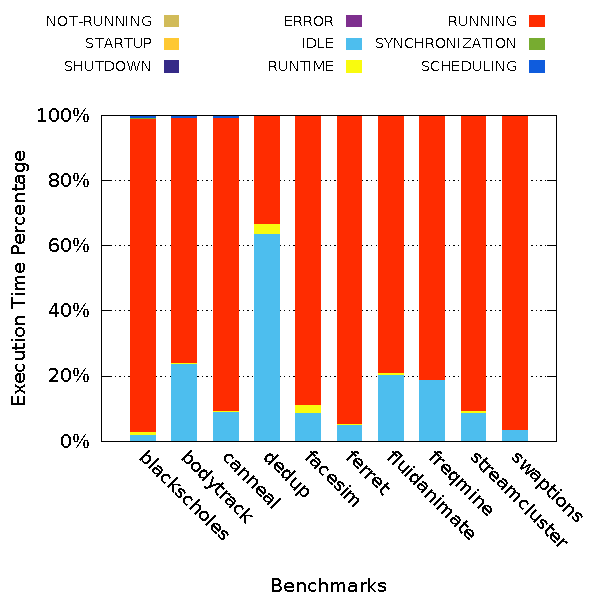
\includegraphics[width=\textwidth]{ifcg/figures/worker-runtime-breakdowns-8}
                \caption{Average time over 8 threads}
                \label{fig:runtime_breakdown_8}
  \end{subfigure}
	\hfill
  \begin{subfigure}{0.75\textwidth}
                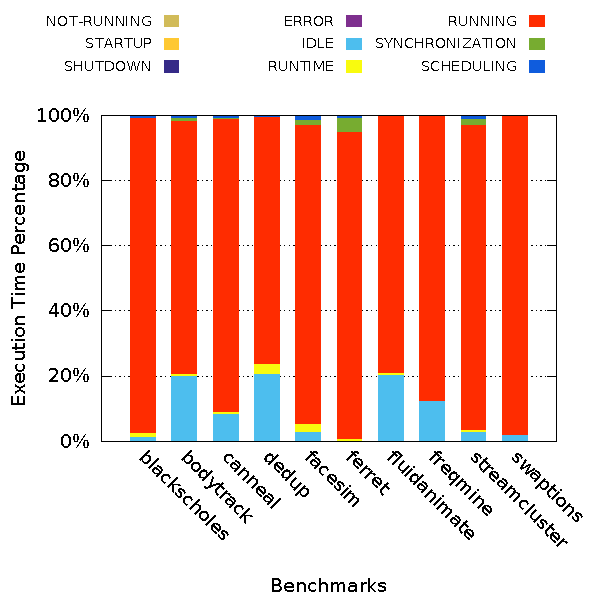
\includegraphics[width=\textwidth]{ifcg/figures/master-runtime-breakdowns-8}
                \caption{Main thread runtime breakdowns}
                \label{fig:master_runtime_breakdown_8}
  \end{subfigure}
        \caption{Runtime breakdowns when running on an 8-core configuration.}
        \label{fig:runtime_breakdown}
	\vspace{.5cm}
\end{figure*}



%\vspace{-0.8cm}
\subsection{Runtime System Overhead}
%\vspace{-0.15cm}
Task creation, scheduling and data dependencies tracking are all handled by the OmpSs runtime system. In this section, we evaluate the impact of these activities over the final parallel performance.
Figure~\ref{fig:runtime_breakdown_8} shows a breakdown of the total execution time of each application. 
Each bar shows the breakdown of one application after averaging the values over eight concurrently executing threads.
The red color represents the portion of time dedicated in running tasks, that is, in running user code. 
All applications, excluding dedup, spend more than 75\% of time doing useful work. 
The cyan bar represents idle time, 
which corresponds to the time a thread is waiting for some work to become available and is caused by load imbalance and sequential code phases. 
In most cases this time is low, except for \texttt{dedup},
where it reaches 60\% of the total execution time. 
In Figure~\ref{fig:runtime_breakdown_8} we also represent the time spent in other activities like synchronization, scheduling, etc. 
None of these activities represent more than 5\% of the total execution time.

Figure~\ref{fig:master_runtime_breakdown_8} shows the same breakdown of execution time but only for the main
thread of execution, which is the one that runs serial parts of the code besides parallel tasks.
\texttt{Dedup} has significantly lower idle time in the main thread, which indicates that there is not enough parallel work to keep all                                                        
threads busy.
This issue has been previously reported~\cite{Vandierendonck:2013:DSP:2503210.2503233}.
In general we see that the overhead of the runtime system is low, with only a few cases that show some time spent in synchronization, scheduling, 
and miscellaneous runtime overhead (in light yellow).
Synchronization time can be time spent waiting a barrier or acquiring/releasing locks. Scheduling includes time needed to resolve dependencies 
and make scheduling decisions, while other runtime overheads are related to activity that cannot be associated with task scheduling and creation.
Overall, we have seen that our implementations improve scalability considerably (by \AVERAGEPERF{} on average), while runtime overhead remains low.

\begin{table*}[!t]
        \centering
        \scriptsize
        \caption{\PARSEC{} parallelization model and properties characterization.}
				\def\arraystretch{1.5}%
				\begin{tabular}{|l|c|c|c|c|c|}
        \hline
        \textbf{Benchmark} & \multicolumn{1}{|c|}{\textbf{Parallel Model}} & \multicolumn{1}{|c|}{\textbf{I/O Heavy}} & \multicolumn{1}{|c|}{\textbf{Synchronization}} & \multicolumn{1}{|c|}{\textbf{LOC Reduction}} & \multicolumn{1}{|c|}{\textbf{Perf. Impr.}}\\
        \hline \hline
        blackscholes & data-parallel & \xmark & dataflow & 5.4\% & 0\% \\ \hline
        bodytrack & pipeline & \cmark & dataflow & 81\% & 42\% \\ \hline
        canneal & unstructured & \xmark & locks/atomics & 0\% & -6.2\% \\ \hline
        dedup & pipeline & \cmark & dataflow/locks & 38\% & 30\% \\ \hline
        facesim & pipeline & \xmark & dataflow/barrier & 31\% & 34\% \\ \hline
        ferret & pipeline & \xmark & dataflow & 46\% & 0\% \\ \hline
        fluidanimate & data-parallel & \xmark & dataflow/barrier & 21\% & 5.7\% \\ \hline
        freqmine & data-parallel & \xmark & barrier/locks & 0\% & 2.7\% \\ \hline
        streamcluster & data-parallel & \xmark & dataflow/barrier/atomics & 33\% & 18\% \\ \hline
        swaptions & data-parallel & \xmark & dataflow & 15\% & 6.6\% \\ \hline
        \end{tabular}
        \label{tab:parsec_characterization}
		\vspace{.5cm}
\end{table*}

\subsection{Characterization of the Applications}
In Table~\ref{tab:parsec_characterization} we characterize the considered applications in terms of parallelization
model, I/O intensity and synchronization scheme. The table also shows code reductions and performance
improvements achieved on a 16-core Sandy Bridge system.
This table summarizes the properties of applications that make them good candidates for adopting a task-based model.

Applications characterized as data-parallel are limited to loop parallelism, where tasks are merely emulating an OpenMP loop construct.
In these cases there is no performance gain, and the programming effort involved either with Pthreads, OpenMP or tasks, is similar. 
Pipeline
applications are better candidates since they separate the application into discrete abstract stages. 
Implementing this paradigm with
tasks implies taskifying the functionality of each stage and describing the data or control dependencies between them. 
In Pthreads, the
programmer has to implement application specific thread pools and queuing systems to achieve the same performance.
Also, task-based models offer in many cases an opportunity to easily
expand the pipeline stages of the application with sequential and I/O intensive codes (e.g. \texttt{facesim} and \texttt{bodytrack} respectively). 
Indeed, by replacing locks and
barriers, the runtime can discover additional dynamic parallelism and eliminate the cost of acquiring locks. 
Our task-based parallelization strategies successfully scale up the pipeline applications with a poorly scaling Pthread version (\texttt{bodytrack}, \texttt{dedup} and \texttt{facesim}) while
reducing the code complexity in all of them.
In case of \texttt{ferret}, the task based version does not perform better than the Pthreads counterpart since its scalability is already very good (14x on a 16-core machine). 
The reduction in terms of lines of code is however dramatic: 46\%.
In the case of
unstructured programs,  e.g. \texttt{canneal}, task based programming does not offer any advantage over threading approaches.  

Overall, we conclude that task-based parallelism can be
effectively used to reduce the effort required to implement pipeline parallelism, while there are also important performance benefits to
be gained if the application has no specific thread pooling mechanisms or I/0 intensive serial regions.
In this scenario, the pipeline can be easily expanded to include the I/0 region and overlap it with a
computation stage of the pipeline.



\section{Summary}

In this Chapter we evaluate the benefits of task-based parallelisim by applying it to the \PARSEC{} benchmark suite.
We discuss and compare our implementations to their
PARSEC Pthreads/OpenMP counterparts. 
We show how task parallelism can be applied on a wide range of applications from 
different domains.   
In fact, by comparing the lines of code between our implementations and the original versions, we make a strong case
that task-based  models are actually easier to use.
The asynchronous nature of task-based parallelism, along with data dependency tracking through dataflow annotations, allows
us to overlap computation with I/O phases.
The underlying runtime system can take care of issues like scheduling and load balancing without significant overhead. 

Our experimental results demonstrate that the task model can be easily applied on a wide range of applications beyond the HPC domain. 
Although, not all applications can benefit from a task-based approach, there are cases where 
it can greatly improve scalability. 
The programs that benefit most are those that present pipeline execution model, where different stages of the application can run concurrently.
The proposed benchmark suite is expected to be of great use in evaluating experimental software
and hardware system designs, offering a more mature testbed compared to the typically used
small kernel applications.



\chapter{Power-Aware Runtime Scheduling}
\label{chap:power_aware_runtime}

One major constraint of future High-Performance Computing (HPC) systems is their power
consumption.  Agencies have set strict targets for building an exascale machine --- e.g.,
the US Department of Energy has set the limit to 20MW~\cite{Ashby2010} --- while others,
like the European Union, are investing in novel approaches leveraging mobile technologies
to build low-power HPC infrastructures~\cite{Rajovic2013}.  The resulting need for
reducing hardware power consumption has started to force computer architects and vendors
to include power capping capabilities in their hardware designs.  This allows applications
to more efficiently exploit their entire power envelope of a system, while  guarding the
system against intermediate power spikes. Prior work has shown that this can lead to
significant performance benefits ~\cite{patki:2013:eho:2464996.2465009,conductor2015}.

Manufacturing variability, however, causes  processors and DRAM memories to react
inhomogeneously to power constraints enforced by the system. While already present in
current systems, such variability has so far been hidden by varying power consumption to
achieve homogeneous performance.  In fact, existing studies show a variation of up to 10\%
in power consumption to deliver the same performance~\cite{Rountree2012}. With the ability
to vary power removed by imposing a particular power limit, this variation becomes visible
in realized performance ~\cite{Inadomi:2015:AMI:2807591.2807638}.  Further, this uneven
distribution of delivered performance is specific to each single hardware component, since
two nominally identical processors can suffer from different degrees of manufacturing
issues.  From the HPC applications perspective, this can cause load imbalances, even if
the workload is perfectly balanced, resulting in significantly degraded performance.

To make this problem even worse, since such degradations are hardware specific, it is not
possible to design static or hardware agnostic techniques to mitigate this induced new
type of load imbalance. In this Chapter we propose an application agnostic, runtime-based
approach to mitigate the effects of manufacturing variability on NUMA nodes.  Our approach
tries different configurations of power distribution and number of active cores on each
socket on a NUMA node, while monitoring the performance of the application periodically,
for small fraction of the overall execution.  This way, the different configurations are
rated for their performance and the best one chosen for the rest of the execution.

 \begin{figure}[ht]
				\centering
        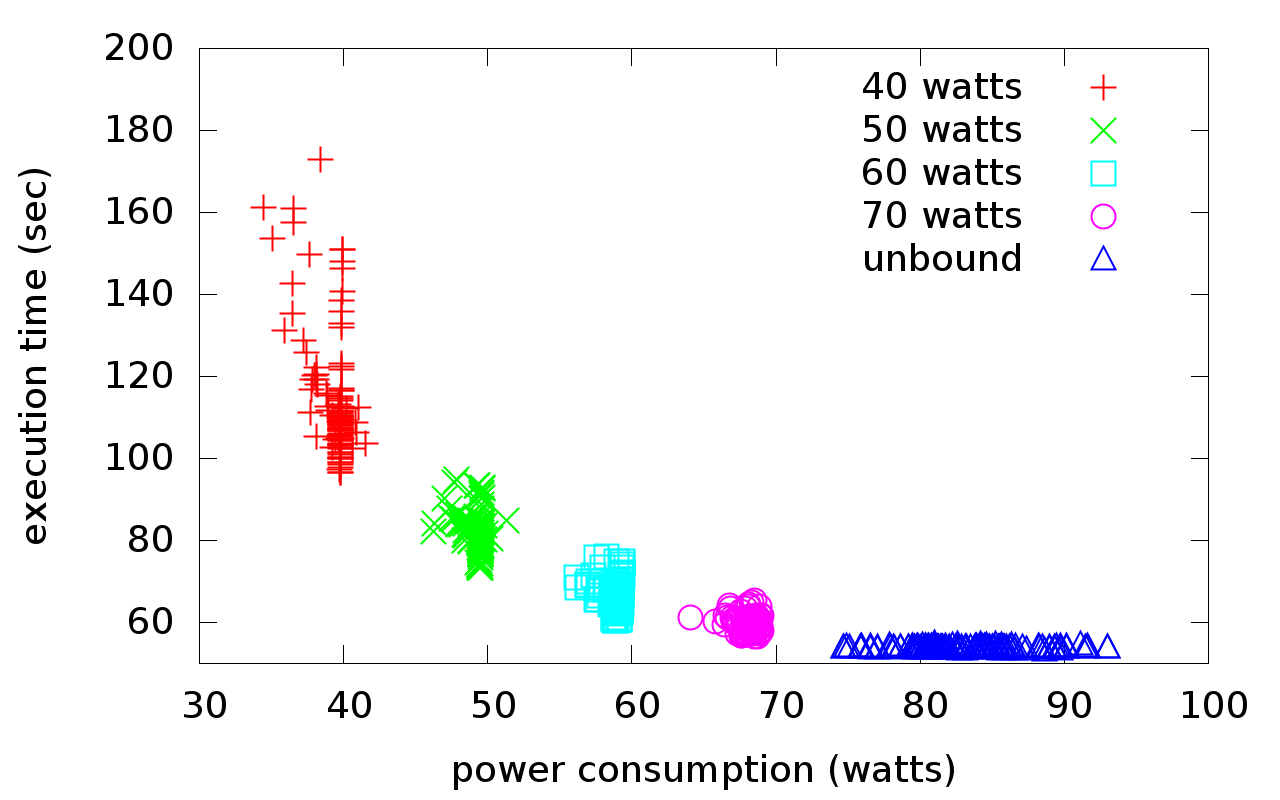
\includegraphics[width=\columnwidth]{background/figures/freqmine_power2perf_per_socket}
        \caption{Performance obtained when the \texttt{freqmine} application is run on 64 different 12-core Intel Xeon E5-2695v2 sockets under different power budgets.}
        \label{fig:socket_perf_variation}%
\vspace{.5cm}
\end{figure}

  


\section{A New Form of Heterogeneity}
%\subsection{A New Form of Heterogeneity}

HPC systems are becoming increasingly power hungry, as we keep pushing the boundaries of
performance on the road to exascale and beyond.  While significant advances have been made
in increasing the power efficiency of each single hardware component, i. e., flop/watt
ratios continue to decrease driven by significant architecture advances, these savings are
not enough to compensate for the growth in terms of computational elements required to
realize the needed performance advances.  Consequently, we need to build systems that use
power more efficiently and ensure that any power provisioned for a system is also used and
turned into realized performance, i.e., we need systems that can  dynamically manage their
power budgets among the available hardware components to direct power where it is needed.

Current machines are ``worst-case provisioned'', i.e., all components of a system can be
powered at the same time without reaching the system's power limit. Since applications
rarely keep all components occupied\footnote{It's a well known fact that many applications
only run at a fraction of peak performance --- often way below 10\%}, this conservative
approach leads to ``wasted power'', i.e., provisioned power that is not used. Prior
studies show that this wasted power can be up to 30\% of a system's power
rating~\cite{patki:2013:eho:2464996.2465009,conductor2015}. One solution is to reduce the
provisioned power to the expected average power consumption, or even lower, allowing
systems to exploit all available power, and, consequentially, allowing for larger systems
at the same total provisioned power. In such systems, which we refer to as
``overprovisioned systems'', though, we must cap power to avoid power spikes caused by
intermittent phases to exceed the provisioned power and with that endanger the operation
of the entire system.

Many current architectures either already provide such power capping mechanisms or have
them on their near term road map. However, such capping doesn't come for free: it impacts
performance, as show by the results of some initial experiments in
Figure~\ref{fig:socket_perf_variation}.  The graph shows timing and power consumption of
multiple runs of the \texttt{freqmine} code from the PARSEC benchmark
suite~\cite{bienia2008} on 64 nodes of the Lawrence Livermore National Laboratory (LLNL)
Catalyst cluster~\cite{llnlconfluence}, using 12 threads per execution.  \texttt{Freqmine}
has been adapted to use OpenMP-like task-based parallelism~\cite{Chasapis:2015:PEI:2836331.2829952} and runs in
the top of the Nanos++ (v0.7a) parallel runtime system~\cite{nanos}.  Since each node is
composed of two 12-core Intel Xeon E5-2695v2 sockets, our experiments involve 128
different 12-core sockets and each run is limited to one of these 128 sockets.  We
consider five different power bounds: 40, 50, 60, 70W and unlimited per socket.  The TDP
for each socket was 115W. The x-axis shows the measured power consumption for each
execution of the \texttt{Freqmine}  benchmark while in the y-axis we show the
corresponding execution time.  We can see that running without a power bound results in
almost no performance variation, but exhibits a wide spread of power consumption. Under a
power bound, this power variation is no longer possible and we can see a drastic impact on
performance variation instead.  Further, we can see that lower bounds result in higher
variations.

This behavior can be explained by manufacturing variability, which causes different
processors to exhibit different efficiencies. The consequence of this phenomena is,
though, that nominally homogeneous NUMA turn into heterogeneous systems when operated
under a power cap equally applied to each socket.  Since such irregular responses are due
to uncontrollable manufacturing issues, there is no way to now how a particular software
component while behave if run on several particular nodes unless it has been run there
before. 


\section{Mitigating Manufacturing Variability}
In order to mitigate this performance inhomogeneity caused by manufacturing variability,
current static load balancing and scheduling mechanisms are insufficient, since they are
only based on workloads and do not take into account dynamic variability.  Classical
dynamic work stealing and load balancing techniques may mitigate~\cite{Blumofe1999,
Blumofe1995, Ravichandran2011, Zheng2011} this problem under certain circumstances, but
they are not enough when dealing with complex codes with frequent synchronization points.
In the following, we illustrate the limitations of dynamic load balancing techniques on
power limited scenarios by means of two examples: one considering a code with no barriers
(Section~\ref{sec:nobarriers}) and another one with many (Section~\ref{sec:barriers}).  In
both examples, the considered applications belong to the PARSEC benchmark suite, but have
been adapted to use OpenMP task-based parallelism~\cite{Chasapis:2015:PEI:2836331.2829952} and executed  on top
of the Nanos++ (v0.7a) runtime system~\cite{nanos}.

\begin{figure}[ht]
  \begin{subfigure}{\columnwidth}
        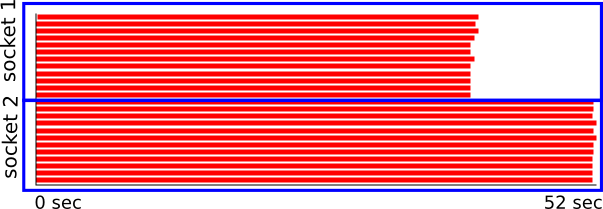
\includegraphics[width=\columnwidth]{power_aware_runtime/figures/swaptions-80watts-static}
        \caption{Static scheduling and 12 cores enabled.}
        \label{fig:swaptions_static_sched}
  \end{subfigure}
  \begin{subfigure}{\columnwidth}
        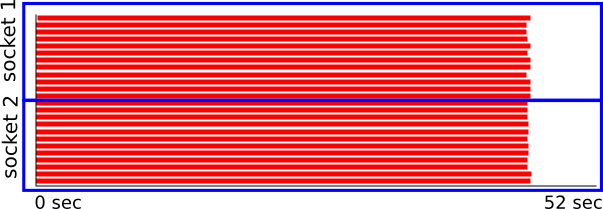
\includegraphics[width=\columnwidth]{power_aware_runtime/figures/swaptions-80watts-dynamic}
        \caption{Dynamic scheduling and 12 cores enabled.}
        \label{fig:swaptions_dynamic_sched}
  \end{subfigure}
  \caption{Executions of~\texttt{swaptions} 
                        under 40 W power capping.}
        \label{fig:load_balancing_sockets}
\vspace{.5cm}
\end{figure}



\subsection{Example with no Barrier or Synchronizations}
\label{sec:nobarriers}

\begin{figure}[ht]
  \begin{subfigure}{\columnwidth}
        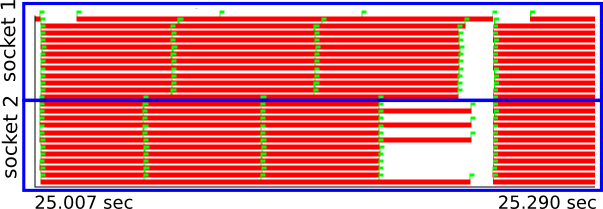
\includegraphics[width=\columnwidth]{power_aware_runtime/figures/blackscholes-80watts-even}
        \caption{Dynamic Scheduling and 12 cores enabled.}
        \label{fig:blackscholes_even_conf_trace}
  \end{subfigure}
  \begin{subfigure}{\columnwidth}
        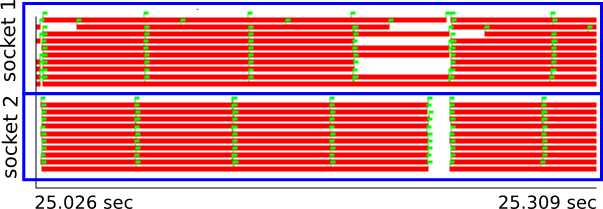
\includegraphics[width=\columnwidth]{power_aware_runtime/figures/blackscholes-80watts-best}
        \caption{Dynamic Scheduling and 10 cores enabled.}
        \label{fig:blackscholes_best_conf_trace}
  \end{subfigure}
  \caption{Executions of~\texttt{blackscholes} near a synchronization point under 40 W.}
  \label{fig:overprovisioning_sockets}%\
\vspace{.5cm}
\end{figure}


Figure~\ref{fig:load_balancing_sockets} compares two executions of the \texttt{swaptions}
benchmark~\cite{Chasapis:2015:PEI:2836331.2829952} on a NUMA node composed of two 12-core Intel Xeon E5-2695v2
sockets, each run with 24 threads and with power capped at 40W.  The x-axis of the figures
show time and the y-axis the activity of each of the 24 threads involved in the parallel
execution.  When the activity of a particular thread $i$ appears in red on time $t$, the
thread is doing useful work; if it appears in white, the thread is idling.  The scale of
the x-axis is the same in both figures and covers 0s to 52.8s.  In the run shown in
Figure~\ref{fig:swaptions_static_sched} the load is evenly distributed among all threads
statically using a naive distribution.  The reaction of the two sockets involved in the
parallel run is different, which makes the threads running on the faster socket (Threads
1-8) finish much earlier than the threads mapped to the slow socket (Threads 9-15). As a
result, threads from 1 to 8 are idle for 26\% of the execution time.

In Figure~\ref{fig:swaptions_dynamic_sched} we show a second parallel execution of the
same code, performed in the same NUMA node as above, but with dynamic scheduling.  For
this, we have over-decomposed the parallel execution into more tasks than cores and let
the parallel runtime system assign tasks to cores once they were idle.  In this way, the
cores on the fast socket executed some of the tasks that were assigned to cores on the
slower socket in the static case, which allows the whole parallel execution to achieve a
1.13x speedup over static scheduling.  This dynamic task assignment technique is
equivalent to the numerous work stealing approaches described in the
literature~\cite{Blumofe1999, Blumofe1995, Ravichandran2011, Zheng2011}: it is able to
deal with uneven hardware responses under restricted power budgets in the absence of
barriers or synchronization points.  Note however, that in order for conventional work
stealing to be effective, finer grain parallelism is prefered.  Introducing
synchronization and coarser parallel work unit limit the effectiveness of this method.


\subsection{Example with Barrier Operations}
\label{sec:barriers}

Figure~\ref{fig:overprovisioning_sockets} compares the behavior of two parallel executions
of the~\texttt{blackscholes} benchmark~\cite{Chasapis:2015:PEI:2836331.2829952} on the same NUMA node as the
one used above, again limited to 40W per socket.  In this case we show the behavior of the
parallel run around a barrier operation instead of the whole execution.  The x-axis
represents time and the y-axis shows the threads involved in the parallel execution.
Green flags mark the separation between the different pieces of sequential work in which
the parallel execution is split or, in other words, the tasks.

Figure~\ref{fig:blackscholes_even_conf_trace} shows the behavior of the dynamic task
scheduling using the same policy as above, with idle time shown in white.  While in the
absence of barriers this technique properly balances the load between the two 12-core
sockets, the results in this case clearly show that they fail in case of barriers: the
green flags show that the same tasks exhibit differences in execution time depending on
the socket they run on: around 74$\mu$s on average when run on the slow socket and 58 when
run on the fast one, despite each task executing the same computational workload.  Having
tasks with smaller granularity could offer more flexibility to the runtime's scheduler to 
better distribute the tasks among the sockets and cores, but it is not always possible to
decompose work into smaller units.  Furthermore, this requires alterations to the source
code of the application.  In this Chapter we propose a different approach to solve this
issue by redistributing power among sockets and finding the optimal concurrency level,
suitable for the specific socket and application.

Figure~\ref{fig:blackscholes_best_conf_trace} shows a second execution with the number of
threads per socket reduced to 10, i.e., 2 cores per socket or 4 cores total are left
unused during the execution.  In this example power is evenly distributed with 40W per
socket.  The average execution time of the tasks mapped to the slow socket gets reduced to
54$\mu$s, while the average time of those mapped to the fast socket takes 48$\mu$s to run.
This improved execution time is caused by the fact that the socket power budget is now
distributed among 10 cores instead of 12.  More importantly, the heterogeneous character
of the socket's response to the imposed power limit seems to be reduced by leaving 2 cores
idle.  This better balance between the two sockets significantly reduces the impact of
barriers and, therefore, their idle time.  Clearly, this is a much more balanced execution
than the one shown in Figure~\ref{fig:blackscholes_even_conf_trace}.  Overall, the
parallel run considering 10 cores per socket and dynamic task assignment shows a 1.21x
speedup with respect to the execution with 12 cores per socket combined with a dynamic
assignment.

This last example clearly shows that, under restricted power budgets and uneven hardware
reactions, operating with the maximum possible concurrency while dynamically balancing
load is insufficient since barrier points can introduce significant idling effects.  In
this cases, it can be better to restrict concurrency levels in order to homogenize the
hardware reaction to low power budgets.  Alternatively, it can also be helpful to unevenly
distribute the total power budget assigned to the multi-core sockets of a NUMA node in
order to compensate for varying processor efficiency, as we demonstrate in
Section~\ref{sec:static_analysis}.

\begin{figure}[ht]
        \centering
        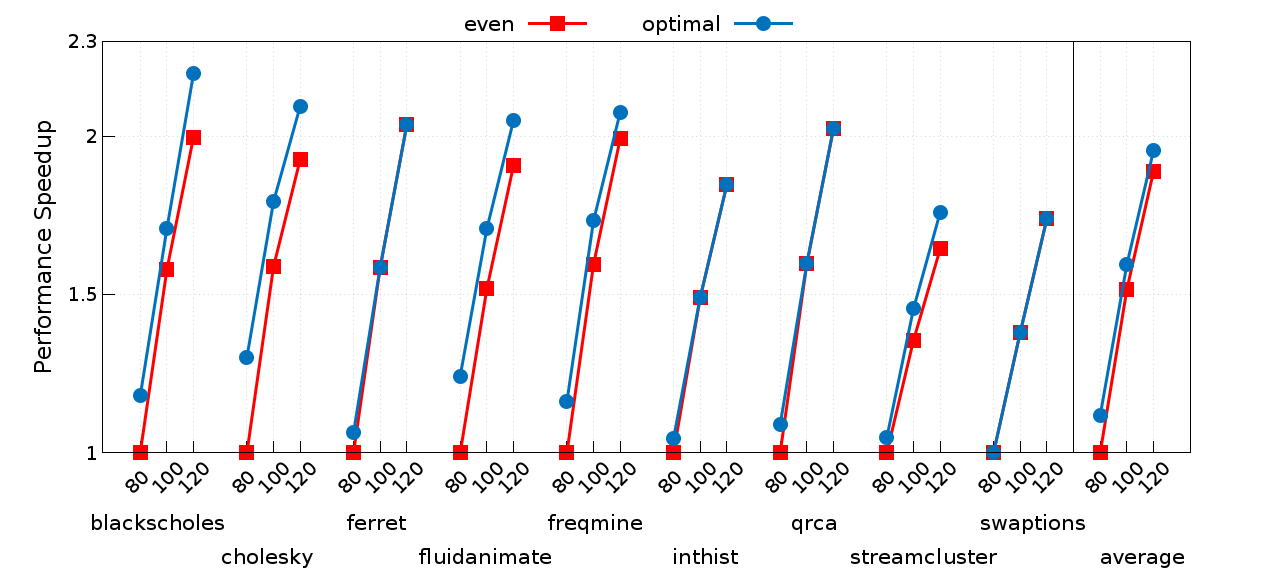
\includegraphics[width=\columnwidth]{./power_aware_runtime/figures/static_conf_analysis}
        \caption{Comparison between the even and the best configuration observed by application profiling. The speedup is computed over the execution of the even resource distribution for 80 W.}
        \label{fig:static_conf_analysis}
\vspace{.5cm}
\end{figure}


\begin{table}[]
\centering
\caption{Optimal configurations per application and power bound in terms or Watts and active cores per socket}
\label{table:optimal_configuration}
\def\arraystretch{1.5}%
\begin{tabular}{l|l|l|l|}
\cline{2-4}
                                    & 80 W & 100 W & 120 W \\ \hline
\multicolumn{1}{|l|}{\texttt{blackscholes}}  & 40-40 W, 10-10 cores & 55-45 W, 10-12 cores & 70-50 W, 12-10 cores \\ \hline
\multicolumn{1}{|l|}{\texttt{cholesky}}      & 30-50 W, 2-12 cores & 35-65 W, 2-12 cores & 30-90 W, 10-10 cores \\ \hline
\multicolumn{1}{|l|}{\texttt{ferret}}        & 40-40 W, 10-10 cores & 50-50 W, 12-12 cores & 60-60 W, 12-12 cores \\ \hline
\multicolumn{1}{|l|}{\texttt{fluidanimate}}  & 45-35 W, 10-6 cores & 55-45 W, 10-6 cores & 65-35 W, 10-6 cores \\ \hline
\multicolumn{1}{|l|}{\texttt{freqmine}}      & 45-35 W, 12-6 cores & 55-45 W, 10-12 cores & 65-55 W, 12-12 cores \\ \hline
\multicolumn{1}{|l|}{\texttt{inthist}}       & 40-40 W, 10-10 cores & 45-55 W, 12-12 cores & 60-60 W, 12-12 cores \\ \hline
\multicolumn{1}{|l|}{\texttt{qrca}}          & 45-35 W, 12-6 cores & 50-50 W, 12-12 cores & 60-60 W, 12-12 cores \\ \hline
\multicolumn{1}{|l|}{\texttt{streamcluster}} & 35-45 W, 2-12 cores & 60-40 W, 12-12 cores & 65-55 W, 12-12 cores \\ \hline
\multicolumn{1}{|l|}{\texttt{swaptions}}     & 40-40 W, 12-12 cores & 50-50 W, 12-12 cores & 60-60 W, 12-12 cores \\ \hline

\end{tabular}
\vspace{.5cm}
\end{table}


\section{Mitigating Heterogeneity}
\label{sec:static_analysis}
Following Sections~\ref{sec:nobarriers} and~\ref{sec:barriers}, which illustrate the
negative impact of heterogeneity introduced by power capping, we now provide a general
evaluation of the benefits of heterogeneity mitigation.  We consider a wide range of
parallel applications coming from many areas and we test their performance considering a
large range of power and concurrency configurations.  For each application and power
bound, we select the best configuration and compare its performance with the performance
obtained by deploying the naive even configuration --- assign half the power to each
thread and use all the available cores --- combined with traditional task scheduler and
balancer.


\subsection{Experimental Setup}
\label{sec:setup}
{\bf Applications:} we utilize nine OpenMP codes: six of them come from the PARSEC
benchmark suite~\cite{bienia2008, Chasapis:2015:PEI:2836331.2829952} (\texttt{black-scholes}, \texttt{ferret},
\texttt{fluidanimate}, \texttt{freqmine}, \texttt{streamcluster} and \texttt{swaptions}).
Two  of them are dense linear algebra routines (a cholesky matrix factorization,
\texttt{cholesky}, and a QR communication-avoiding code, \texttt{qrca}~\cite{Demmel1997})
and another one builds a histogram from a set of data points (\texttt{inthist}).  All of
these codes exploit task-based parallelism.  The benefits of using a programming model
which is coupled with a runtime system is that only the runtime needs to be modified to
accomodate our power budget and active core balancing algorithm, as well as the online
monitoring methodology.  Individual applications remain untouched, and the runtime handles
everything in a transparent manner.

{\bf Hardware and System Software:} NUMA nodes of the Catalyst
supercomputer~\cite{llnlconfluence} are composed of  two 12-core Intel Xeon E5-2695v2
sockets each. The applications run in top of the Nanos++ (v0.7a) parallel runtime
system~\cite{nanos}. We map one thread per active core.  To set power constraints and
measure power consumption on each socket, we use Intel's RAPL~\cite{IntelArcManual} .
These registers are accessed by our modified version of the Nanos++ runtime using the
libMSR library~\cite{libmsr}. 


{\bf Configurations:} We consider power bounds of 80W, 100W and 120W for total
node power.  This leaves 40W, 50W and 60W respectively per socket, which is 
between 35\% and 52\% of each socket's 115W TDP.
Although limiting socket power to 50\% or less may seem
aggressive, studies have shown that typical HPC workloads only use 60\%-85\% of
the available power on the socket \cite{Patki:2015:PRM:2749246.2749262}.  Moreover,
actual applications, such as the PARSECSs benchmarks, exhibit different
behavior at different execution stages.  As a result, an application may
reach its power peak for only a portion of its total execution.
Power limits above 50\% would have minimal impact on overall performance.
Furthermore,  there is a well established trend of an increase in manufacturing
variability in more modern processor models
\cite{Marathe:2017:ESP:3149412.3149421} and is expected to keep rising.  In
order for our study to be relevant for future processors, we choose a
configuration that creates enough variability between two sockets.  If we allow
a power limit of 80W, we consider 5 different ways of distributing the power
among the two sockets of the NUMA node: 30W:50W, 35W:45W, 40W:40W, 45W:35W and
50W:30W as well as 36 ways of specifying the maximum concurrency allowed in
each 2-socket NUMA node: 2-2, 4-2, 6-2, 8-2, 10-2, 12-2, 2-4, etc.  up to
12-12.  In total, this leads to a total of 180 combinations.  Similarly, when
allowing a power limit of 100W there are 8 ways of distributing it, which
combined with the 36 possible ways of distributing the concurrency, leads us to
a total of 324 combinations.  Similarly, when the total power budget reaches
120W, the total number of combinations is 468.  Overall, for each particular
application we have 972 different combinations.

{\bf Other Considerations:} The results of these experiments are machine dependent since
each particular 12-core socket reacts in a different way when a power limit is set.
Ideally, all  972 configurations per application should be executed on many NUMA nodes to
really account for many possible hardware reactions when a power limit is set.  However,
due to the size of our experimental campaign, we randomly chose a single 2-socket NUMA
node for each considered application and run all 972 combinations on it.  Although this
random choice can slightly influence the relative results between the benchmarks, the
general conclusions we extract from them remain unchanged.

\subsection{Evaluation}
\label{sec:static_evaluation}
In Figure~\ref{fig:static_conf_analysis} we show our experimental results.  On the x-axis
we represent all the considered applications and the three power bounds we consider: 80W,
100W and 120W.  In the y-axis we represent, for each particular application, the speedup
achieved over evenly distributing 80W among two sockets (40W per socket) and keeping 12
active cores per socket.  On average, the optimal configurations outperforms the totally
even distribution (50\% of the power and 12 cores per socket) by 11.8\% (80W), 7.3\%
(100W) and 7.6\% (120W).

Not surprisingly, the more restrictive the power capping is, the more beneficial the
optimal configuration becomes in terms of performance.  The uneven hardware reaction gets
exacerbated by restrictive power bounds, which gives more room for improvement when the
hardware is rebalanced by changing the power and concurrency assignation per socket.
Application-wise, the benefits are much larger for applications %with parallel schemes
composed of several execution phases separated by barriers, like \texttt{fluidanimate}
(24\% improvement) or \texttt{cholesky} (30\%).  On the other side, \texttt{swaptions}
does not get any benefit from our power rebalancing techniques since its lack of barriers
enables simple load balancing schemes to mitigate the hardware heterogeneous response, as
described in Section~\ref{sec:nobarriers}.

In Table~\ref{table:optimal_configuration} we list the optimal configuration for each
application and power bound.  As expected, for applications without barriers
(\texttt{swaptions} and \texttt{inthist}) the most balanced configurations (40W:40W and
12-12 active cores, 40W:40W and 10-10 cores respectively)  are optimal.  Since for these
applications the parallel runtime system successfully manages the load, there is no need
for system balancing by means of power or concurrency reassignment among the involved
threads.  On the other side, applications like \texttt{cholesky} or \texttt{fluidanimate}
do really benefit from leaving significant parts of the cores idle and rebalancing the
power accordingly.  Clearly, the hardware heterogeneity induced by setting a power bound
is not compensated by load balancing schemes delivered at the parallel runtime system side
and some concurrency and power rebalancing must be done to maximize the performance of
these applications.

This evaluation demonstrates that classical work stealing and load balancing techniques
are not able to compensate the heterogeneity induced by power capping, except for trivial
situations where a parallel code has no global barriers or synchronization points and the
size of the parallel work unit is small enough to allows versatile alternative scheduling
scenarios.  Since the potential benefits of power and concurrency rebalancing is up to
30\%, there is a need for developing techniques able to figure out the optimal
configuration within a single execution run. 



\section{Runtime Approach}

While the previous experiments demonstrate the potential benefits of unevenly setting up
the power caps and the number of active cores per socket in a power-constrained NUMA node,
these benefits are obtained under the huge cost of running each application multiple times
in the targeted NUMA node, each time with a particular power and active cores limit.
Further, the results obtained using extensive search on a particular NUMA node are not
applicable to another one since the hardware response to low power bounds are driven by
manufacturing variability and cannot be known in advance.  Also, deriving a particular
performance ratio per power bound among the sockets contained in a NUMA node is not enough
as different applications react in a different way to such variability.  It is thus
necessary to develop techniques able to quickly determine the optimal power-\# of cores
distribution for a particular software component and NUMA node.

We implement our method at the runtime level, since such systems offer load-balancing and
can be easily extended with additional functionality.  They are also widely used and
expected to play a significant role in future parallel architectures \cite{JSFI19,
Casas2015}. 


\subsection{Exploiting Application Structure}
Parallel codes often decompose loops or segments of serial code into multiple work units
that run in parallel.  While (at least to date) many codes follow the Single Program
Multiple Data (SPMD) approach where multiple cores execute the same code several times,
even more complex patterns, different repetitions of loops that iterate over similar sets
of data several times produce similar execution patterns.  As a consequence, codes almost
always exhibit a certain degree of repetitive behavior that can be observed either over
time or by considering the logical execution structure, which is composed of event
sequences~\cite{Isaacs2015, Totoni2014, Casas2010}.  This iterative nature of parallel
applications allows us to effectively guide the whole application behavior by observing
only small but significant portions of the parallel execution.  Our approach considers
execution segments and associates each with a particular power and number of active core
assignation per socket. To identify such a segment, the runtime tracks and identifies task
instances of the same task type. 
The intuition behind our approach is that same type tasks should behave in similar
fashion.   However, if tasks of the same type behave in an non-deterministic manner,
then our approach will fail to find a better configuration.
For example, in the case of \textit{blackscholes} we only
have one task type, thus this case is trivial.  However, in other applications, such as
\textit{ferret}, there are a few different task types.  For \textit{ferret} these are
\textit{t\_seg}, \textit{t\_extract}, \textit{t\_vec}, \textit{t\_rank} and
\textit{t\_out}.  The runtime can identify the type of an instance by the call site of the
taskified functions or user provided labels. Then, for a given monitoring window, the
runtime will identify all the task types running, but compare the execution time of the
tasks with the same type.  There are cases however that this may not be possible.  For
example if no tasks of the same type are found running on both sockets or if the tasks
of the same type run different workloads (their execution time varies beyond a
threshold, thus they  are not comparable), 
then the current monitoring window is discarded and move to the next
configuration.  This may cause the runtime to miss a good configuration, or even the
optimal one.
\par
Identifying representative segments of an application has been extensively studied, 
especially in the context of hardware simulation, where running the entire 
application is too slow.  Techniques such as the one presented by Sherwood et. al
\cite{Sherwood:2001:BBD:645988.674158} and the SimPoint 3.0 framework \cite{simpoints3}
could be employed for a more robust analysis and deal with the aforementioned issues. 
However, our approach exploits information already available to the runtime that can be 
accessed fast, minimizing the analysis' overhead. 
%makes it possible to
%explore many different configurations on representatives code sections in a single run,
%which can the be used in an online search.

\subsection{Search Algorithm}
\label{sec:algorithm}
The search algorithm aims to find the optimal power and total number of active cores
balance among the different sockets of a NUMA node.  It starts with evenly distributing
power and activating all cores and then progressively iterates over a set of power/\#cores
configurations and selects the best one.  Per each configuration, the targeted application
runs for a certain amount of time.  The particular amount of time each configuration runs
for is a parameter we call \textit{monitoring window}.  The smaller this parameter, the
shorter the exploration, but  the more chances of getting a non-optimal configuration
since the amount of time it has been trained for may not be representative of the whole
execution.  On the other hand, large window sizes significantly increase the chance of
finding the right configuration, but make the algorithmic search phase larger.

To characterize the performance achieved by each configuration we use a \textit{throughput
metric} defined as the number of tasks executed during the monitoring window each
configuration runs for.  This metric is well defined for all applications we consider in
this work (see Section~\ref{sec:setup}) and is particularly well-suited since it also
implicitly captures the amount of idle time spent by the active cores.  Further, it does
not imply a significant amount of measurement overhead if the task granularity is kept
over the tens of $\mu s$ threshold.  Although this metric is specific for task-based
codes, any other light-weight metric able to capture the amount of time spent doing useful
work would provide similar results for other kinds of applications or programming models.

During the first monitoring window, the runtime system measures the throughput of evenly
distributing power among the sockets and using all the available cores.  This is
considered the best candidate until a configuration providing larger throughput is
observed.  After each iteration we then compare the throughput for the current profile
with the best one.  If the current one is better, it becomes the new best and is used for
the subsequent comparisons.  This analysis continues until the search space is exhausted,
which may require more than one application run.  At the end of each run, if we have not
yet exhausted the search space, the runtime saves a checkpoint of the analysis state and
resumes it in a succeeding run.

Special care must be taken to make sure that we are considering monitoring windows that
constitute representative execution segments.  If two windows capture different task types
comparing them is not fair since different tasks have different execution times.  To
address this issue, we keep a set of task types for each different window.  If the task
sets collected during the best and current windows are not equal, it could mean that the
two configurations were run at a different stages of the application's execution.  We call
these incompatible profile results \textit{mismatching windows}.  When this occurs, we
ignore the current configuration without comparing it to the best and continue by checking
another configuration over the next monitoring window.  Special care need to be taken for
the first monitoring window.  If the first and second windows mismatch, we discard both
and retrain the first configuration.  This will continue until we capture a representative
segment of the application, meaning that two consecutive windows will be matching.

Note that different alternatives are available when dealing with mismatching windows.
However, for this work we employ the simplest case, which is to discard it.

 
\begin{figure*}[t]
        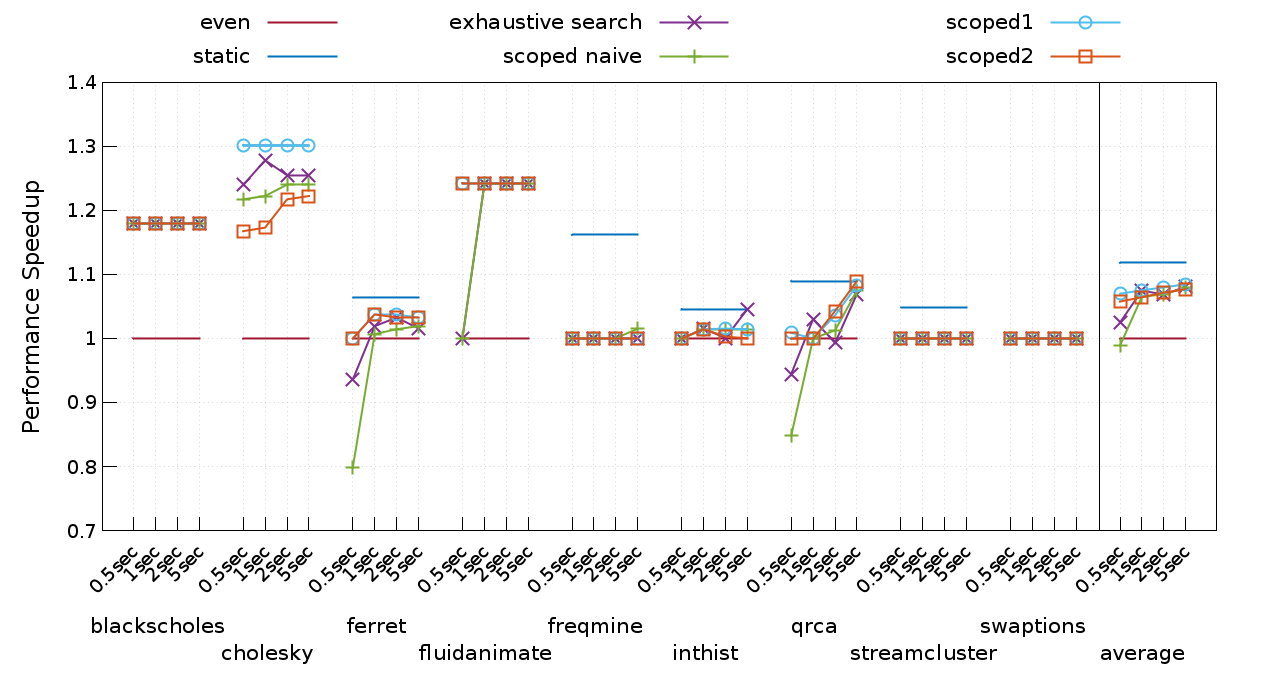
\includegraphics[width=\textwidth]{power_aware_runtime/figures/dynamic_window_impact}
        \caption{Comparison of best configuration found by exhaustive and scoped online analyses for different \textit{monitoring window} size, when running under a 80W power constraint.
                        The size of the monitoring window can influence the precision of the analysis.}
        \label{fig:mon_win_size_impact}%
\vspace{.5cm}
\end{figure*}



The search algorithm looks for the best configuration after trying several ones and
measuring their throughput over their corresponding monitoring windows.  As explained, the
monitoring windows size is an input parameter of our search algorithm.  The algorithm's
sensitivity to the windows size and its optimal value are explored in detail in
Section~\ref{sec:window_size_impact}.  Also, the set of configurations the search
algorithm iterates over is a key choice.  Large sets increase the chances of getting the
optimal power/\#active cores balance per socket, but also increases the cost of running
the search.  Alternatively, reduced sets may produce cheaper searches but also be unable
to find configurations that significantly improve performance. 

\subsection{Training Sets}
\label{sec:searchspaces}
We have implemented four variations of our analysis, based on the size of the configurations sets:

\textbf{Exhaustive Search:} We use the different configurations defined in
Section~\ref{sec:setup}.  As discussed above, in case we target a 80W power bound, the
exhaustive search considers 180 different configurations.  This is a conservative, but
expensive analysis. 


\textbf{Naive Scoped Search:} The scoped search does not consider extremely unbalanced
configurations since they rarely produce the most optimal results.  As a general rule we
focus the search on a small area around the default balanced configuration.  The reasoning
here is that just slightly providing more power or reducing the concurrency in the slower
socket will mitigate the imbalance between the sockets.  The scoped search considers 80
different configurations for the 80W bound.  They are composed of five different power
configurations (30W:50W, 35W:45W, 40W:40W, 45W:35W and 50W:30W) deployed for each one of
the 16 active core distributions: 6-6, 6-8, 6-10, 6-12, 8-6, ... , 12-12.

\textbf{Scoped Search 1:}
This training set aims to further reduce the search space, but considers both balanced and
unbalanced configurations.  It avoids irrational distributions like assigning more than
half of the power but less than half of the active cores to one of the sockets.  This
training set considers the even power configuration (40W:40W) and 9 different active cores
distributions for it: 8-8, 8-10, 8-12, 8-10, 10-10, 12-10, 8-12, 10-12 and 12-12.  It also
takes into account assigning 35W to the first socket and 45W to the second one with active
core counts 6-10, 6-12, 8-10 and 8-12 and its counterpart, that is, 45W to the first
socket and 35W to the second with active cores counts of 10-6, 12-6, 10-8 and 12-8.
Finally, this training set considers two unbalanced configurations: 30W:50W assigned to
the sockets and 2-12 active core counts per socket, and 50W:30W with 12-2 active cores.
This leaves us with 19 configurations when operating under the 80W power bound.

\textbf{Scoped Search 2:}
This training set contains the same distributions as Scoped Search 1 except the two
unbalanced configurations 50W:30W and 30W:50W, reducing the set to 17 configurations.
Very unbalanced configurations can produce large performance improvements, but also
increase the search costs since they significantly slowdown the execution in certain
cases.  This training set avoids the dangers of such unbalanced configurations by not
considering them. 

The reasoning here is that extreme configurations that greatly favor one socket or
severely reduce available parallelism are not likely to benefit an application.  Our goal
is to reduce the effect of the frequency imbalance between the sockets on a node, extreme
configurations would only benefit applications make sub-optimal use of the available
parallelism (e.g. dedup).


\section{Evaluation}

This section shows the results in applying our optimization technique.  The
experimental setup in terms of applications, system software and hardware is
the same as in section~\ref{sec:setup}.  For our evaluation we focus on an 80W
power budget (see \emph{Configurations} in Section \ref{sec:setup}). 

\begin{figure*}[p]
	\centering
        \begin{subfigure}{0.7\columnwidth}
        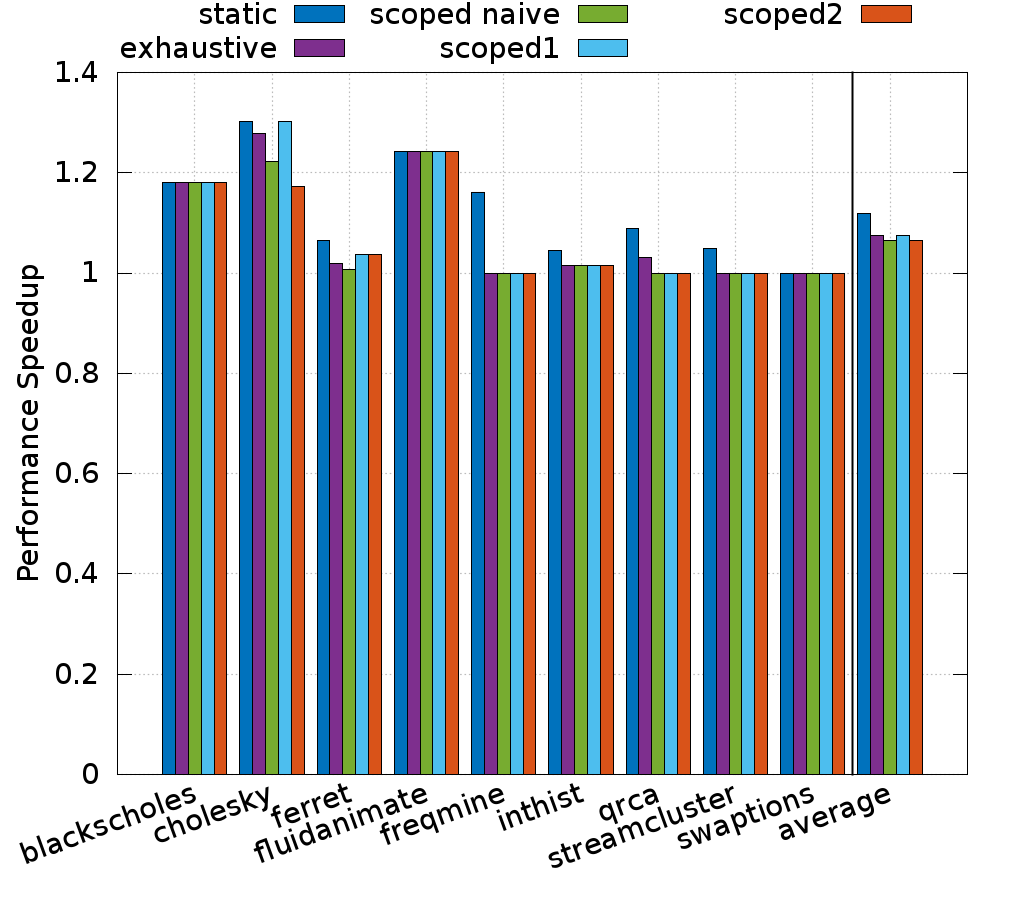
\includegraphics[width=\columnwidth]{power_aware_runtime/figures/dynamic_conf_performance_win1000000}
        \caption{Performance benefits of the selected configurations without accounting for the cost of the search.}
        \label{fig:net_benefit}%
        \end{subfigure}
        \hfill
        \begin{subfigure}{0.7\columnwidth}
        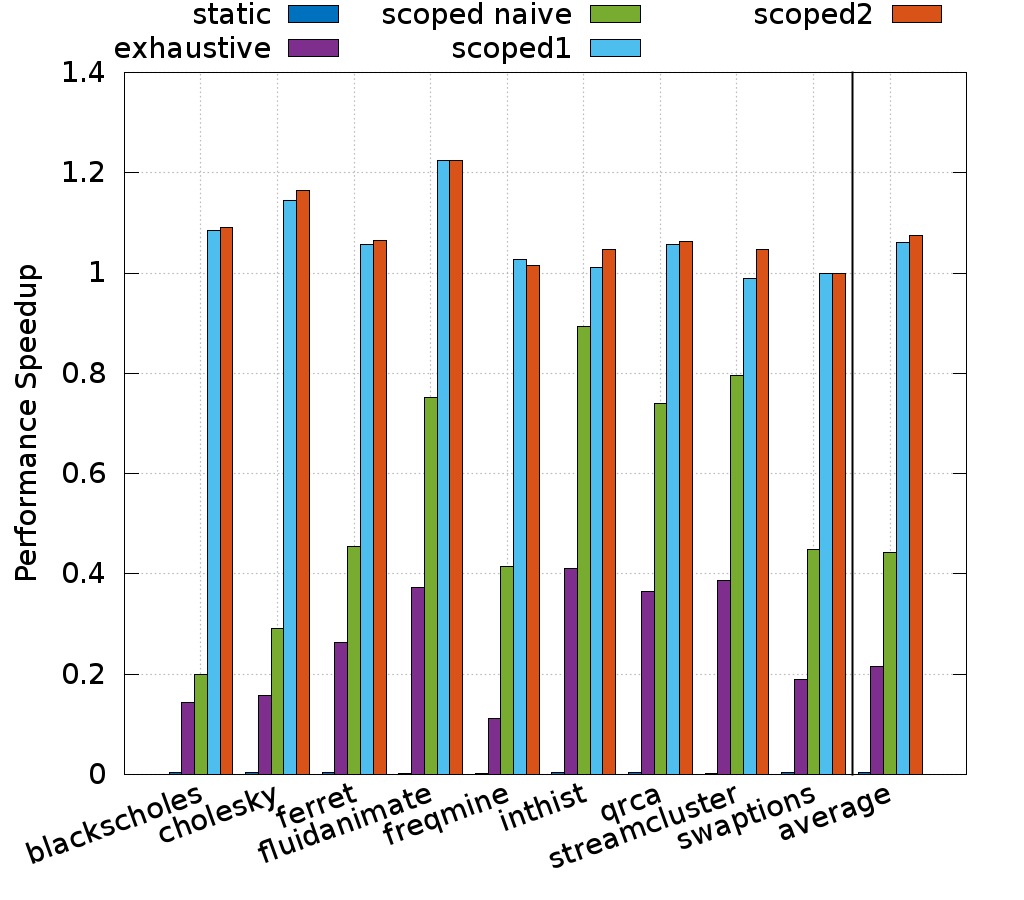
\includegraphics[width=\columnwidth]{power_aware_runtime/figures/dynamic_conf_cost_inv_win1000000}
        \caption{Performance benefits of the selected configurations taking into account the cost of the search.}
        \label{fig:dynamic_analysis_cost}%
        \end{subfigure}
        \caption{Performance benefits using monitoring windows of 1 second under 80 W power limit.}
\end{figure*}


\subsection{Monitoring Window Sensitivity}
\label{sec:window_size_impact}

This first section shows how an optimal window size is obtained by obtaining a detailed
sensitivity study.  This optimal size is leveraged in the following general evaluation of
the search algorithm in terms of its costs and benefits depending on the training set.


Figure~\ref{fig:mon_win_size_impact} shows how window sizes of 0.5, 1, 2 and 5 seconds
influence the effectiveness of the algorithmic search under an 80W power constraint.  The
x-axis represents the considered windows sizes for each application, while the y-axis
shows the speedups obtained over the trivially balanced configuration (40W and 12 active
cores per socket), represented in the figure with red horizontal lines.  The blue
horizontal line represents the speedups achieved by the optimal configuration found using
the multi-execution analysis presented in Section~\ref{sec:static_analysis} .  Purple and
green lines show results considering the exhaustive and scoped naive search spaces
described in section~\ref{sec:searchspaces}, while the blue and the orange lines represent
the scoped1 and scoped2 search spaces.  These results do not consider the cost of the
search algorithm, just the benefit of the optimal configurations found when using
different windows sizes and training sets.

Results shown in Figure~\ref{fig:mon_win_size_impact} clearly show that a windows size of
0.5 seconds on average does not provide  any gain when using the scoped naive training set
and only marginal gains when using the exhaustive search.  Indeed, the exhaustive and
scope naive searches bring significant performance degradations in cases like
\texttt{ferret} and \texttt{qrca} and fail in providing a configuration that delivers the
potential performance gains in case of \texttt{fluidanimate}.  When considering the
scoped1 and scoped2 training sets, 0.5 seconds window sizes do not provide significant
benefits in case of \texttt{ferret} and \texttt{qrca}.  On average, 0.5 seconds large
windows provide average speedups of 1.02x, 0.98x, 1.07x and 1.06x when exhaustive, naive
scope, scope1 and scope2 training sets are used.   

Increasing the windows size from 0.5 to 1 second improves the quality of the
configurations selected. 

Indeed, it provides speedups of 1.27x, 1.22x, 1.30x and 1.17x for \texttt{cholesky} or
1.24x, 1.24x, 1.24x and 1.24x for \texttt{fluidanimate} when exhaustive, trivial scoped,
scoped1 and scoped1 searches are used, respectively.  On average, the 1 second window size
provides benefits of 1.08x when exhaustive search is used and 1.07x when the trivial scope
set is considered, 1.08x when the scope1 is considered and 1.07x for the scope2.  As a
reference, when running a whole execution per each configuration we get optimum power and
active core distribution that bring average speedups of 1.12x.  Increasing the windows
sizes to 2 and 5 seconds does not significantly improve the results quality although they
asymptotically get closer to the ones obtained using the multi-execution analysis.  In
conclusion, the 1 second window size is the optimal one since it provides similar benefits
for all the considered training sets as the 2 and 5 second window sizes under a lower
cost.

The search algorithm works very well for applications with regular computations separated
by barriers (\texttt{blackscholes}, \texttt{fluidanimate} or \texttt{cholesky}) since each
monitoring window can capture different iterations of the same behavior.  In case of
\texttt{ferret} or \texttt{qrca} the scarcity of barriers or synchronization points
reduces the potential gains of our techniques.  When computations are more irregular, it
is more challenging to have consistent monitoring windows, which reduces the effectiveness
of our scheme.  In the particular case of \texttt{freqmine} the task type that accounts
for more than 90\% of the execution is input dependent and actually a single instance of
this task type can take up to half of the total execution time.  As a result the vast
majority of the considered configurations are dismissed since their corresponding
monitoring windows either mismatch or fail to capture any information.

\begin{figure*}[p]
				\centering
        \begin{subfigure}{0.7\columnwidth}
        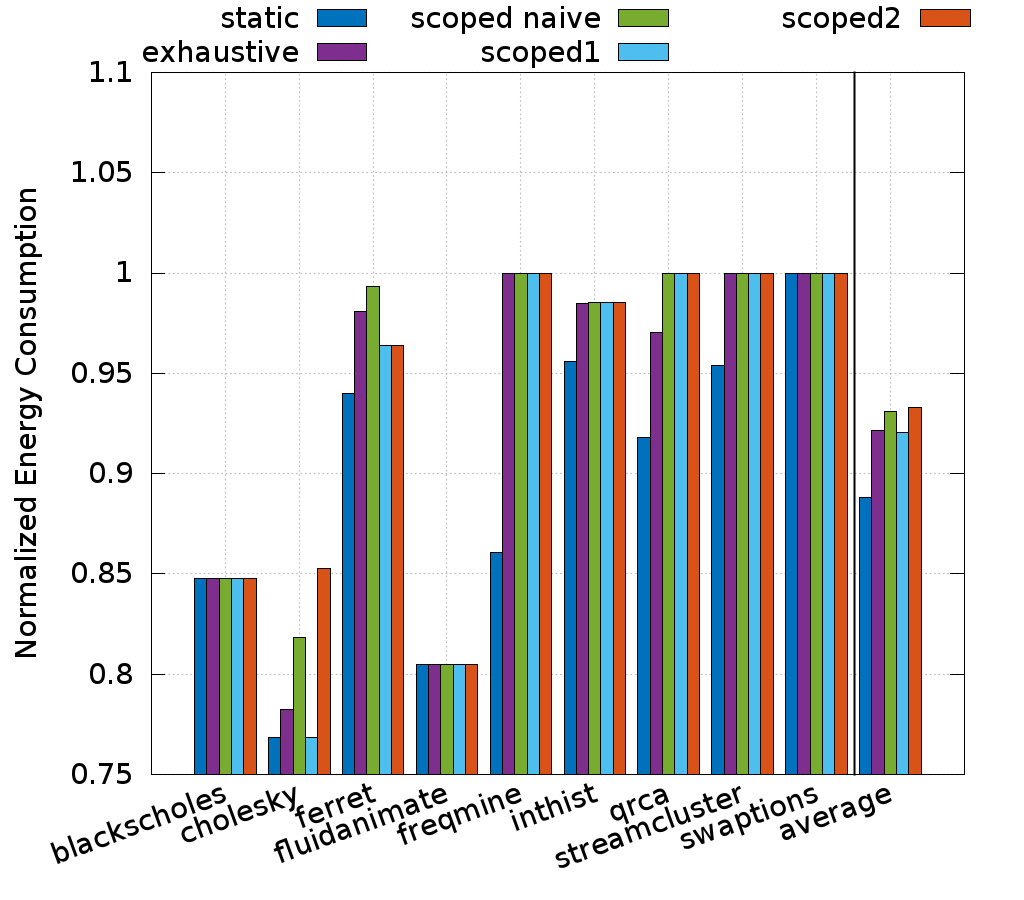
\includegraphics[width=\columnwidth]{power_aware_runtime/figures/dynamic_conf_energy_consumption_win1000000}
        \caption{Energy reductions of the selected configurations without accounting for the cost of the search.}
	\label{fig:dynamic_analysis_energy_consumption_no_cost}
        \end{subfigure}
	\hfill
        \begin{subfigure}{0.7\columnwidth}
        \includegraphics[width=\columnwidth]{power_aware_runtime/figures/dynamic_conf_energy_consumption_w_cost_win1000000}
        \caption{Energy reductions of the selected configurations taking into account the cost of the search.}
        \label{fig:dynamic_analysis_energy_consumption_w_cost}
        \end{subfigure}
        \caption{Energy consumption reduction using 1 second monitoring windows under a 80 W power bound.}
        \label{fig:dynamic_analysis_energy_consumption}
\end{figure*}

\subsection{Performance Improvements of the Selected Configurations}
In Figure~\ref{fig:net_benefit} we show in detail the performance benefits provided by the
optimal configurations found by each one of the four training sets considering a 80W power
bound and 1 second long monitoring windows.  The results are expressed in terms of speedup
with respect to the execution time when using the naive even distribution (40W:40W and
12-12 active cores).  The static technique consists of entirely running the applications
for each one of the 180 configurations defined in Section~\ref{sec:setup}.  The results of
the static technique have already been presented in Section~\ref{sec:static_evaluation}.
This technique, while prohibitively expensive in practice as it requires 180 runs per
application, always finds the best possible configuration and hence provides an upper
bound of the speedup possible. We represent its results in Figure~\ref{fig:net_benefit}.

In case of \texttt{blackscholes} and \texttt{fluidanimate}, all the training sets
(exhaustive, naive scoped, scoped 1 and scoped 2) find configurations that provide the
same speedup as the static technique, 1.17x and 1.24x respectively.  In case of
\texttt{cholesky}, the exhaustive and scoped 1 training sets allow the system to find
configurations that provide speedups very close to 1.3x, the best possible one.  The naive
scope and scoped 2 techniques provide speedups close to 1.2x.  Although these benefits are
significant, they are far from the ones achieved by the other techniques.  The reason is
that the \texttt{cholesky} application benefits a lot from unbalanced distributions
(Table~\ref{table:optimal_configuration}), which are neither considered by the naive scope
nor by the scoped 2 training sets.  In case of \texttt{freqmine}, although the optimal
identified configuration by the static analysis does provide significant benefits, the 4
training sets considered by the searching algorithm fail in finding this optimal
configuration, since tasks are input dependent and can take up to half of the execution
time, as a result most windows fail to capture task throughput since not tasks finish
execution.  In case of \texttt{ferret}, \texttt{inthist}, \texttt{qrca} and
\texttt{swaptions}, the potential benefits of power and active cores balancing are very
limited, since these applications do not have a significant number of barrier
synchronizations.  As we have explained in Section~\ref{sec:nobarriers}, when the overall
number of barriers is not significant, classical load balancing mechanisms are enough to
maximize performance under low power scenarios.

On average, all  training sets provide benefits of around 1.07x, while the static
technique provides an average speedup of 1.11x.  The training costs of the five approaches
are not considered in Figure~\ref{fig:net_benefit}.

\subsection{Performance Improvements Taking into Account Analysis Costs}
\label{sec:costs}
All considered techniques require an analysis to find a power/active cores balance that
optimally improves the trivially balanced distribution.  This analysis starts once the
execution of the parallel code begins and finishes when all the considered configurations
have been tested.  If a single application run is not sufficent to test all the
configurations of the training set, the application is run again and again until the
training is complete.

Figure~\ref{fig:dynamic_analysis_cost} shows the speedups achieved by all considered
techniques including the training phase costs.  In case of the static analysis it is
required to run the application multiple times, one per each of the 180 different
power/active cores distributions.  Consequently, the overall speedup is 0.003x, much
smaller than 1x.  The exhaustive training set considered 180 distributions and checks
their performance over monitoring windows that are 1 second long.  Therefore, more than
one run is required to test all the configurations for those applications with execution
times smaller than 180 seconds.  Since this is the case of all the considered parallel
codes, the average speedup achieved by the exhaustive training set is 0.21x.  Similarly,
the trivial scoped training set obtains a speedup of 0.44x.  These three techniques do not
improve the trivial approach which consists in just evenly distributing the total
available 80W power budget and using all the cores available in the 2-socket NUMA node.

The scoped 1 and 2 training sets consider much fewer configurations than all  previously
mention approaches and, therefore, their training costs are significantly smaller.
Indeed, they are able to test all configurations for 1 second, select the best one and
then run the rest of the application using this optimal configuration.  Of course, the
cost of the training phase can reduce the overall benefits of the optimal configuration,
as it is the case of \texttt{blackscholes}, where the benefits of the scoped 1 and 2
training sets are reduced from 1.17x to 1.08x and 1.09x respectively.  \texttt{Cholesky}
and \texttt{fluidanimate} have larger execution times than \texttt{blackscholes}, which
allows them to compensate the cost of the training phase when scoped 1 and 2 training sets
are considered and to keep almost the same performance gains as if the training costs were
not considered (1.15x and 1.22x, respectively).

Finally, Figure~\ref{fig:dynamic_analysis_cost} reports marginal performance benefits for
some applications for which the search algorithm does not find any distribution
significantly better than the trivial.  For example, in case of \texttt{qrca} there are
speedups of exactly 1x in Figure~\ref{fig:net_benefit}, but of 1.05x and 1.06x for scoped1
and scoped2 in Figure\ref{fig:dynamic_analysis_cost}.  The explanation of this behavior is
that, although the search algorithm fails to find any configuration that is significantly
better than the evenly distributed, there are indeed many configurations that perform
slightly faster than the even one, which accelerate the execution as they are used during
the training phase.

Overall, the static technique and the exhaustive and trivial scope training sets produce
an overall performance slowdown, which makes these approaches useless in practice.  On the
other hand, the scoped 1 and 2 training sets provide important performance benefits even
when the search phase is taken into consideration, which makes these approaches very
useful to maximize performance in power constrained scenarios.

\subsection{Energy Consumption Reductions}
\label{sec:energy}
Figure~\ref{fig:dynamic_analysis_energy_consumption_no_cost} shows the energy consumption
reductions achieved when using configurations found by the five different techniques if
training costs are not considered.  The baseline is the energy spent by the trivially
balanced configuration (12 active cores and a maximum of 40W per socket) and all results
are normalized to this baseline.  The configurations selected by the static analysis
provide energy reductions of 11\% with respect to the even distribution since the
normalized energy gets reduced from 1 to 0.89.  The reductions provided by the search
algorithm are between 7\% and 8\%, depending on the training set.

Once the cost of the exploration phase is considered, the energy consumed by the static
analysis, the exhaustive and the scope naive training sets are 295, 3.7 and 1.8 times
larger than the energy consumed by a single run with the even configuration.  In
Figure~\ref{fig:dynamic_analysis_energy_consumption_w_cost} we just represent normalized
energy consumptions below 1.1 for readability purposes.  As observed before, the scoped 1
and 2 training sets are able to compensate the cost of the training set and deliver
improvements over the even configurations.  The energy consumption reductions are 0.94 and
0.93 for the scoped 1 and 2 training sets respectively.


\section{Summary}
In this Chapter we demonstrate how state-of-the-art parallel runtime systems can mitigate the performance imbalance between sockets on the same node when
operating under strict power constraints.  We establish that load-balancing, although improving performance, is not sufficient for a wide set of applications.  In our study
we use six applications from the PARSEC benchmark suite and three additional applications, all implemented with OpenMP 4.0 tasks.
The OpenMP runtime offers us a perfect platform for developing our methodology, without the need to
any additional modification for each application.
By performing profiling runs of 
the applications with different power distributions and active number of cores on each socket we demonstrate that it is possible to achieve speedups up to 1.30x over
naively spreading evenly the power budget and using all possible cores.
%
We also propose and implement an online analysis that monitors only a segment of the application's execution and is able to
switch between different power and concurrency configurations at runtime, reducing the overhead of profiling.  
Our evaluation shows that it is possible to carefully compose the configuration search space by eliminating candidates that are unlikely to give a good result (such as reducing
power but increasing concurrency). 
The online analysis achieves speedups up to 1.22x over the naive case.

This work focused on figuring out the optimal power-concurrency balance on machines with 2 sockets per NUMA
node, which is a common setup in current systems. Future configurations will have many more sockets on a single node. 
In respect to our method this trend will likely require increasing the training set sizes, thus the cost and its complexity. 
However, the benefits of our technique will also increase: more sockets imply an even more varied response to low power scenarios within the same NUMA node.
Adding accelerators will further increase the number of frequency/power capping domains. By restricting our searches to well-balanced configurations, as shown 
in this work, we can avoid a combinatorial explosion in the training set sizes, which keeps training costs within reasonable margins and enables larger performance 
improvements on multi-socket NUMA nodes. The results on 2 a socket system, as described in the thesis, therefore cover the worst case scenario.

 



\chapter{Power-Aware Job Scheduling}
\label{chap:power_aware_job_scheduling}


Power is becoming a major financial and environmental concern, restricting the compute
capacity of High Performance Computing (HPC) systems.  Today's most power efficient
supercomputer operates at 14.1GFLOPS/W~\cite{Green500:2017}, but even if we had a system
able to operate at the 50GFLOPS/W rate, which is the limit that some funding agencies have
set up for building an exascale machine, the full system would consume several tens of
MWatts of power, which constitutes a large economic burden.  Consequently, a report from
the US Department of Energy (DOE)~\cite{ASCAC:tech:2014} identifies energy efficiency as
one of the top ten research challenges on the road to exascale.  For similar reasons, the
European Union has set up an HPC program % is also concerned and focused on building
low-power systems based on mobile technology~\cite{Rajovic2013}.
\par
An emerging design practice for HPC systems, known as 
\textit{overprovisioning}~\cite{patki:2013:eho:2464996.2465009}, is to have more nodes
than the maximum power budget could feed if run at peak capacity, in contrast to
traditional approaches, which are focused in having enough power even when all nodes run
at their peak. Overprovisioning is driven by the observation that most applications in 
practice never reach peak power and hence do not fully utilize the available power envelope. 
In such overprovisioned systems, we can lower the average power provisioned to each node, 
allowing us to power more nodes within the same power budget. This approach is made possible 
by recent developments in hardware design that enable power management and power capping from 
user space, as this is necessary to efficiently manage power as a limited and shared resource. 
As an alternative to restricting power to nodes, we can choose to only operate fewer but at 
full power. Their total power consumption should not exceed that of the total power budget. 
This second approach restricts the available parallelism in the system, but allows for faster 
execution and does not force us to deal with any complications related slower then expected 
execution of the system’s workload. Which approach is preferable (or a combination of both) 
should depend on system and workload characteristics. For example, whether the workload would 
benefit from extra processing units or limitations in the completion time set by the user
or administrator.
\par
Workloads at the HPC system level  are managed by job schedulers that allocate resources
to dispatched jobs.  Such jobs can run on distributed memory scenarios and, in this
context, MPI~\cite{Nagle:2005:MCR:1239662.1239666} is the most common approach to handle
distributed memory communications.  It is usually coupled with a shared memory programming
model, like OpenMP~\cite{openmp13} or similar~\cite{10.1007/978-3-540-85261-2_5}.
Either across nodes or within a shared-memory node, both job and runtime schedulers deal
with the resource allocation problem, albeit at different levels, offering opportunities
to manage power consumption.  Indeed, examples of power-aware systems  that offer
solutions either at the job scheduling
\cite{Gholkar:2016:PTH:2967938.2967961,7515666,Ellsworth:2015:DPS:2807591.2807643,Etinski2012615}
or at runtime system  \cite{Gholkar:2016:PTH:2967938.2967961,
Chasapis:2016:RMM:2925426.2926279,Totoni:tech:2014,Teodorescu:2008:VAS:1381306.1382152,Inadomi:2015:AMI:2807591.2807638}
levels already exist in the literature.
\par
Manufacturing variability or process variation refers to the power and frequency
heterogeneity observed across chips implementing the exact same architecture as a
consequence of uncontrollable material differences in the manufacturing
process~\cite{Rountree:2012:BDF:2357488.2357648}.  In order to provide homogeneous
performance, chips of the same architecture must hide frequency variability, which can
only be achieved via variations in their power consumption.  However, in a power
constrained environment where all chips need to operate under a certain power cap, this
frequency variability can no longer be hidden~\cite{Rountree:2012:BDF:2357488.2357648},
leading to heterogeneous performance.  As a result, a theoretically homogeneous system
turns into a heterogeneous one with performance variations of up to
64\%~\cite{Inadomi:2015:AMI:2807591.2807638}.  While ignoring this manufacturing
variability leads to performance and energy inefficiencies, there are opportunities for
achieving improvements at the power budgeting or parallel runtime system levels when
variability is properly
managed~\cite{Chasapis:2016:RMM:2925426.2926279,Teodorescu:2008:VAS:1381306.1382152,Inadomi:2015:AMI:2807591.2807638,Gholkar:2016:PTH:2967938.2967961,Totoni:tech:2014}.

\begin{figure}
	\centering
	\includegraphics[width=\columnwidth]{power_aware_job_scheduling/figures/motivation}
	\caption{Total power consumption trace for Conservative, Variability agnostic and 
		Variability aware scheduling policies, when running the same workload.  
		Considering socket variability maximizes performance 
		and meets the power budget.}
	\label{fig:motivation}
	%\vspace{-.3cm}
\end{figure}

\par
This thesis goes beyond the state-of-the-art by proposing job scheduling policies driven by
variability-aware power prediction models.  We consider two different approaches to
predicting manufacturing variability.  The first model assumes that all applications
are affected the same way by manufacturing variability.  This assumption is not correct, as 
demonstrated in Section \ref{sec:model_validation}. The second model offers a more robust
approach, where the model uses a training set of applications to identify how different application
behavior is impacted by manufacturing variability.
We extend power-aware scheduling and power
prediction models to deal with manufacturing variabity,  producing two novel variability-
and power-aware job scheduling policies.  The goal of these policies is to maximize the
utilization of the cluster without exceeding the available power budget and without
restricting per socket power consumption.  Instead, by using the power prediction, the
policies can find the maximum number of concurrent jobs that can run within the power
budget.  This offers an alternative to per node power capping, which in combination with
manufacturing variability, would create an heterogeneous cluster.  Current workload
managers do not account for this type of heterogeneity.   
We consider the power consumption of the CPU,
since it accounts for more than 50\% \cite{ShuaiwenSong:2009:EPA:1572226.1572228} of the
total node's power consumption.  Our Policies rely on two different models and leverage
their power requirement predictions of individual parallel jobs to make scheduling
decisions that maximize performance while reducing energy consumption.  Many different
variability-agnostic power and energy prediction models have been proposed
~\cite{Bircher:2012:CSP:2196827.2196987,Bertran:2012:SEC:2457472.2457499,Bertran:2010:DRP:1810085.1810108,Goel:2010:PSP:1909624.1909734,Isci:2003:RPM:956417.956567}
	and are often employed to manage power distribution on clusters to mitigate the effects of
manufacturing variability
~\cite{Chasapis:2016:RMM:2925426.2926279,Inadomi:2015:AMI:2807591.2807638,Gholkar:2016:PTH:2967938.2967961,Ellsworth:2015:DPS:2807591.2807643,Bailey:2015:FLP:2807591.2807637,Teodorescu:2008:VAS:1381306.1382152,Totoni:tech:2014}.
\par
As a motivation we show Figure~\ref{fig:motivation}, where three different scheduling
policies are compared.  The Conservative simply considers that all jobs consume the same
power on all sockets.  The Variability agnostic predicts accurately the power consumption
of individual jobs, but does not consider socket variability.  On the contrary, the
Variability aware policy does also consider socket variability, making a different
prediction per socket.  As displayed in Figure~\ref{fig:motivation}, the Conservative policy is
the one providing the worse performance. The Variability agnostic improves performance by
making more accurate predictions but fails to account for the more power consuming
sockets, exceeding the 15KWatts power budget.  Finally,  the Variability aware policy
manages to improve performance, while respecting the power budget.  
Figure~\ref{fig:motivation} illustrates how accounting for manufacturing variability while scheduling parallel jobs provides performance benefits.
Section~\ref{sec:experimental_setup} describes the experimental setup we consider to generate Figure~\ref{fig:motivation}.

%Precise knowledge of
%the power consumption of individual jobs on all available sockets, while considering their
%avialability can have a significant impact in performance and optimize power utilization.
\par
This thesis shows how variability-aware power prediction models can be effectively used to
guide job scheduling policies and bring significant benefits with respect to the
variability-agnostic ones.
In particular, this thesis makes the following contributions beyond the state-of-the-art:
\begin{itemize} 

	\item Two new variability-aware power prediction models. 
				Both models use Performance Monitoring Counters (PMC) to
				predict an application's 
				power consumption on a specific socket.
				PMCs are used to measure the activity of individual architectural components while 
				the targeted application is running and a linear model is then used to find their 
				contribution to power consumption.
				The first model assumes power variability to impact all applications equally.  
				It uses a single benchmark to measure the power consumption variability across 
				sockets and apply it to the variability agnostic PMC-based model.  
				The second model extends the PMC-based approach to take power consumption 
				variability into account, as part of the model.  It trains the model for each 
				individual socket, using a reduced set of benchmarks.

	\item Two power- and variability-aware job scheduling policies that optimize job 
				turnaround time and energy efficiency while respecting a system-wide power budget.  
				Unlike previous work that does not consider variability during job scheduling 
				decisions~\cite{Inadomi:2015:AMI:2807591.2807638,Teodorescu:2008:VAS:1381306.1382152,Ellsworth:2015:DPS:2807591.2807643,Gholkar:2016:PTH:2967938.2967961}, 
				our policies use variability-aware predicton model to guide scheduling.

	\item A complete evaluation of the two variability-aware policies via a discrete event 
				simulator.  We implement additional scheduling policies for our evaluation, which 
				represent traditional and state-of-the-art  practices used in today's HPC systems.  
				Our evaluation demonstrates how variability-aware policies achieve energy savings 
				up to \MaxEnergy\% and job turnaround time reductions up to \MaxJTT\%, considering 
				different power budgets and two workload traffic scenarios (bursty and heavy).
\end{itemize}    	

The remainder of this Chapter is organized as follows.
Section~\ref{sec:variability_prediction} presents the two variability-aware power
prediction models.  Section~\ref{sec:job_sched_scheduling} introduces the variability and
power-aware scheduling policies we propose.  A validation of the models and evaluation of
our job scheduling policies are presented in Section~\ref{sec:job_scheduling_results}
and, finally, Section~\ref{sec:job_sched_conclusions} provides summarizes the
ideas and results presented in the Chapter.


\begin{table}
	\centering
	\caption{Architectural component activity ratios formulas for Intel \ARCH~Architecture,
inferred from Intel's 64 and IA-32 Architectures Software Developer's Manual
\cite{fquesnel:progguide:intel10}}
	\label{tab:comp_formulas}
	\begin{tabular}{ | c | m{10cm} | } 
		\hline
		\textbf{Power Component} & \textbf{Component Activity Formula} \\ 
		\hline
		\hline
		Fetch & UOPS\_RETIRED.ALL / CPU\_CLK\_UNHALTED.THREAD\_P \\ 
		\hline
		Branch Prediction Unit & BR\_INSTR\_RETIRED.ALL\_BRANCHES / CPU\_CLK\_UNHALTED.THREAD\_P \\ 
		\hline
		Arithmetic \& Logic Unit & (UOPS\_DISPATCHED\_PORT.PORT\_0 + UOPS\_DISPATCHED\_PORT.PORT\_1 + UOPS\_DISPATCHED\_PORT.PORT\_5) / CPU\_CLK\_UNHALTED.THREAD\_P \\ 
		\hline
		Floating Point & FP\_COMP\_OPS\_EXE.X87 / \newline CPU\_CLK\_UNHALTED.THREAD\_P \\ 
		\hline
		L1 cache & L1D\_ALL.REF / CPU\_CLK\_UNHALTED.THREAD\_P \\ 
		\hline 
		L2 cache & (L2\_RQSTS.ALL\_RFO + \newline L2\_RQSTS.ALL\_DEMAND\_DATA\_RD) / \newline CPU\_CLK\_UNHALTED.THREAD\_P \\ 
		\hline	
		L3 cache & LLC.References / CPU\_CLK\_UNHALTED.THREAD\_P \\ 
		\hline
		Memory & LLC.Misses / CPU\_CLK\_UNHALTED.THREAD\_P \\ 
		\hline
	\end{tabular}
%	\vspace{-.5cm}
\end{table}



\section{Power Variability Prediction Models}
\label{sec:variability_prediction}

Power modeling has received a lot of attention from researchers and developers as it
provides a quick and robust way to understand the power behavior of a system.  A common
approach for predicting power consumption consists in the usage of Performance Monitoring
Counters
(PMC)~\cite{Bertran:2010:DRP:1810085.1810108,Singh:2009:RTP:1577129.1577137,Bellosa:2000:BED:566726.566736,Bircher:2012:CSP:2196827.2196987,Bircher:2005:RIM:1077603.1077668,Li:2003:RME:781027.781048},
since sampling PMC does not introduce significant power
interference~\cite{Joseph:2001:RPE:383082.383119,Isci:2003:RPM:956417.956567} and
PMC-based prediction models decompose a chip into several components in terms of power
consumption~\cite{Bertran:2010:DRP:1810085.1810108}.  While power prediction models are
employed to find the best tradeoff between power and
performance~\cite{Gholkar:2016:PTH:2967938.2967961}, we are not aware of any previous work
that uses variability-aware power models to guide job scheduling decisions.  

%In the rest of the document, we consider a cluster to consist of multiple nodes, each with
%multiple sockets. Thus, the terms socket and CPU are used interchangeably.


\subsection{Power Ratio Model}
\label{sec:naive_model}

\begin{figure*}[!ht]
	\centering
\begin{subfigure}[b]{.45\textwidth}
  	\includegraphics[width=\textwidth]{power_aware_job_scheduling/figures/activity_ratios/blackscholes_pkg_power}
  \end{subfigure}%
~
	\begin{subfigure}[b]{.45\textwidth}
  	\includegraphics[width=\textwidth]{power_aware_job_scheduling/figures/activity_ratios/bodytrack_pkg_power}
	\end{subfigure}%
\vspace{0.1cm}
	\begin{subfigure}[b]{.45\textwidth}
  	\includegraphics[width=\textwidth]{power_aware_job_scheduling/figures/activity_ratios/blackscholes_CORES}
  \end{subfigure}%
~
	\begin{subfigure}[b]{.45\textwidth}
  	\includegraphics[width=\textwidth]{power_aware_job_scheduling/figures/activity_ratios/bodytrack_CORES}
  \end{subfigure}%
\vspace{0.1cm}
	\begin{subfigure}[b]{.45\textwidth}
  	\includegraphics[width=\textwidth]{power_aware_job_scheduling/figures/activity_ratios/blackscholes_IPC}
  \end{subfigure}%
~
	\begin{subfigure}[b]{.45\textwidth}
  	\includegraphics[width=\textwidth]{power_aware_job_scheduling/figures/activity_ratios/bodytrack_IPC}
  \end{subfigure}%
\vspace{0.1cm}
%	\begin{subfigure}[b]{.45\textwidth}
%  	\includegraphics[width=\textwidth]{power_aware_job_scheduling/figures/activity_ratios/blackscholes_BPU}
%  \end{subfigure}%
%~
%	\begin{subfigure}[b]{.45\textwidth}
%  	\includegraphics[width=\textwidth]{power_aware_job_scheduling/figures/activity_ratios/bodytrack_BPU}
%  \end{subfigure}%
%~
%	\begin{subfigure}[b]{.45\textwidth}
%	  \includegraphics[width=\textwidth]{{power_aware_job_scheduling/figures/activity_ratios/lu-mz_C.16_BPU}.pdf}
%	\end{subfigure}%
%~
%	\begin{subfigure}[b]{.45\textwidth}
%	  \includegraphics[width=\textwidth]{{power_aware_job_scheduling/figures/activity_ratios/sp-mz_D.8_BPU}.pdf}
%	\end{subfigure}%
%\vspace{0.1cm}
	\begin{subfigure}[b]{.45\textwidth}
  	\includegraphics[width=\textwidth]{power_aware_job_scheduling/figures/activity_ratios/blackscholes_L1}
  \end{subfigure}%
~
	\begin{subfigure}[b]{.45\textwidth}
  	\includegraphics[width=\textwidth]{power_aware_job_scheduling/figures/activity_ratios/bodytrack_MEM}
  \end{subfigure}%

	\caption{Power, active cores and component activity ratio traces when running on 12
cores of a single socket.  Architectural components shown are the fetch unit (FE) and L1
cache.  The activity ratios are the number of retired micro operations per unhalted cycle,
relevant to each architectural component.  In the case of cores, activity ratio is the
number of active cores.  For memory the activity ratio is measured as the number of
references (for caches) or LLC misses (for main memory) per cycle.}
	\label{fig:component_activity_ratios_1}
	%\vspace{-.3cm}
\end{figure*}


\begin{figure*}[!ht]
	\centering
	\begin{subfigure}[b]{.45\textwidth}
	  \includegraphics[width=\textwidth]{{power_aware_job_scheduling/figures/activity_ratios/lu-mz_C.16_pkg_power}.pdf}
	\end{subfigure}%
~
	\begin{subfigure}[b]{.45\textwidth}
	  \includegraphics[width=\textwidth]{{power_aware_job_scheduling/figures/activity_ratios/sp-mz_D.8_pkg_power}.pdf}
	\end{subfigure}%
\vspace{0.1cm}
	\begin{subfigure}[b]{.45\textwidth}
	  \includegraphics[width=\textwidth]{{power_aware_job_scheduling/figures/activity_ratios/lu-mz_C.16_CORES}.pdf}
	\end{subfigure}%
~
	\begin{subfigure}[b]{.45\textwidth}
	  \includegraphics[width=\textwidth]{{power_aware_job_scheduling/figures/activity_ratios/sp-mz_D.8_CORES}.pdf}
	\end{subfigure}%
\vspace{0.1cm}
	\begin{subfigure}[b]{.45\textwidth}
	  \includegraphics[width=\textwidth]{{power_aware_job_scheduling/figures/activity_ratios/lu-mz_C.16_IPC}.pdf}
	\end{subfigure}%
~
	\begin{subfigure}[b]{.45\textwidth}
	  \includegraphics[width=\textwidth]{{power_aware_job_scheduling/figures/activity_ratios/sp-mz_D.8_IPC}.pdf}
	\end{subfigure}%
\vspace{0.1cm}
	\begin{subfigure}[b]{.45\textwidth}
	  \includegraphics[width=\textwidth]{{power_aware_job_scheduling/figures/activity_ratios/lu-mz_C.16_MEM}.pdf}
	\end{subfigure}%
~
	\begin{subfigure}[b]{.45\textwidth}
	  \includegraphics[width=\textwidth]{{power_aware_job_scheduling/figures/activity_ratios/sp-mz_D.8_MEM}.pdf}
	\end{subfigure}%

	\caption{Power, active cores and component activity ratio traces of MPI, multinode applications when running on 12 cores per socket.  Results show only activity on one socket, but the other sockets demonstrate similar behavior.
Architectural components shown are the fetch unit (FE) and L1
cache.  The activity ratios are the number of retired micro operations per unhalted cycle,
relevant to each architectural component.  In the case of cores, activity ratio is the
number of active cores.  For memory the activity ratio is measured as the number of
references (for caches) or LLC misses (for main memory) per cycle.  For multi-node
applications  PMC data is collected for all the processes and individual predictions 
are made for each socket.}
	\label{fig:component_activity_ratios_2}
	%\vspace{-.3cm}
\end{figure*}



\par
Our first (baseline) model attempts to circumvent the relative complexity of dealing with
manufacturing variability by assuming that all applications are impacted the same by it.
It uses a PMC-based model to predict an application's power consumption, without
considering variability.  Then it uses a single benchmark, in our case an OpenMP
implementation of the \textit{cholesky} decomposition of a dense 65 MB matrix, and
measures its average power consumption on each socket we want to generate a model for.  We
chose \textit{cholesky} because it is a dense linear algebra kernel, which stresses both
CPU and cache memory accounting for power consumption variability across the sockets.
Once this information is obtained, we characterize the variability between sockets in
terms of power ratios and we apply them to power prediction of a target application
(denoted as $app$), made by using the PMC profiles obtained from an execution on a single
reference socket (denoted as $socket_{ref}$).
\par
The PMC-based prediction model uses PMC values to capture the contribution of each chip's
architectural components to power consumption and then models each component using
activity ratios.  These ratios are defined as the number of retired micro operations
relevant for the targeted architectural component per active cycle.  For example, for main
memory and caches, activity ratios are the number of references or misses per cycle,
respectively.  Activity ratios reflect the usage of the corresponding component for a
given application.  The model assumes that a component's contribution to power consumption
is proportionate to its usage (activity ratio).  The granularity at which we can decompose
a chip into architectural components depends on the underlying architecture and the
available PMC.    Table~\ref{tab:comp_formulas} shows the different components and their
corresponding PMC formulas for the Intel's \ARCH~architecture.  We infer the formulas from
the Intel 64 and IA-32 Architectures Software Developer's
Manual~\cite{fquesnel:progguide:intel10}.
\par
Figures~\ref{fig:component_activity_ratios_1} and \ref{fig:component_activity_ratios_2}
show power and activity ratio profiles for the active cores (CORES), fetch unit (FE) and
L1 cache, for the \textit{blackscholes}, \textit{bodytrack}, \textit{lu-mz\_C.16} and
\textit{sp-mz\_D.8} parallel codes.  For multi-node applications, \textit{lu-mz\_C.16} and
\textit{sp-mz\_D.8}, we show the activity ratios and power consumption of one of the
processes, running on one of the sockets.  
\par
Each process has its own set of activity ratios that result in individual predictions, per
socket that the individual process run on.  The specific experimental setup to obtain
these measurements is detailed in Section~\ref{sec:experimental_setup}.  All applications
have a unique power profile that is the result of the different component activity ratios.
For example, \textit{blackscholes} and \textit{sp-mz\_D.8} have high CORES activity
that contribute to the power consumption.  However, \textit{blackscholes} has minimal
activity in L1 cache, which results in lower overall power consumption, when compared to
\textit{sp-mz\_D.8}.  Moreover, \textit{lu-mz\_C.16} has similar activity ratios to
\textit{sp-mz\_D.8} but significantly lower activity in cores (only uses 1 core per
process), which results in lower power consumption.  Finally, we can observe how changes
in component activity influences power consumption in the cases of \textit{blackscholes}
and \textit{bodytrack}.

\begin{table}
        \centering
        \caption{Benchmark training set for PMC-based power prediction model.}
        \label{tab:training_set}
        \begin{tabular}{ | c | m{10cm} | }
                \hline
                \textbf{Benchmark} & \textbf{Description} \\
                \hline
                \hline
                cholesky & cholesky factorazation kernel \\
                \hline
                knn & K-nearest neighbours kernel \\
                \hline
                matmul & Floating point matrix multiplication kernel \\
                \hline
                md5 & MD5 message-digest algorithm \\
                \hline
                prk2\_stencil & Tests the efficiency with which a space-invariant symmetric filter (stencil) applies to images \\
                \hline
                qr\_tile & Tiled QR factorization kernel \\
                \hline
                sparseLU & Sparse LU factorization kernel\\
                \hline
                stap & Space-Time Adaptive RProcessing for radar detection of an objects position \\
                \hline
                symmatinv & Symmetric matrix inversion kernel \\
                \hline
                vector-redu & Computes the sum of the elements of a vector \\
                \hline
                mem\_bench & A micro-benchmark that stretches different memory levels \\
                \hline
        \end{tabular}
%	\vspace{-.5cm}
\end{table}

\par
We then align the activity ratios with measured power data, which allows us to express the
power of an application on a particular socket as: 
\begin{equation}
	\label{eq:model_formula} 
	P = AC * W_{cores} + \sum_{c=1}^{N_{comp}} ( AR_c * W_c )
\end{equation} 
where $AR_i$ is the activity ratio of power component $i$, $AC$ is the average number of
active cores and $P$ is the power consumption, at a given moment.  These values are known
for any given application in our training set.  However, we need to find the contribution
of each component to the total power consumption $P$.  This is expressed using a set of
weights, denoted as $W_i$ for architectural component $i$ and $W_{cores}$ for active
cores.
\par
We determine the weights using a training stage during which we monitor power along with
the architectural component activity for a small set of kernels.  The choice of training
benchmarks should reflect different application behaviors (e.g., computation vs. memory
bound) and stress different architectural components, such as integer or floating point
units, in addition to the different memory levels.  The list of applications used for
training can be found in Table~\ref{tab:training_set}.  To better account for the power
contribution of the memory subsystem, this list includes an additional synthetic code,
\textit{mem\_bench}, a microbenchmark that causes misses on different levels of the memory
hierarchy. 
\par
With the data measured in this training stage, we then use linear regression to determine
the values of $W_i$ and $W_{cores}$ that best fit in Equation~\ref{eq:model_formula} on a
given socket. The resulting linear model is socket-specific and can predict the power
consumption of a generic  application assuming its activity ratios for all architectural
components and cores are known.
\par
We obtain the values of $W_i$ and $W_{cores}$ for a specific socket we use as reference.
To account for manufacturing variability we use
the power ratios computed using the \textit{cholesky} benchmark.  The power consumption of
$app$ on any $socket_i$ is then obtained by the following formula:

\begin{equation}
\label{eq:naive_model}
P_{socket_{i}}^{app} = P_{socket_{ref}}^{app} * \frac{P_{socket_{i}}^{choleksy}}{P_{socket_{ref}}^{cholesky}}
\end{equation}

In the case of multi-node applications, we predict the power consumption of each socket an
MPI process run on, by applying the power ratio corresponding to that socket.


\begin{figure}[ht!]
	\centering
  \includegraphics[width=.7\textwidth]{power_aware_job_scheduling/figures/benchmark_var_comparison}
	\caption{Comparison between the variability ratios over all 256 sockets as observed for
\textit{cholesky} and \textit{sparseLU} benchmarks.  Variability ratio here is the
fraction the Power consumption of the benchmark on a given socket, divided by the power
consumption of the same benchmark on a reference socket.  The cpu bound \textit{cholesky} detects variability more precisely than \textit{sparseLU}.}
	\label{fig:bench_var_comparison}
	\vspace{.5cm}
\end{figure}


The PR model's precision is subject to the benchmark application used for measuring the
sockets' manufacturing variability.  Figure \ref{fig:bench_var_comparison} shows the
manufacturing variability for two distinct benchmarks, \textit{cholesky} and
\textit{sparseLU}, as measured by running them on all sockets.  As observer, the two
benchmarks produce different variability ratios.  In the case of \textit{sparseLU}, which
solves the LU factorization problem on a sparse matrix, the observed variability ratio is
on many occasions 1.  This means that this benchmark fails to measure manufacturing
variability effectively and would be able to adjust the original prediction to fit a
socket's variability.  On the other hand, \textit{cholesky}, which is a computation bound
application and stresses the processor more than \textit{sparseLU}, produces a more
precise view of the system's heterogeneity due to manufacturing variability.


\subsection{Variability-Trained Prediction Model}
\label{sec:pmcs_model}

\begin{figure*}[ht!]
	\centering
	\begin{subfigure}[b]{.6\textwidth}
  	\includegraphics[width=\textwidth]{power_aware_job_scheduling/figures/predict_blackscholes_catalyst45}
  \end{subfigure}%

	\begin{subfigure}[b]{.6\textwidth}
  	\includegraphics[width=\textwidth]{power_aware_job_scheduling/figures/predict_blackscholes_catalyst79}
	\end{subfigure}%

	\begin{subfigure}[b]{.6\textwidth}
	  \includegraphics[width=\textwidth]{power_aware_job_scheduling/figures/predict_blackscholes_catalyst239}
	\end{subfigure}%

	\caption{Actual and predicted power consumption, using the PMC-based (Optimized PMC)
model, for \textit{blackscholes} under three distinct sockets. Same CPU chip model is
mounted on all three sockets, utilizing all 12 available cores.}
	\label{fig:prediction_eval}
%	\vspace{-.5cm}
\end{figure*}

\par
Our second model does not assume the impact of manufacturing variability to be independent of the parallel code. 
Instead, it aims at capturing the impact of manufacturing variability on each specific application.
%execution of a particular application on power-capped sockets.  
Due to manufacturing
variability, power consumption differs between sockets, which means that  $W_c$ and
$W_{cores}$ are socket-specific and obtained by solving Equation~\ref{eq:model_formula}
individually for each socket.  In terms of the activity ratio values per application, we
assume them to be invariant across all sockets featuring the same architectural design.
Consequently, the socket-specific Formula~\ref{eq:model_formula} can be extended to
integrate all sockets featuring the same architectural design: 
\begin{equation}
	\label{eq:model_variability_formula}
	P_{socket_i}^{app} = AC^{app} * W_{cores}^{socket_i} + \sum_{c=1}^{N_{comp}} ( AR_c^{app} * W_c^{socket_i} )
\end{equation}
From this formula we can obtain a power prediction of an application running on any chosen
socket, which is characterized in terms of its weights.  For each parallel code we just
need a single run on a generic socket to compute $AR_c$ and $AC$, which are
socket-independent as they are determined by the architectural design.
\par
Figure~\ref{fig:prediction_eval} shows power profiles of the \textit{blackscholes} code
(solid line) running on three different sockets, together with the corresponding predicted
power consumption (dashed line).  Details on the machine and execution setup can be found
in Section~\ref{sec:experimental_setup}.  Figure~\ref{fig:prediction_eval} displays how
the power consumption varies up to 19\% for the same application (from 76W to 96W peak
power), depending on the socket it runs on.  The predicted values capture the power
consumption variability for all cases. 

\subsection{Model Optimization}
To improve the model's precision,  per each application, we consider using only a subset
of architectural components that provides the most accurate results.  This way we
mediate any biasing the training set may have.  All possible combinations of architectural
components are considered and a prediction error is computed for each one.  We use the
Mean Absolute Percentage Error (MAPE) formula for computing this prediction error
\begin{equation}
	\label{eq:mape}
	M = \frac{100}{n}\sum^{n}_{t=1}|\frac{A_t - F_t}{A_t}|
\end{equation}
where $A_t$ and $F_t$ are the actual and predicted values for observation $t$, and $n$ is
the total number of observations.  The model with the lowest error value is chosen for all
future predictions.  This tuning process can be done offline per each targeted application
using data obtained from a single parallel execution.  The same optimization is also
applied to the PR model. From this point on, any mention to the PR and VT models,
references the optimized versions of the models.  The models without the 
optimization mentioned in this paragraph, will be referred to as unoptimized PR and VT
models. Section~\ref{sec:model_validation} shows a detailed evaluation
and validation of both models.

\subsection{Predicting Power for Multi-Node Applications}
For multi-node applications, individual predictions need to be made for each 
MPI process. 
A corresponding model needs to be applied to each socket and process, which has
been trained for each socket individually, producing a different set of weights.  
The result is a prediction of the power consumption of each process and each socket.
For example, if we have an application with N processes and a system with M
sockets, then we make $N \times M$ predictions.


\section{Job Scheduling Policies}

Next, we propose two new variability-aware job scheduling policies, the \textit{Power
Ratio Variability Prediction} and the \textit{Variability-Trained Prediction}. These
schedulers make use of the power variability prediction models introduced in Section
~\ref{sec:variability_prediction}. With these models, the schedulers predict the job's
power consumption on all available sockets and schedule the job on the most efficient one.
Before scheduling the job, the scheduler checks whether the system wide power budget would
be respected once the job starts running. If this is not the case, the job will wait until
other jobs finish and more power is available. In the case of multi-node jobs, we consider 
the total power consumption of all its processes.  If possible, sockets on the same node
are preferred, but intra-node topology is not considered.  
Furthermore, we consider three job scheduling policies representative of the
state-of-the-art and with increasing complexity: \textit{SLURM extended}, \textit{Power
Estimation}, and \textit{Power Estimation+Variability Aware}.  The first two are
variability-agnostic, while the third is variability-aware.  Finally, we also consider an
\textit{Ideal Variability Prediction}, which is based on an oracle power variability
predictor that knows exactly how much power a job will consume on any processor in the
system.  We extend the SLURM's logic~\cite{slurm_02} to implement the various power- and
variability-aware job scheduling policies presented in this section. We chose SLURM as our
reference because it is widely used on HPC production systems and well studied in the
literature.  All job scheduling policies are described in the following:
\par
\textit{SLURM Extended}: This policy implements SLURM scheduler's logic.  We extend the
default behavior to not exceed the global power budget, by considering the worst case
scenario, which is that each job can consume the maximum power budget allowed per socket.
Additionally, we extend the scheduler to initiate backfilling for power as
well~\cite{Patki:2015:PRM:2749246.2749262}.  Traditionally, if a job requests more sockets
than currently available, the scheduler will try to schedule a different job without
causing delays.  The same will happen if a job requests more power than the system can
allocate.
\par
\textit{Power Estimation} (\PESched): This policy extends further \DefaultSched's behavior
by using a user provided estimation of a job's power consumption.  For precision we obtain
power profiles of previous execution of the jobs to estimate the power consumption.  This
is the equivalent of using a variability-agnostic prediction model.  This scheduler does
not consider manufacturing variability as it assumes all sockets consume the same power
for a given job.
\par
\textit{Power Estimation+Variability Aware} (\PEVASched): This policy implements elements
from the state-of-the-art practices in power-aware job
scheduling~\cite{Gholkar:2016:PTH:2967938.2967961,Inadomi:2015:AMI:2807591.2807638}.
Similarly to \PESched, it estimates the power requirements of a job using a power trace
from a previous execution, same as \PESched.  It also orders sockets and allocates first
the most power efficient ones to minimize the system's net power consumption.  The socket
ordering is obtained by running a simple benchmark, the \textit{cholesky} kernel, on all
sockets and observing their power consumption.  A drawback of this approach is that it
assumes all parallel jobs to be influenced by manufacturing variability in the very same
way.  Another drawback is that a job's power estimation depends on the socket used for
profiling and thus it is possible to under or over-estimate the final power.

\begin{figure}[!t]
	\centering
        \includegraphics[width=.8\textwidth]{power_aware_job_scheduling/figures/pred_policy_recipe}
        \caption{Framework for the \PRVSSched~ and \PMCVSSched. The upper right box shows the steps for training the PMC model, while Power Ratio training stage is shown in the box below.  }
        \label{fig:pred_policy_recipe}
\end{figure}

\par
\textit{Power Ratio Variability Prediction} (\PRVSSched):  This is the first new policy we
propose.  It relies on our Power Ratio Model, presented in Section~\ref{sec:naive_model},
to guide scheduling decisions.  A single power and performance profile of a given job (or
one for each socket a process was run on, in the case of multi-node jobs) is required in
order to compute the activity ratios, which can be performed on any set of sockets in the
system.  Running the single benchmark a priori on all sockets is also required. 
\par
If the predicted power for a new job makes the system budget to go over its limit, then
the job waits until resources are released.  The backfilling scheme is the same as with
the previous policies.  This policy's framework is shown in
Figure~\ref{fig:pred_policy_recipe}.  Note that two training processes are shown in the
figure, for the different power prediction models proposed in this work.  The lower box
shows corresponds to the \PRVSSched~ policy.
\par
\textit{Variability-Trained Prediction} (\PMCVSSched): Our second proposed policy is
similar to the PRVS policy, but it uses our VT prediction model, presented in
Section~\ref{sec:pmcs_model}, to obtain power consumption  predictions.
%\footnote{The \textit{Generic PMC} model is not used due to its poor prediction
%capabilities, which are shown in Section~\ref{sec:model_validation}.} 
This policy requires running the training benchmark set from Table~\ref{tab:training_set}
on all sockets in order to train the model.  Using the variability aware power
predictions, scheduling decisions are made in the same manner as with the \PRVSSched~
approach.  The framework for this policy is described in
Figure~\ref{fig:pred_policy_recipe}.  The box on the upper right corner corresponds to the
training process of the \textit{PMC-based Prediction Models}, used by \PMCVSSched.
\par
\textit{Ideal Variability Prediction} (\IVSSched): Identical to \PRVSSched~ and
\PMCVSSched, but using an oracle power predictor to drive job scheduling decisions.  This
policy is aimed at showing the impact of using a 100\% accurate model to guide scheduling
decisions. Thus, \IVSSched~ is used for comparison purposes to show the maximum benefits
that can be achieved by power- and variability-aware job scheduling policies.


\label{sec:job_sched_scheduling}
\section{Model Validation and Policy Evaluation}

\subsection{Experimental Setup}
\label{sec:experimental_setup}
To evaluate the proposed models and job scheduling policies, we have access to 128 nodes
of the Quartz cluster, as described in Section \ref{sec:platforms}.  We use an in-house
simulator to mimic the behavior of a job scheduling system on a production platform like
Quartz.  The simulator is described in more detail in Section \ref{sec:simulator}. 
For training the prediction models, we use the set of kernel and micro-benchmark
applications described in Section~\ref{sec:benchmarks}.  Our benchmark applications used 
as the cluster's workload are also described in Section \ref{sec:benchmarks}.  They
consist of a mix of single and multi-node applications.  Single node ones can run on a
single node, while multi-node ones require a number of sockets.  We append the number of
processes used at the end of the name of each multi-node application.  They range from 8
to 64 processes and each process is scheduled on a single socket.  For example, an 8 process
application requires 8 sockets (4 nodes) to run.  We maintain socket temperature
between 38-42 $^\circ$C, in order to only observe the power consumption variation relevant
to manufacturing variability.  Based on the data and independent nature of jobs run on HPC
clusters, we expect the observed trends in this work to scale on larger systems. 

\begin{figure}[t!]
	\centering
	\begin{subfigure}[b]{.9\columnwidth}
		\includegraphics[width=\textwidth]{power_aware_job_scheduling/figures/model_power_pred_error}
	\end{subfigure}%
	\caption{Comparison of average power prediction error for all models over all sockets.
The error bars show the standard error deviation across all sockets for the corresponding
application.}
	\label{fig:model_power_pred_error}
\end{figure}

\subsection{Model Validation}
\label{sec:model_validation}

In this section we experimentally validate the prediction models presented in
Section~\ref{sec:variability_prediction}.  We analyze the models in terms of Mean Absolute
Percentage Error (MAPE) (see Equation \ref{eq:mape})  between predicted and real values.
Figure~\ref{fig:model_power_pred_error} shows the MAPE values of the average power
predictions for all applications over all sockets.  The error bars show the standard
deviation of the MAPE metric, computed over all the 256 sockets.  These results correspond
to the optimized versions of the Power Ratio (PR) prediction model, presented in
Section~\ref{sec:naive_model}, and the Variability-Trained (VT), which is presented in
Section~\ref{sec:pmcs_model}.  Since the PR model incorrectly assumes that all
applications are affected by manufacturing variability the same way, we show two versions
of the PR. Models are denoted as PR-MB and PR-CB, using by a memory bound
(\textit{sparseLU}) and a computation bound benchmark (\textit{cholesky}) for computing
the variability ratios, respectively.  Overall, all models performs well, achieving an
average error below 10\%.  The VT model outperforms the PR models, while PR models varies
depending on the benchmark used to compute the variability ratios.  PR-MB consistently
performs worse than PR-CB, since the memory bound benchmark detects up to 15\% less
variability than the computation bound one.  This disparity among results for the PR model
can become a more serious problem in the future, as variability is expected to increase
\cite{Marathe:2017:ESP:3149412.3149421}.  The more robust VT model will be better suited,
since it does not falsely assume that variability is application independent.  The
unoptimized versions (see Section \ref{sec:variability_prediction}) of the same models
perform again similarly among themselves, but significantly worse that their optimized
counterparts shown in figure \ref{fig:model_power_pred_error}.  On average, all
unoptimized model versions' error reach up to 16\% (results not shown).
\par
Our results show that all three models are able to predict the power consumption
variability in some cases.  However, it is possible to miss-predict if an application's
behavior is not well represented by the benchmarks used for training.Two such cases
are \textit{bodytrack} and \textit{facesim},  that although they are effectively using more
than 8 cores, their power consumption remains below 60 Watts.  Moreover, PR-MB and PR-CB
additionally fail to produce accurate predictions for \textit{lu-mz\_C.8}, which use only
a single core on each socket.  Higher prediction errors can impact the effectiveness of
the scheduling policies that rely on them, causing them to over-estimate a job's power
consumption.  Over-estimating power can lead to underutilization of the cluster's
resources.  Even high error values though, such as in the case of \textit{bodytrack}, are
better and more robust approximations of the actual power consumption than user
estimations, which comes with no guarantees. 

\subsection{Variability-Aware Scheduling Evaluation}
\label{sec:var_sched_eval}

In this Section we evaluate the two novel scheduling policies, \PRVSSched~ and
\PMCVSSched~, which are presented in Section~\ref{sec:job_sched_scheduling}.  We compare them to
four other scheduling policies, \DefaultSched~, \PESched~, \PEVASched~ and \IVSSched~,
which are also described in~\ref{sec:job_sched_scheduling}.  \DefaultSched~ policy implements
SLURM's logic in our simulator, with the addition of power-awareness and power
backfilling.  \PESched~ and \PEVASched~ employ state-of-the-art features of power-aware
policies ~\cite{patki:2013:eho:2464996.2465009,7515666,Gholkar:2016:PTH:2967938.2967961},
while \IVSSched~ demonstrates the ideal scenario, where prediction is 100\% accurate.  In
the case of \PRVSSched~ we use \textit{cholesky} to produce the variability ratios
required by the PR model, since it produces more accurate predictions than
\textit{sparseLU} (see Section \ref{sec:model_validation}).  The evaluation is done based
on a simulator, as described in Section~\ref{sec:experimental_setup}, by feeding it
performance and power traces from actual executions on the Quartz cluster.  For our
experiments we generate random job workloads composed of nine applications from the
PARSECSs suite and seven multi-node jobs from NAS-MZ, simulating both bursty and heavy
traffic scenarios (see Section~\ref{sec:experimental_setup}).  The main objective of each
policy is to improve the cluster's performance and energy consumption, while keeping the
total energy consumption below a certain global power budget.  All policies treat power as
a limited resource and depending on a predicted or estimated power peak for each job, they
restrict the number of running jobs to only those that can be accommodated by the given
global power budget.  

\begin{figure*}[ht]
	\centering
  \begin{subfigure}[b]{\textwidth}
    \includegraphics[width=\textwidth]{power_aware_job_scheduling/figures/peakPower2avgTurnaroundTime_bursty}
  \end{subfigure}%
	\qquad
 	\vspace{-.5cm} 
	\begin{subfigure}[b]{\textwidth}
    \includegraphics[width=\textwidth]{power_aware_job_scheduling/figures/peakPower2avgTurnaroundTime_heavy}
  \end{subfigure}%
 	\vspace{.3cm} 
	\caption{Power and Average turnaround time reduction over SLURM extended.  Results 
					SLURM+PE and SLURM+PEVA values range as shown by the corresponding lines, 
					depending on the estimation provided.}
	\label{fig:avg_turnaround_time}
\end{figure*}



\par
Figure~\ref{fig:avg_turnaround_time} compares the different policies in terms of average
job turnaround time reduction (x axis) and their maximum power consumption (y axis).  The
turnaround time reduction shown in percentages on x axis is over the \DefaultSched~
policy, for the corresponding power budget and traffic.  We define job turnaround time as
the time a job waits to be scheduled, including scheduler overhead, plus its execution
time.  The average job turnaround time is computed as the sum of turnaround time of all
jobs, divided by the number these jobs.  Results consider four different system-wide power
budgets, 5K, 7.5K, 10K, 15K and 20KWatts and the bursty and heavy traffic scenarios
described in Section~\ref{sec:experimental_setup}.  Our workloads require 25K Watts to run
using the whole cluster without any power restrictions.  In the 5KW case, the
\DefaultSched~ is forced to drop jobs that use 64 sockets, since it estimates that these
jobs require more power than available to the system.  The minimum budget that allows
\DefaultSched~ to run jobs that demand 64 sockets is 7.5KW.  Since the case of 5KW
\DefaultSched~ runs a lighter load (dropped 64 socket jobs), results are slightly biased
towards \DefaultSched~ (just for the 5KW case).

\begin{figure}[ht!]
	\centering
  \includegraphics[width=.9\columnwidth]{power_aware_job_scheduling/figures/total_energy_115W}
	\caption{Energy consumption Reduction over \DefaultSched, under different budgets and 
					traffic scenarios. SLURM+PE, which is variability agnostic fail to save any energy,
					while SLURM+VTVP performs best.}
	\label{fig:total_energy_consumption}
%	\vspace{-.3cm}
\end{figure}

\par
\PRVSSched, \PMCVSSched~ and \IVSSched~ policies are denoted with different symbols.  The
two considered traffic scenarios produce similar results.  Except for the budget of
20KWatts, \PMCVSSched~ performs marginally better (up to 2\%) than \PRVSSched, which
reflects the better precision of its model.  The lowest reduction in terms of job
turnaround time, \EstMaxJTT\%, is observed in the case of the bursty traffic scenario,
under a power budget of 20KWatts, for the \PMCVSSched~ policy.  The largest improvement,
\EstMinJTT\%, is obtained by the \PMCVSSched~ policy when managing the bursty traffic
under a power budget of 5KWatts.  The benefits of the \PRVSSched, and the \PMCVSSched~
policies reach an average of \AvgJTT\%, considering all power budgets and traffic
scenarios.  \IVSSched, which is the ideal scenario, performs slightly better than
\PRVSSched and \PMCVSSched under all power budgets, although the benefits achieved by our
two proposed policies are very close to the best possible scheduling.  \PESched~ and
\PEVASched~ are shown as lines, where their performance and maximum power consumption can
lie on any point on the corresponding line.  This is because unlike our proposed policies,
which use prediction models to compute the power consumption of each job on each socket,
the power-estimation-based policies, \PESched~ and \PEVASched, use a single power
estimation obtained from power profiling on a single socket.  Due to the power variability
of each socket, it is possible that the estimation varies according to the variability of
the socket used for profiling.  This variance impacts the policies' efficiency.
Underestimating power by using a power efficient socket allows more sockets to get
allocated, but the net power consumption of the system can exceed the system-wide power
budget.  Contrary, overestimating power can lead to significant performance degradation,
since the policy becomes more conservative, underutilizing the available power budget.
Using a socket with moderate power consumption to get the power trace used for the
estimation can achieve comparable results to \PRVSSched, \PMCVSSched.  However, all points
on the lines showing the range of possible results for \PESched~ and \PEVASched~ show
worse reduction than \PRVSSched, \PMCVSSched~ and \IVSSched, since variability is not
considered.
%\par
%Considering power variability during scheduling decisions does not seem to play a major
%role here, since the variability-agnostic \PESched~ match the performance of the
%\PEVASched~ and potentially even the \PRVSSched~ and \PMCVSSched~ policies.  However, the
%accuracy of the estimation or prediction is important for improving turnaround time.
\par
Figure~\ref{fig:total_energy_consumption} shows the reduction in the system-wide energy
consumption. Both traffic scenarios' benefits increase as the system wide power budget is
reduced.  When less power is available, considering variability is important for energy
saving, since we can choose to always use the most power efficient sockets.  Note that
under heavy traffic, the 5K scenario offers no benefit.  This is because a significant
number of multi-node jobs are dropped by the \DefaultSched~ since they appear to require
more power than available to the system.  As a result, \DefaultSched~ runs a lighter
workload than he rest of the policies.  This also happens in the bursty scenario, but
since the workload only contains a few 64 socket jobs that are dropped, we still observe
significant benefits.  \PESched, which is variability-agnostic, offers no benefit over the
\DefaultSched~ policy.  \PEVASched, which prioritizes allocation of power efficient
sockets, matches the energy savings of the \PRVSSched~ and \PMCVSSched~ policies.
Accounting for power variability can have a significant impact on energy efficiency
reaching \MaxEnergy\% on the most energy-restricted scenarios.
\par
Results shown across Section~\ref{sec:job_scheduling_results} prove that our proposed
\PRVSSched~ and \PMCVSSched~\\
policies can improve energy efficiency up to \MaxEnergy\% (\AvgEnergy\% on
average) over simple solutions commonly used.  Moreover, job turnaround time is reduced up
to \MaxJTT\% (\AvgJTT\% on average).  Compared to the \PEVASched~ policy, which is
variability-aware, our method is more robust  as none of the  \PESched~ and \PEVASched~
policies can guarantee that the system-wide power budgets are respected. 


\label{sec:job_scheduling_results}

\section{Summary}
In this work, we demonstrate that taking into account manufacturing variability
to drive job scheduling policies provides significant benefits in terms of
performance and power consumption.  We propose two job scheduling policies,
each one using a different power prediction model: the first assumes that power
variability impacts all application equally, while the second one aims at
obtaining the power variability impact per application by training the model for
each individual socket. We compare both approaches with a range of
state-of-the-art approaches as well as an approach using an oracle model. 
\par
We examine the benefits of our policies under bursty and heavy traffic scenarios
and different power budgets.  We observe significant improvements on job
turnaround time (up to \MaxJTT\% and \AvgJTT\% on average) and energy
consumption (reducing it up to \MaxEnergy\% and \AvgEnergy\% on average) when
compared to state-of-the-art approaches that do not consider appropriately the
manufacturing variability in existing processors.  Moreover, the model-driven
policies proposed in this work accurately predict the variability per socket
and, as a result, they guarantee that power consumption always remains below
the system-wide budget, while the policies that rely on user estimations or
prior power profiling fail to do so.  
%As variability is expected to increase
%\cite{Marathe:2017:ESP:3149412.3149421} in future CPUs, we expect that a robust
%model like our \PMCVSSched~ should be used.


\label{sec:job_sched_conclusions}

\chapter{Conclusions}
\label{chap:conclusions}
This thesis intends to alleviate the bottlenecks brought about by all-to-all 
communication in the modern HPC systems due to the constant scaling-up of the 
system size, problem size and the appearances of emerging fields.
This proves to be a daunting task because there is not an one-size-fits-all 
approach to it. Each field possesses its own requirements and patterns on 
communication. Furthermore, the trade-offs applicable differ from field to 
field.

This thesis utilizes three trade-off techniques in concrete for the communication 
reduction purpose.
\begin{itemize}
    \item Exploiting the resilience towards accumulation of rounding errors and 
        loss of precision of the problem at hand to reduce communication.
    \item Trading with a decreased computational precision with a marginal 
        deterioration of the accuracy of the problem for reduced amount of 
        communication. 
    \item Trading at the cost of additional computation with reduce amount of 
        communication.
\end{itemize}

The thesis first takes on reducing communication in one of the Krylov iterative 
methods, CG. Compare to the various available direct methods the CG method 
displays greater tolerance towards the accumulation of rounding errors. We thus 
fuse a certain amount of iterations together which means some efforts to bring 
down the accumulated error such as the residual replacement strategy has to be 
deferred to the end of the fused phase. Nevertheless, we show that further 
incorporating a task-based parallelism approach, significant speedup can be 
achieved without much hampering to the convergence of the algorithm.

On tackling the problem of accelerating the DNN training with multiple GPUs, we 
exploited the fact that DNNs are intrinsically tolerant to a lowered precision 
of both its parameters. Guided by the L2-norm of the weights of each layer, we 
start by transferring compressed weights with low precision and dynamically 
increment the precision in a per-layer granularity if needed.
Our experiments confirms that this approach greatly reduces the amount of data
needed to be transferred from the CPU host to GPUs prior to the beginning of 
each batch and consequently outperforms the training with full 32-bit floating 
point weights in terms of the training time.

In order to remove some amount of communication from applying model parallelism 
to DNNs, we try to replicate every other layers rather than splitting each and 
every layer so that communication only occurs once every two layers. Despite the 
higher count of computation inevitably introduced by the approach, our 
experiments indicate that it is a trade-off well justified. It outperforms our 
baseline approach by a large margin on two high-end clusters with completely 
distinct CPU architectures. 

\section{Further Down The Road}
With the first exascale clusters on the horizon, the pursuit of more accurate 
models in computational sciences and the awe-inspiring speed deep learning and 
data science are taking over multiple industries, the potential benefit for a 
communication-reduction solution to a particular problem will not diminish any 
time soon. The techniques this thesis explores all come off as trade-offs of 
various sorts since communication is closely entangled with other aspects of the 
algorithm: computation, space, precision etc. A deeper understanding into their 
synergy on an per-algorithm basis is of great importance. Furthermore, we need 
some level of generalization to derive techniques that are applicable to 
multiple fields.  

%As of deep neural network, extensive research has been conducted on reduce the 

\begin{appendices}
\chapter{Publications}
\section{Publications Related With The Thesis}
\begin{itemize}
	\item \bibentry{ifcg}
	\item Sicong Zhuang, Cristiano Malossi and Marc Casas. Reducing Data Motion 
        to Accelerate the Training of Deep Neural Networks (submitted to IPDPS'20)
	\item Sicong Zhuang, Panagiotis Hadjidoukas, Cristiano Malossi and Marc 
        Casas. Altsplit: Communication Reduction In DNN Model Parallelism 
        (future submission)
\end{itemize}

\section{Other Publications}
\begin{itemize}
    \item \bibentry{ilia}
\end{itemize}

\chapter{Pragmas}
\section{Description}
The following are the list of the \textit{pragma} annotations of the routines 
used in the various CG implementations of Chapter~\ref{chap:ifcg}. The 
source code is open source and can be downloaded from
\href{git@github.com:zhuangsc/IFCG.git}{Github}. The annotations follow the 
syntax and semantics of the OmpSs programming model. The exact definitions 
of those annotations can be found at the
\href{https://pm.bsc.es/ftp/ompss/doc/spec/}{OmpSs official page}.

\section{Annotations}
\begin{lstlisting}
#pragma omp task in(X[initx:initx+bm-1], Y[inity:inity+bm-1]) concurrent(result[0:bn-1]) no_copy_deps priority(p) label(ddot) 
void __t_dot(int p, int bm, int bn, int m, int n, double *X, double *Y, int initx, int inity, double *result); 

#pragma omp task in(X1[0:bm-1], X2[0:bm-1], Anum[0:bn-1], Aden[0:bn-1], Y1[0:bm-1], Y2[0:bm-1]) out(Z1[0:bm-1], Z2[0:bm-1]) no_copy_deps priority(1) label(dcpaxpy_comb)
void __t_cpaxpy_comb(int bm, int bn, int m, int n, double alpha, double *Anum, double *Aden, double *X1, double *X2, double *Y1, double *Y2, double *Z1, double *Z2);

#pragma omp task in(X[0:bm-1], Y[0:bm-1], SAnum[0:bn-1], SAden[0:bn-1]) out(Z[0:bm-1]) no_copy_deps priority(p) label(extm_axpy)
void __t_extm_axpy(int bm, int bn, int m, int n, double *SAnum, double *SAden, double *X, double *Y, double *Z, int p);

#pragma omp task in(X[initx:initx+bm-1], Y[inity:inity+bm-1], A[inita:inita+bm-1], B[initb:initb+bm-1]) concurrent([bn]result, [bn]result2) no_copy_deps priority(p) label(cg_dot2)
void _cg_dot2(int p, int bm, int bn, int m, int n, double *X, double *Y, int initx, int inity, double *result, double *A, double *B, int inita, int initb, double *result2);

/* Computation of the coefficients */
#pragma omp task in(gamma[i], delta) out(beta[i], alpha[i]) label(centinel) 
{
    if ( k > 0 ) {
        beta[i] = gamma[i]/gamma[iprev];
        alpha[i] = gamma[i] / (delta - beta[i] * gamma[i] / alpha[iprev]);
    } else {
        beta[i] = (double) 0;
        alpha[i] = gamma[i]/delta;
    }
    gamma[iprev] = delta = 0;
}  
\end{lstlisting}
\end{appendices}






% ********************************** Back Matter *******************************
% Backmatter should be commented out, if you are using appendices after References
%\backmatter

% ********************************** Bibliography ******************************
\begin{spacing}{0.9}

% To use the conventional natbib style referencing
% Bibliography style previews: http://nodonn.tipido.net/bibstyle.php
% Reference styles: http://sites.stat.psu.edu/~surajit/present/bib.htm

\bibliographystyle{apalike}
%\bibliographystyle{unsrt} % Use for unsorted references  
%\bibliographystyle{plainnat} % use this to have URLs listed in References
\cleardoublepage
\bibliography{references/biblio} % Path to your References.bib file


% If you would like to use BibLaTeX for your references, pass `custombib' as
% an option in the document class. The location of 'reference.bib' should be
% specified in the preamble.tex file in the custombib section.
% Comment out the lines related to natbib above and uncomment the following line.

%\printbibliography[heading=bibintoc, title={References}]


\end{spacing}

% ********************************** Appendices ********************************

%\begin{appendices} % Using appendices environment for more functunality

%\include{Appendix1/appendix1}
%\include{Appendix2/appendix2}

%\end{appendices}

% *************************************** Index ********************************
\printthesisindex % If index is present

\listoffigures
\listoftables
\printglossary[type=\acronymtype, style=long, nonumberlist, title=List of Abbreviations]

\end{document}

